\documentclass[11pt,]{article}
\usepackage{lmodern}
\usepackage{amssymb,amsmath}
\usepackage{ifxetex,ifluatex}
\usepackage{fixltx2e} % provides \textsubscript
\ifnum 0\ifxetex 1\fi\ifluatex 1\fi=0 % if pdftex
  \usepackage[T1]{fontenc}
  \usepackage[utf8]{inputenc}
\else % if luatex or xelatex
  \ifxetex
    \usepackage{mathspec}
  \else
    \usepackage{fontspec}
  \fi
  \defaultfontfeatures{Ligatures=TeX,Scale=MatchLowercase}
\fi
% use upquote if available, for straight quotes in verbatim environments
\IfFileExists{upquote.sty}{\usepackage{upquote}}{}
% use microtype if available
\IfFileExists{microtype.sty}{%
\usepackage{microtype}
\UseMicrotypeSet[protrusion]{basicmath} % disable protrusion for tt fonts
}{}
\usepackage[margin=1in]{geometry}
\usepackage{hyperref}
\hypersetup{unicode=true,
            pdftitle={Results and Modelling for ATC Experiment E1},
            pdfauthor={R. Boag},
            pdfborder={0 0 0},
            breaklinks=true}
\urlstyle{same}  % don't use monospace font for urls
\usepackage{longtable,booktabs}
\usepackage{graphicx,grffile}
\makeatletter
\def\maxwidth{\ifdim\Gin@nat@width>\linewidth\linewidth\else\Gin@nat@width\fi}
\def\maxheight{\ifdim\Gin@nat@height>\textheight\textheight\else\Gin@nat@height\fi}
\makeatother
% Scale images if necessary, so that they will not overflow the page
% margins by default, and it is still possible to overwrite the defaults
% using explicit options in \includegraphics[width, height, ...]{}
\setkeys{Gin}{width=\maxwidth,height=\maxheight,keepaspectratio}
\IfFileExists{parskip.sty}{%
\usepackage{parskip}
}{% else
\setlength{\parindent}{0pt}
\setlength{\parskip}{6pt plus 2pt minus 1pt}
}
\setlength{\emergencystretch}{3em}  % prevent overfull lines
\providecommand{\tightlist}{%
  \setlength{\itemsep}{0pt}\setlength{\parskip}{0pt}}
\setcounter{secnumdepth}{0}
% Redefines (sub)paragraphs to behave more like sections
\ifx\paragraph\undefined\else
\let\oldparagraph\paragraph
\renewcommand{\paragraph}[1]{\oldparagraph{#1}\mbox{}}
\fi
\ifx\subparagraph\undefined\else
\let\oldsubparagraph\subparagraph
\renewcommand{\subparagraph}[1]{\oldsubparagraph{#1}\mbox{}}
\fi

%%% Use protect on footnotes to avoid problems with footnotes in titles
\let\rmarkdownfootnote\footnote%
\def\footnote{\protect\rmarkdownfootnote}

%%% Change title format to be more compact
\usepackage{titling}

% Create subtitle command for use in maketitle
\newcommand{\subtitle}[1]{
  \posttitle{
    \begin{center}\large#1\end{center}
    }
}

\setlength{\droptitle}{-2em}
  \title{Results and Modelling for ATC Experiment E1}
  \pretitle{\vspace{\droptitle}\centering\huge}
  \posttitle{\par}
  \author{R. Boag}
  \preauthor{\centering\large\emph}
  \postauthor{\par}
  \date{}
  \predate{}\postdate{}

\usepackage{setspace}\doublespacing

\begin{document}
\maketitle

\section{Results}\label{results}

Conventional statistical analyses are reported first in order to check
whether our experimental manipulations had the expected effects on
manifest RT and accuracy. Data from two participants was excluded from
the analyses; one who failed to complete all experimental blocks and one
who made no PM responses at all for the entire experiment. We excluded
trials with outlying RTs, defined as less than 0.2s or 3 times the
interquartile range / 1.349 (a robust measure of standard deviation)
above the mean (8.35\% of responses overall).

The following analyses compare mean accuracy and RT by stimulus type
(Conflict, Nonconflict, PM) PM block (Control, PM) and time pressure
(Low, High) across 2 levels of trial load (2 vs 5 decisions per trial).
It should be noted that our time pressure factor was not crossed
orthogonally with the trial load factor. Specifically, under low trial
load (2 decisions per trial), low time pressure corresponded to a
response deadline of 12 seconds (i.e., 6 seconds per decision on
average) while high time pressure corresponded to a response deadline of
8 seconds (i.e., 4 seconds per decision on average). In contrast, under
high trial load (5 decisions per trial), low time pressure corresponded
to a response deadline of 20 seconds (i.e., 4 seconds per decision on
average) while high time pressure corresponded to a response deadline of
10 seconds (i.e., 2 seconds per decision on average). As such, the
following analyses compare the low and high time pressure levels
separately for the low and high trial load conditions.

Likewise, we can only sensibly compare low versus high trial load
between the two conditions where time pressure is equivalent (i.e., the
two blocks with time pressure of 4 seconds per decision). As such, all
comparisons of trial load are done between the low load/high time
pressure condition (i.e., 2 decisions per trial/4 seconds per decision)
and high load/low time pressure condition (i.e., 5 decisions per trial/4
seconds per decision).

In our omnibus significance testing for accuracy effects we used
generalized linear mixed models with a probit link function. In our
omnibus significance testing for mean correct RTs we used general linear
mixed models. Significance was assessed with Wald's chi-square tests,
and an alpha level of 0.05 was used in all analyses. The results of our
omnibus analyses are tabulated in the supplementary materials. All
standard errors reported in text and displayed in graphs were calculated
using the bias corrected method.

\subsection{Ongoing Task (Non-PM)
Trials}\label{ongoing-task-non-pm-trials}

Accuracy was lower for conflicts (67.5\%) compared to nonconflicts
(80.6\%) and slightly lower under PM load compared to control (Control:
\emph{M} = 74.9\%, \emph{SE} = 3.2\%; PM: \emph{M} = 73.2\%, \emph{SE} =
3.4\%). Planned comparisons revealed that accuracy decreased with higher
levels of time pressure during both low trial load (Low TP: \emph{M} =
77.4\%, \emph{SE} = 2.7\%; High TP: \emph{M} = 74.6\%, \emph{SE} =
2.7\%) \emph{t} = 3.07, \emph{df} = 46, \emph{p} = 0.004, \emph{Cohen's
d} = 0.45, and high trial load conditions (Low TP: \emph{M} = 75.7\%,
\emph{SE} = 2.5\%; High TP: \emph{M} = 68.5\%, \emph{SE} = 2.5\%)
\emph{t} = 8.15, \emph{df} = 46, \emph{p} = \textless{}0.001,
\emph{Cohen's d} = 1.19. Accuracy did not differ by trial load.

Mean RT was slower for conflicts (3.01s) compared to nonconflicts
(2.65s), and slower during PM blocks than control blocks (Control:
\emph{M} = 2.62s, \emph{SE} = 0.14s; PM: \emph{M} = 3.04s, \emph{SE} =
0.15s). Planned comparisons indicated RT was significantly faster under
high time pressure for both low trial load (Low TP: \emph{M} = 3.48s,
\emph{SE} = 0.12s; High TP: \emph{M} = 2.82s, \emph{SE} = 0.08s)
\emph{t} = 7.27, \emph{df} = 46, \emph{p} = \textless{}0.001,
\emph{Cohen's d} = 1.06, and high trial load conditions (Low TP:
\emph{M} = 2.96s, \emph{SE} = 0.09s; High TP: \emph{M} = 2.08s,
\emph{SE} = 0.07s) \emph{t} = 11.75, \emph{df} = 46, \emph{p} =
\textless{}0.001, \emph{Cohen's d} = 1.71. RTs were marginally longer
under high trial load compared to low trial load, \emph{t} = -2.09,
\emph{df} = 46, \emph{p} = 0.042, \emph{Cohen's d} = 0.3, although this
effect was small. To summarise, the addition of PM load resulted in
slower (\emph{Mean Difference} = 0.43s) and slightly less accurate
(\emph{Mean Difference} = 1.7\%) ongoing task performance, while
increased time pressure led to faster but less accurate ongoing task
performance.

\subsection{PM Trials}\label{pm-trials}

PM responses were scored correct if the participant pressed the PM
response key instead of an ongoing task (Conflict/Nonconflict) response
key on PM target trials. PM accuracy decreased across different levels
of time pressure during both low trial load (Low TP: \emph{M} = 82.2\%,
\emph{SE} = 1.8\%; High TP: \emph{M} = 74.1\%, \emph{SE} = 2.1\%)
\emph{t} = 3.42, \emph{df} = 46, \emph{p} = 0.001, \emph{Cohen's d} =
0.5, and high trial load conditions (Low TP: \emph{M} = 73.9\%,
\emph{SE} = 1.9\%; High TP: \emph{M} = 58.4\%, \emph{SE} = 2.6\%)
\emph{t} = 5.03, \emph{df} = 46, \emph{p} = \textless{}0.001,
\emph{Cohen's d} = 0.73. PM accuracy did not differ by trial load.

Mean RT for PM responses was significantly faster at higher levels of
time pressure during both low trial load (Low TP: \emph{M} = 1.99s,
\emph{SE} = 0.05s; High TP: \emph{M} = 1.78s, \emph{SE} = 0.05s)
\emph{t} = 3.78, \emph{df} = 43, \emph{p} = \textless{}0.001,
\emph{Cohen's d} = 0.57, and high trial load conditions (Low TP:
\emph{M} = 1.88s, \emph{SE} = 0.05s; High TP: \emph{M} = 1.58s,
\emph{SE} = 0.05s) \emph{t} = 6.33, \emph{df} = 44, \emph{p} =
\textless{}0.001, \emph{Cohen's d} = 0.94. PM RTs were marginally slower
under high trial load compared to low trial load, \emph{t} = -2.05,
\emph{df} = 43, \emph{p} = 0.046, \emph{Cohen's d} = 0.31, although
again this was a relatively small effect.

There were no significant differences in accuracy or RT between conflict
PM targets and nonconflict PM target. This is expected since the PM cue
(i.e., particular letters in an aircraft callsign) was completely
non-focal, meaning the evidence used to make PM decisions was
independent of evidence used to make ongoing task decisions. To
summarise, as with the ongoing task, increased time pressure led to
faster but less accurate PM performance.

\subsection{Ongoing Task Responses on PM Trials compared with Non-PM
Trials}\label{ongoing-task-responses-on-pm-trials-compared-with-non-pm-trials}

It is possible that reactive control over ongoing task decisions could
lead to slower ongoing task RTs on PM trials in PM blocks, as compared
with non-PM trials in PM blocks. To check whether reactive control was
evident without the model-based analysis, we compared correct RTs on
missed PM trials to correct ongoing task RTs. That is, RTs for
`conflict' responses to conflict PM targets and `nonconflict' responses
to nonconflict PM targets were compared with RTs for `conflict'
responses to non-PM conflicts and `nonconflict' responses to non-PM
nonconflicts (in the PM blocks).

We ran a linear mixed effects model (Table XX in the supplementary
materials) to examine the effects of stimulus type (Conflict,
Nonconflict, PM (Conflict), PM (Nonconflict)) and time pressure on RTs
for conflict and nonconflict responses (Figures
\ref{fig:Fits.RT.Ongoing.2} \& \ref{fig:Fits.RT.Ongoing.5} in the
supplementary materials). Planned comparisons revealed that conflict RTs
were significantly faster on PM trials (2.96s) than on non-PM trials
(3.21s) \emph{t} = 3.89, \emph{df} = 28, \emph{p} = 0.001, \emph{Cohen's
d} = 0.72. Likewise, nonconflict RTs were significantly faster on PM
trials (2.63s) than on non-PM trials (2.88s) \emph{t} = 4.19, \emph{df}
= 35, \emph{p} = \textless{}0.001, \emph{Cohen's d} = 0.7.

However, it should be noted that reactive control on PM trials is
confounded in raw RT by statistical facilitation from the PM response.
Specifically, on PM trials the accumulators for the ongoing task
responses must compete with a much faster PM response accumulator. Overt
ongoing task responses on PM trials are therefore more likely to be fast
errors which outpace the PM accumulation process. As such, this
comparison of mean RT is not sufficient to rule out reactive control.
Rather, the critical test of reactive control is a comparison of
accumulation rates, and is presented in the modelling section below.

\section{Model Analysis}\label{model-analysis}

Following Strickland (2017), we modelled the current task with a
3-accumulator LBA with two accumulators for the ongoing task
(conflict/nonconflict) repsonses and one accumulator for the PM
response. Each accumulator is described by several model parameters.
Each accumulator begins a decision with a starting amount of evidence
drawn from a uniform distribution on the interval {[}0, A{]}. After a
stimulus is presented, evidence accumulates linearly at a rate drawn
from a normal distribution with mean \emph{v} and standard deviation
\emph{sv}. Evidence continues accumulating until it reaches a response
threshold \emph{b}; the first accumulator to reach threshold determines
the overt response. Note that since \emph{A} is held constant across all
conditions, we report threshold in terms of \emph{B} (\emph{B} =
\emph{b} - \emph{A}), where differences in \emph{B} between experimental
conditions reflect pure threshold effects. Finally, the addtional
components of RT which fall outside of the decision process such as
stimulus encoding and motor response time are captured by the
nondecision time paramter \emph{t0}.

Our design includes several factors over which model parameters can
vary, including latent response (i.e., conflict, nonconflict, and PM
accumulators), and three manifest factors, stimulus type, time
pressure/trial load, and PM demand. The latent response factor refers to
the accumulators that can lead to each response (i.e., `conflict',
`nonconflict', and `PM'). It is important to be clear that the latent
response factor corresponds to the accumulators, and not the response
that was actually observed; the observed response is predicted by, not
included in, the model. The stimulus type factor had four levels:
\emph{non-PM conflict}, \emph{non-PM nonconflict}, \emph{PM conflict},
and \emph{PM nonconflict}. Since the time pressure (low, high) and trial
load (2 vs.~5 decisions per trial) factors were not crossed
orthogonally, they were captured by a four-level composite factor with
the following levels: \emph{low TP/low load}, \emph{high TP/low load},
\emph{low TP/high load}, \emph{high TP/high load}. Lastly the PM demand
factors had two levels: \emph{Control} (i.e., no PM demand) and
\emph{PM}.

In order to reduce model complexity, we applied several theoretically
sensible \emph{a priori} constraints on which factors each paramter
could vary over. First, we estimated only one \emph{A} parameter for
each participant, as is common practice in LBA modelling. Second, we
allowed the \emph{sv} parameter to vary by stimulus and latent response
factors but not over the different PM block or time pressure conditions.
This is more flexible than most previous LBA modelling, which only
allows \emph{sv} to vary as a function of whether the latent accumulator
matches or does not match the stimulus. We used this more flexible
approach because in our current model there are two types of `correct'
response for PM trials (i.e., correct PM and correct ongoing task
decision). Also in line with Strickland (2017), we fixed the \emph{sv}
parameter for PM false alarms (i.e., `PM' responses to non-PM stimuli)
at 0.5. This is standard practice in LBA (and other parametric
modelling) where one parameter must be fixed as a scaling parameter.

Third, as with \emph{A}, we estimated only one nondecision time
(\emph{t0}) parameter for each participant. This was done because our
design minimized any potential differences in the motor movement
required to make each response (i.e., participants kept their fingers
positioned above the response key which were all located on one keyboard
row). In addition, previous research has shown nondecision time does not
appear to play a role in PM cost and is mostly negligible in explaining
speed-accuracy trade-off effects. We also follow previous research in
assuming that nondecision time is constant across trials. Finally, due
to very low numbers of PM false alarms (i.e., PM responses to non-PM
stimuli) we pooled estimates of both accumulation rate and variance
(\emph{v} and \emph{sv}) across all experiment factors to give one PM
false alarm accumulation rate and one corresponding \emph{sv} parameter
(which was used as a fixed scaling parameter as mentioned above). These
\emph{a priori} restrictions resulted in an 89 parameter most flexible
`top' model with one \emph{A}, one \emph{t0}, 20 \emph{B}, 57 \emph{v},
and 10 \emph{sv} parameters. We compared this flexible top model against
several simpler, more constrained variants outlined in the Model
Selection section below.

\subsection{Sampling}\label{sampling}

Most evidence accumulation modelling to-date has relied on
maximum-likelihood techniques to obtain point estimates of model
parameter values. Here we instead use Bayesian techniques to estimate
entire probability distributions of parameters rather than single point
estimates.

Although we could have fit a hierarchical model to estimate the common
population distributions (hyperparameters) of each parameter, we opted
to estimate parameters separately for each participant. This was due to
several reasons. First, since this is the first time that such a model
has been fit to this kind of task, we did not have adequate knowledge of
the appropriate form of the population-level distributions. Because
inappropriate population-level assumptions can introduce biases and
shrinkage effects in hierarchical models, fitting to individual
participants was the more conservative option. Second, because of the
large number of participants in our sample and the complexity of our
models, hierarchical methods proved too computationally expensive
(estimated at several months of server time per fit) at the present
time.

Bayesian analysis requires that the reseacher specify prior beliefs
about the probabilities of parameters and the form of their
distrubutions. However, note that because of our large sample sizes and
use of inference based on posterior probability distributions, the
influence of our particular choice of priors on the final parameter
estimates was negligible. Since these analysis techniques have not been
used on a dynamic applied task this complex, we did not have strong
reasons to prefer any particular set of priors over others. We therefore
used the modelling results of Strickland's (2017) PM task as a guide,
but otherwise specified fairly uninformative priors (Table). All prior
values were the same over control/PM blocks and the different levels of
time pressure.

Posterior parameter distributions were estimated using the differential
evolution Markov-chain Monte-Carlo (DE-MCMC) algorithm. DE-MCMC is more
adept at handling the high parameter correlations such as those common
to evidence accumulation models. The number of chains was three times
the number of parameters (e.g., for an 84 parameter model there were 252
chains per parameter). Chains were thinned by 20, meaning that one
iteration in every 20 was kept. Sampling continued for each participant
until a small Gelman's multivariate potential scale reduction factor
(\textless{}1.1) indicated convergence, stationarity, and mixing. This
factor is calculated with the number of chains doubled, by considering
the first and second halves of each chain as separate chains.
Convergence, stationarity, and mixing were verified by visual
inspection. We retained the same number of samples for each participant:
each of the 252 chains was 120 iterations long, producing 30,240 samples
of each parameter's posterior distribution for each participant.

\begin{longtable}[]{@{}llcccc@{}}
\caption{Choice of Priors}\tabularnewline
\toprule
\begin{minipage}[b]{0.28\columnwidth}\raggedright\strut
Model Parameter\strut
\end{minipage} & \begin{minipage}[b]{0.20\columnwidth}\raggedright\strut
Distribution\strut
\end{minipage} & \begin{minipage}[b]{0.08\columnwidth}\centering\strut
Mean\strut
\end{minipage} & \begin{minipage}[b]{0.06\columnwidth}\centering\strut
SD\strut
\end{minipage} & \begin{minipage}[b]{0.09\columnwidth}\centering\strut
Lower\strut
\end{minipage} & \begin{minipage}[b]{0.09\columnwidth}\centering\strut
Upper\strut
\end{minipage}\tabularnewline
\midrule
\endfirsthead
\toprule
\begin{minipage}[b]{0.28\columnwidth}\raggedright\strut
Model Parameter\strut
\end{minipage} & \begin{minipage}[b]{0.20\columnwidth}\raggedright\strut
Distribution\strut
\end{minipage} & \begin{minipage}[b]{0.08\columnwidth}\centering\strut
Mean\strut
\end{minipage} & \begin{minipage}[b]{0.06\columnwidth}\centering\strut
SD\strut
\end{minipage} & \begin{minipage}[b]{0.09\columnwidth}\centering\strut
Lower\strut
\end{minipage} & \begin{minipage}[b]{0.09\columnwidth}\centering\strut
Upper\strut
\end{minipage}\tabularnewline
\midrule
\endhead
\begin{minipage}[t]{0.28\columnwidth}\raggedright\strut
A\strut
\end{minipage} & \begin{minipage}[t]{0.20\columnwidth}\raggedright\strut
Truncated Normal\strut
\end{minipage} & \begin{minipage}[t]{0.08\columnwidth}\centering\strut
3\strut
\end{minipage} & \begin{minipage}[t]{0.06\columnwidth}\centering\strut
1\strut
\end{minipage} & \begin{minipage}[t]{0.09\columnwidth}\centering\strut
0\strut
\end{minipage} & \begin{minipage}[t]{0.09\columnwidth}\centering\strut
10\strut
\end{minipage}\tabularnewline
\begin{minipage}[t]{0.28\columnwidth}\raggedright\strut
B\strut
\end{minipage} & \begin{minipage}[t]{0.20\columnwidth}\raggedright\strut
Truncated Normal\strut
\end{minipage} & \begin{minipage}[t]{0.08\columnwidth}\centering\strut
2\strut
\end{minipage} & \begin{minipage}[t]{0.06\columnwidth}\centering\strut
1\strut
\end{minipage} & \begin{minipage}[t]{0.09\columnwidth}\centering\strut
0\strut
\end{minipage} & \begin{minipage}[t]{0.09\columnwidth}\centering\strut
None\strut
\end{minipage}\tabularnewline
\begin{minipage}[t]{0.28\columnwidth}\raggedright\strut
v (Correct Ongoing Task Response)\strut
\end{minipage} & \begin{minipage}[t]{0.20\columnwidth}\raggedright\strut
Truncated Normal\strut
\end{minipage} & \begin{minipage}[t]{0.08\columnwidth}\centering\strut
1\strut
\end{minipage} & \begin{minipage}[t]{0.06\columnwidth}\centering\strut
2\strut
\end{minipage} & \begin{minipage}[t]{0.09\columnwidth}\centering\strut
0\strut
\end{minipage} & \begin{minipage}[t]{0.09\columnwidth}\centering\strut
None\strut
\end{minipage}\tabularnewline
\begin{minipage}[t]{0.28\columnwidth}\raggedright\strut
v (Error Ongoing Task Response)\strut
\end{minipage} & \begin{minipage}[t]{0.20\columnwidth}\raggedright\strut
Truncated Normal\strut
\end{minipage} & \begin{minipage}[t]{0.08\columnwidth}\centering\strut
0\strut
\end{minipage} & \begin{minipage}[t]{0.06\columnwidth}\centering\strut
2\strut
\end{minipage} & \begin{minipage}[t]{0.09\columnwidth}\centering\strut
0\strut
\end{minipage} & \begin{minipage}[t]{0.09\columnwidth}\centering\strut
None\strut
\end{minipage}\tabularnewline
\begin{minipage}[t]{0.28\columnwidth}\raggedright\strut
v (Correct PM Response)\strut
\end{minipage} & \begin{minipage}[t]{0.20\columnwidth}\raggedright\strut
Truncated Normal\strut
\end{minipage} & \begin{minipage}[t]{0.08\columnwidth}\centering\strut
1\strut
\end{minipage} & \begin{minipage}[t]{0.06\columnwidth}\centering\strut
2\strut
\end{minipage} & \begin{minipage}[t]{0.09\columnwidth}\centering\strut
0\strut
\end{minipage} & \begin{minipage}[t]{0.09\columnwidth}\centering\strut
None\strut
\end{minipage}\tabularnewline
\begin{minipage}[t]{0.28\columnwidth}\raggedright\strut
v (PM False Alarm)\strut
\end{minipage} & \begin{minipage}[t]{0.20\columnwidth}\raggedright\strut
Truncated Normal\strut
\end{minipage} & \begin{minipage}[t]{0.08\columnwidth}\centering\strut
0\strut
\end{minipage} & \begin{minipage}[t]{0.06\columnwidth}\centering\strut
2\strut
\end{minipage} & \begin{minipage}[t]{0.09\columnwidth}\centering\strut
0\strut
\end{minipage} & \begin{minipage}[t]{0.09\columnwidth}\centering\strut
None\strut
\end{minipage}\tabularnewline
\begin{minipage}[t]{0.28\columnwidth}\raggedright\strut
sv\strut
\end{minipage} & \begin{minipage}[t]{0.20\columnwidth}\raggedright\strut
Truncated Normal\strut
\end{minipage} & \begin{minipage}[t]{0.08\columnwidth}\centering\strut
0.5\strut
\end{minipage} & \begin{minipage}[t]{0.06\columnwidth}\centering\strut
1\strut
\end{minipage} & \begin{minipage}[t]{0.09\columnwidth}\centering\strut
0\strut
\end{minipage} & \begin{minipage}[t]{0.09\columnwidth}\centering\strut
None\strut
\end{minipage}\tabularnewline
\begin{minipage}[t]{0.28\columnwidth}\raggedright\strut
t0\strut
\end{minipage} & \begin{minipage}[t]{0.20\columnwidth}\raggedright\strut
Uniform\strut
\end{minipage} & \begin{minipage}[t]{0.08\columnwidth}\centering\strut
0.3\strut
\end{minipage} & \begin{minipage}[t]{0.06\columnwidth}\centering\strut
1\strut
\end{minipage} & \begin{minipage}[t]{0.09\columnwidth}\centering\strut
0.1\strut
\end{minipage} & \begin{minipage}[t]{0.09\columnwidth}\centering\strut
1\strut
\end{minipage}\tabularnewline
\bottomrule
\end{longtable}

\subsection{Model Results}\label{model-results}

\subsubsection{Model Fits: Accuracy and
RT}\label{model-fits-accuracy-and-rt}

To evaluate fit, we sampled 100 posterior predictions for each
participant and then averaged over participants. The model provided good
fits to both ongoing task and PM accuracy (Figures
\ref{fig:Fits.Accuracy.Ongoing} \& \ref{fig:Fits.Accuracy.PM}), and gave
a good account of the entire distribution of response times (Figures
\ref{fig:Fits.RT.Ongoing.2}, \ref{fig:Fits.RT.Ongoing.5} \&
\ref{fig:Fits.RT.PM}). The model provided a close fit to the differences
in manifest RT and accuracy observed across PM and control conditions
and across different levels of time pressure. The next section explains
how the model fit the data in terms of model parameters.

\textbackslash{}begin\{figure\}
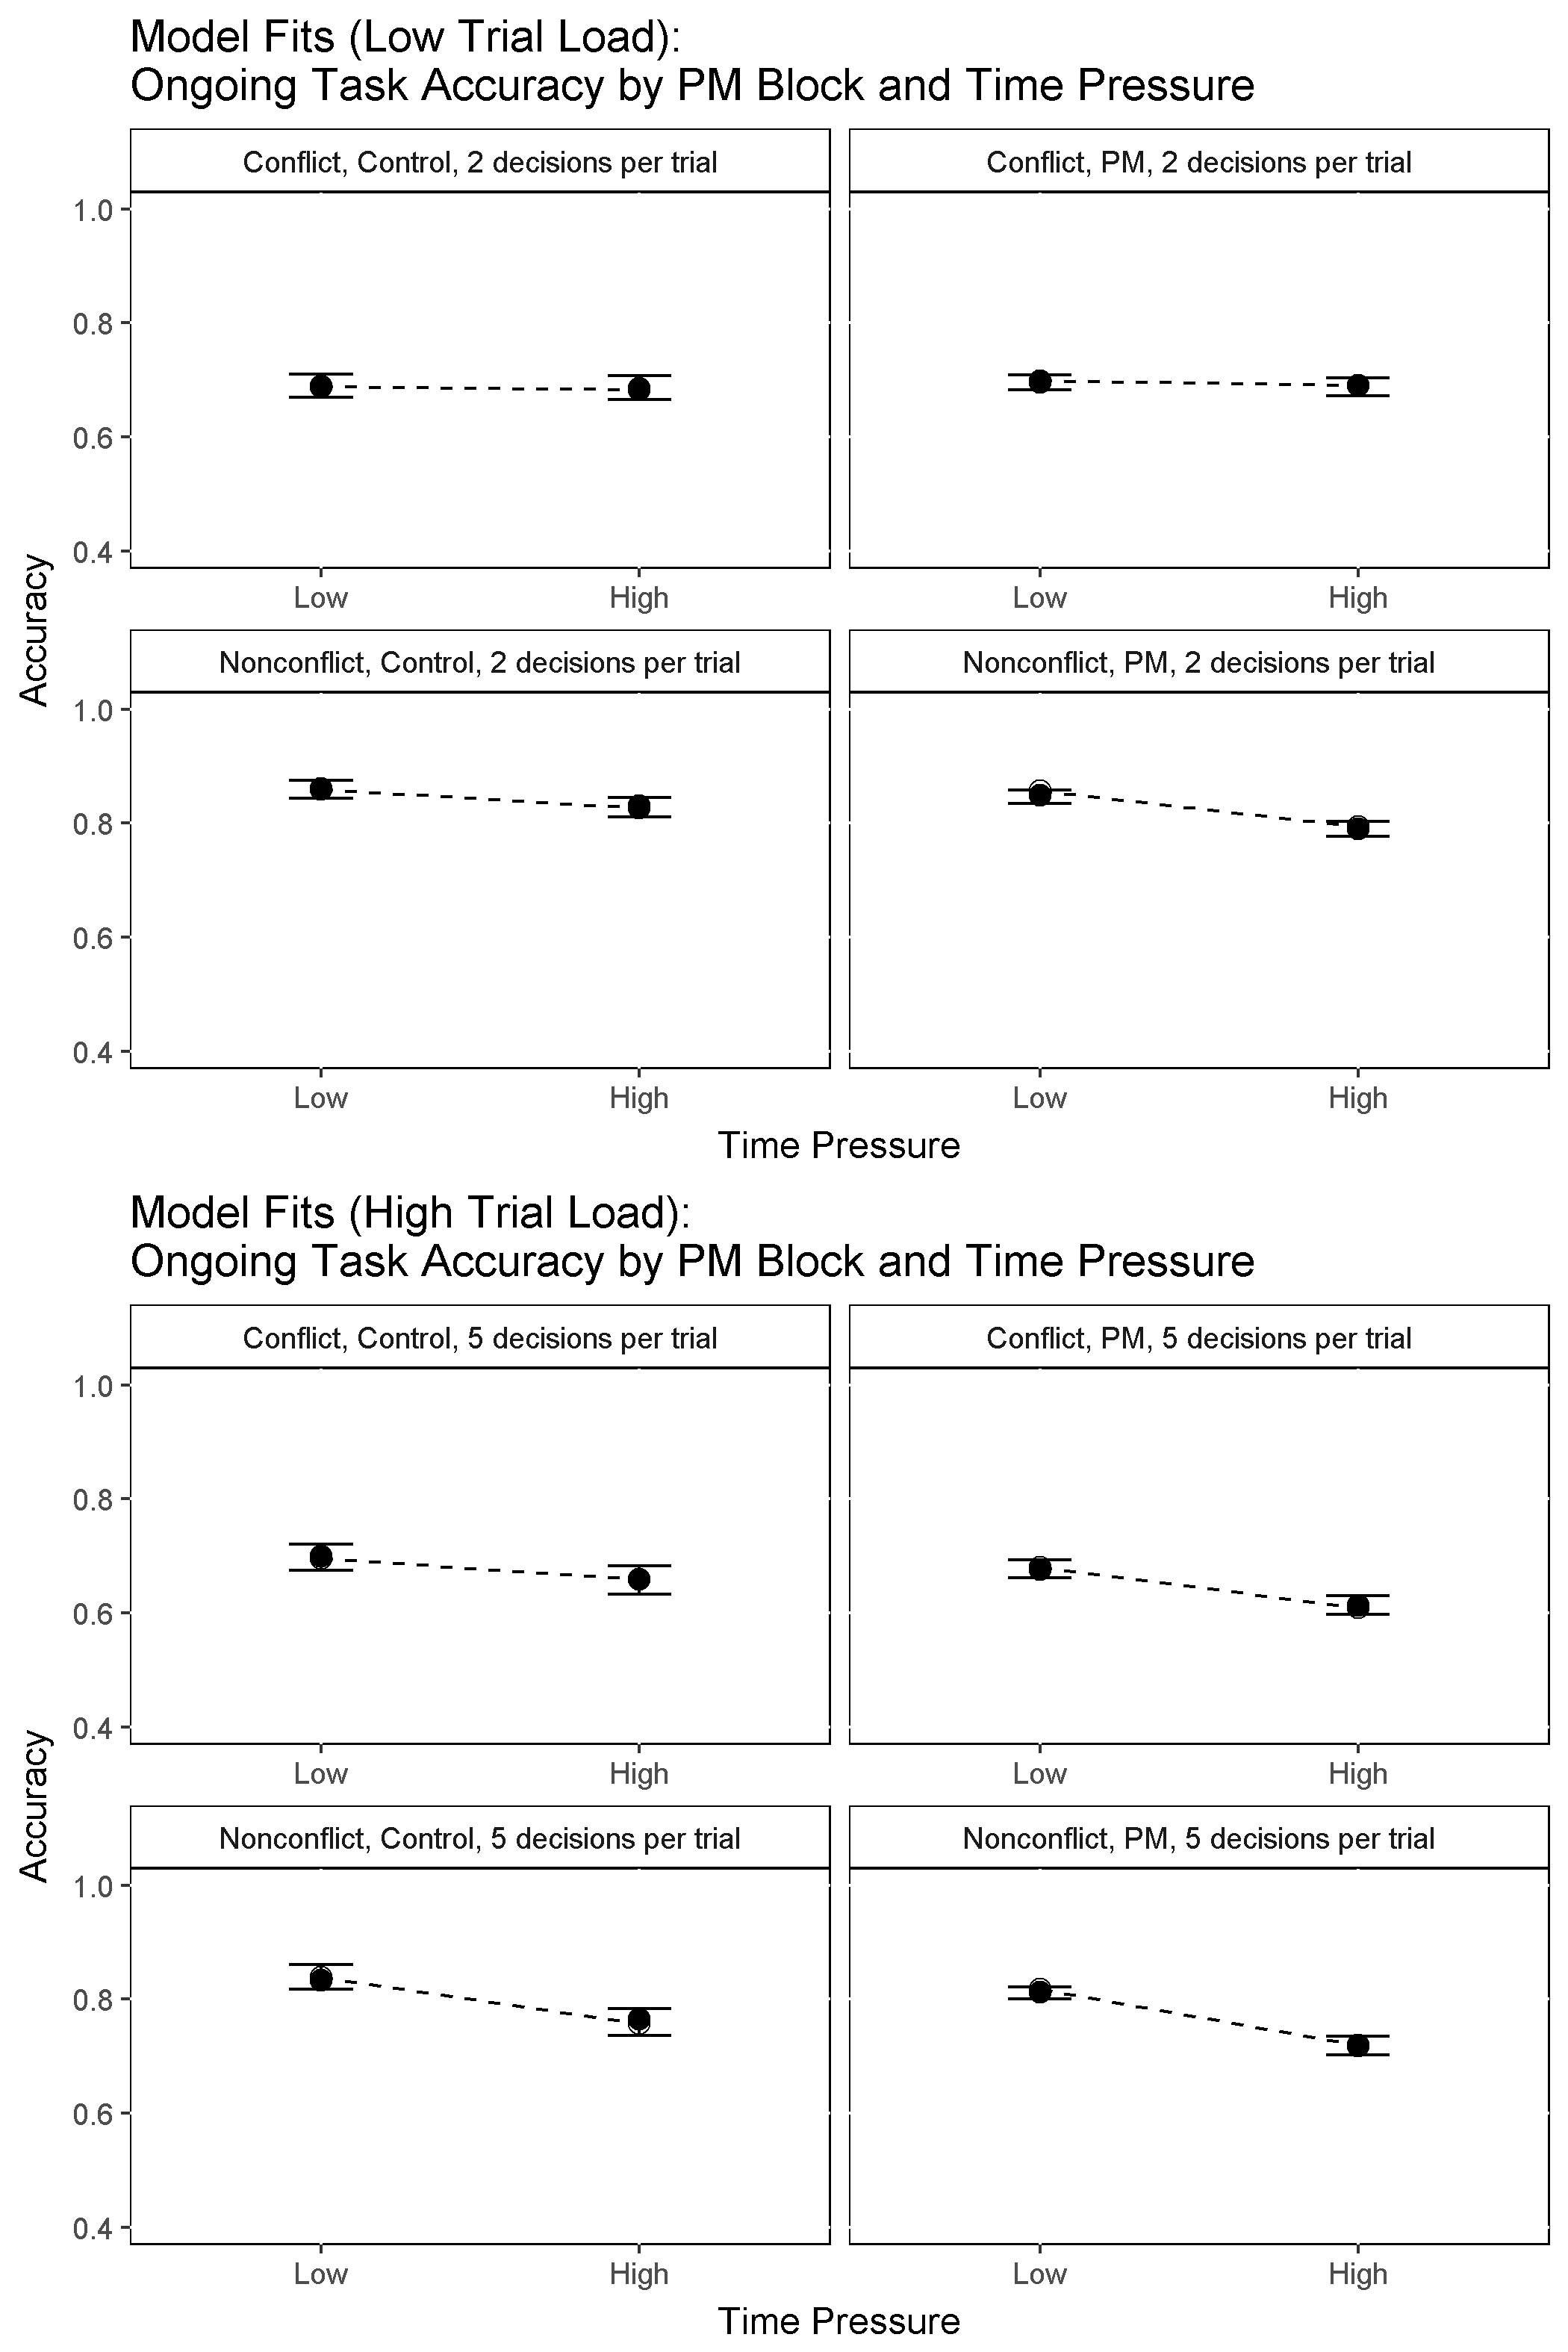
\includegraphics[width=0.8\linewidth]{figures/E1/E1.Fits.Accuracy.Ongoing}
\textbackslash{}caption\{\label{fig:Fits.Accuracy.Ongoing}Model Fits to
Ongoing Task Accuracy. Data effects are represented by white dots. Model
predictions are represented by black dots with 95\% credible
intervals.\}\label{fig:Fit Plot: Accuracy Ongoing}
\textbackslash{}end\{figure\}

\textbackslash{}begin\{figure\}
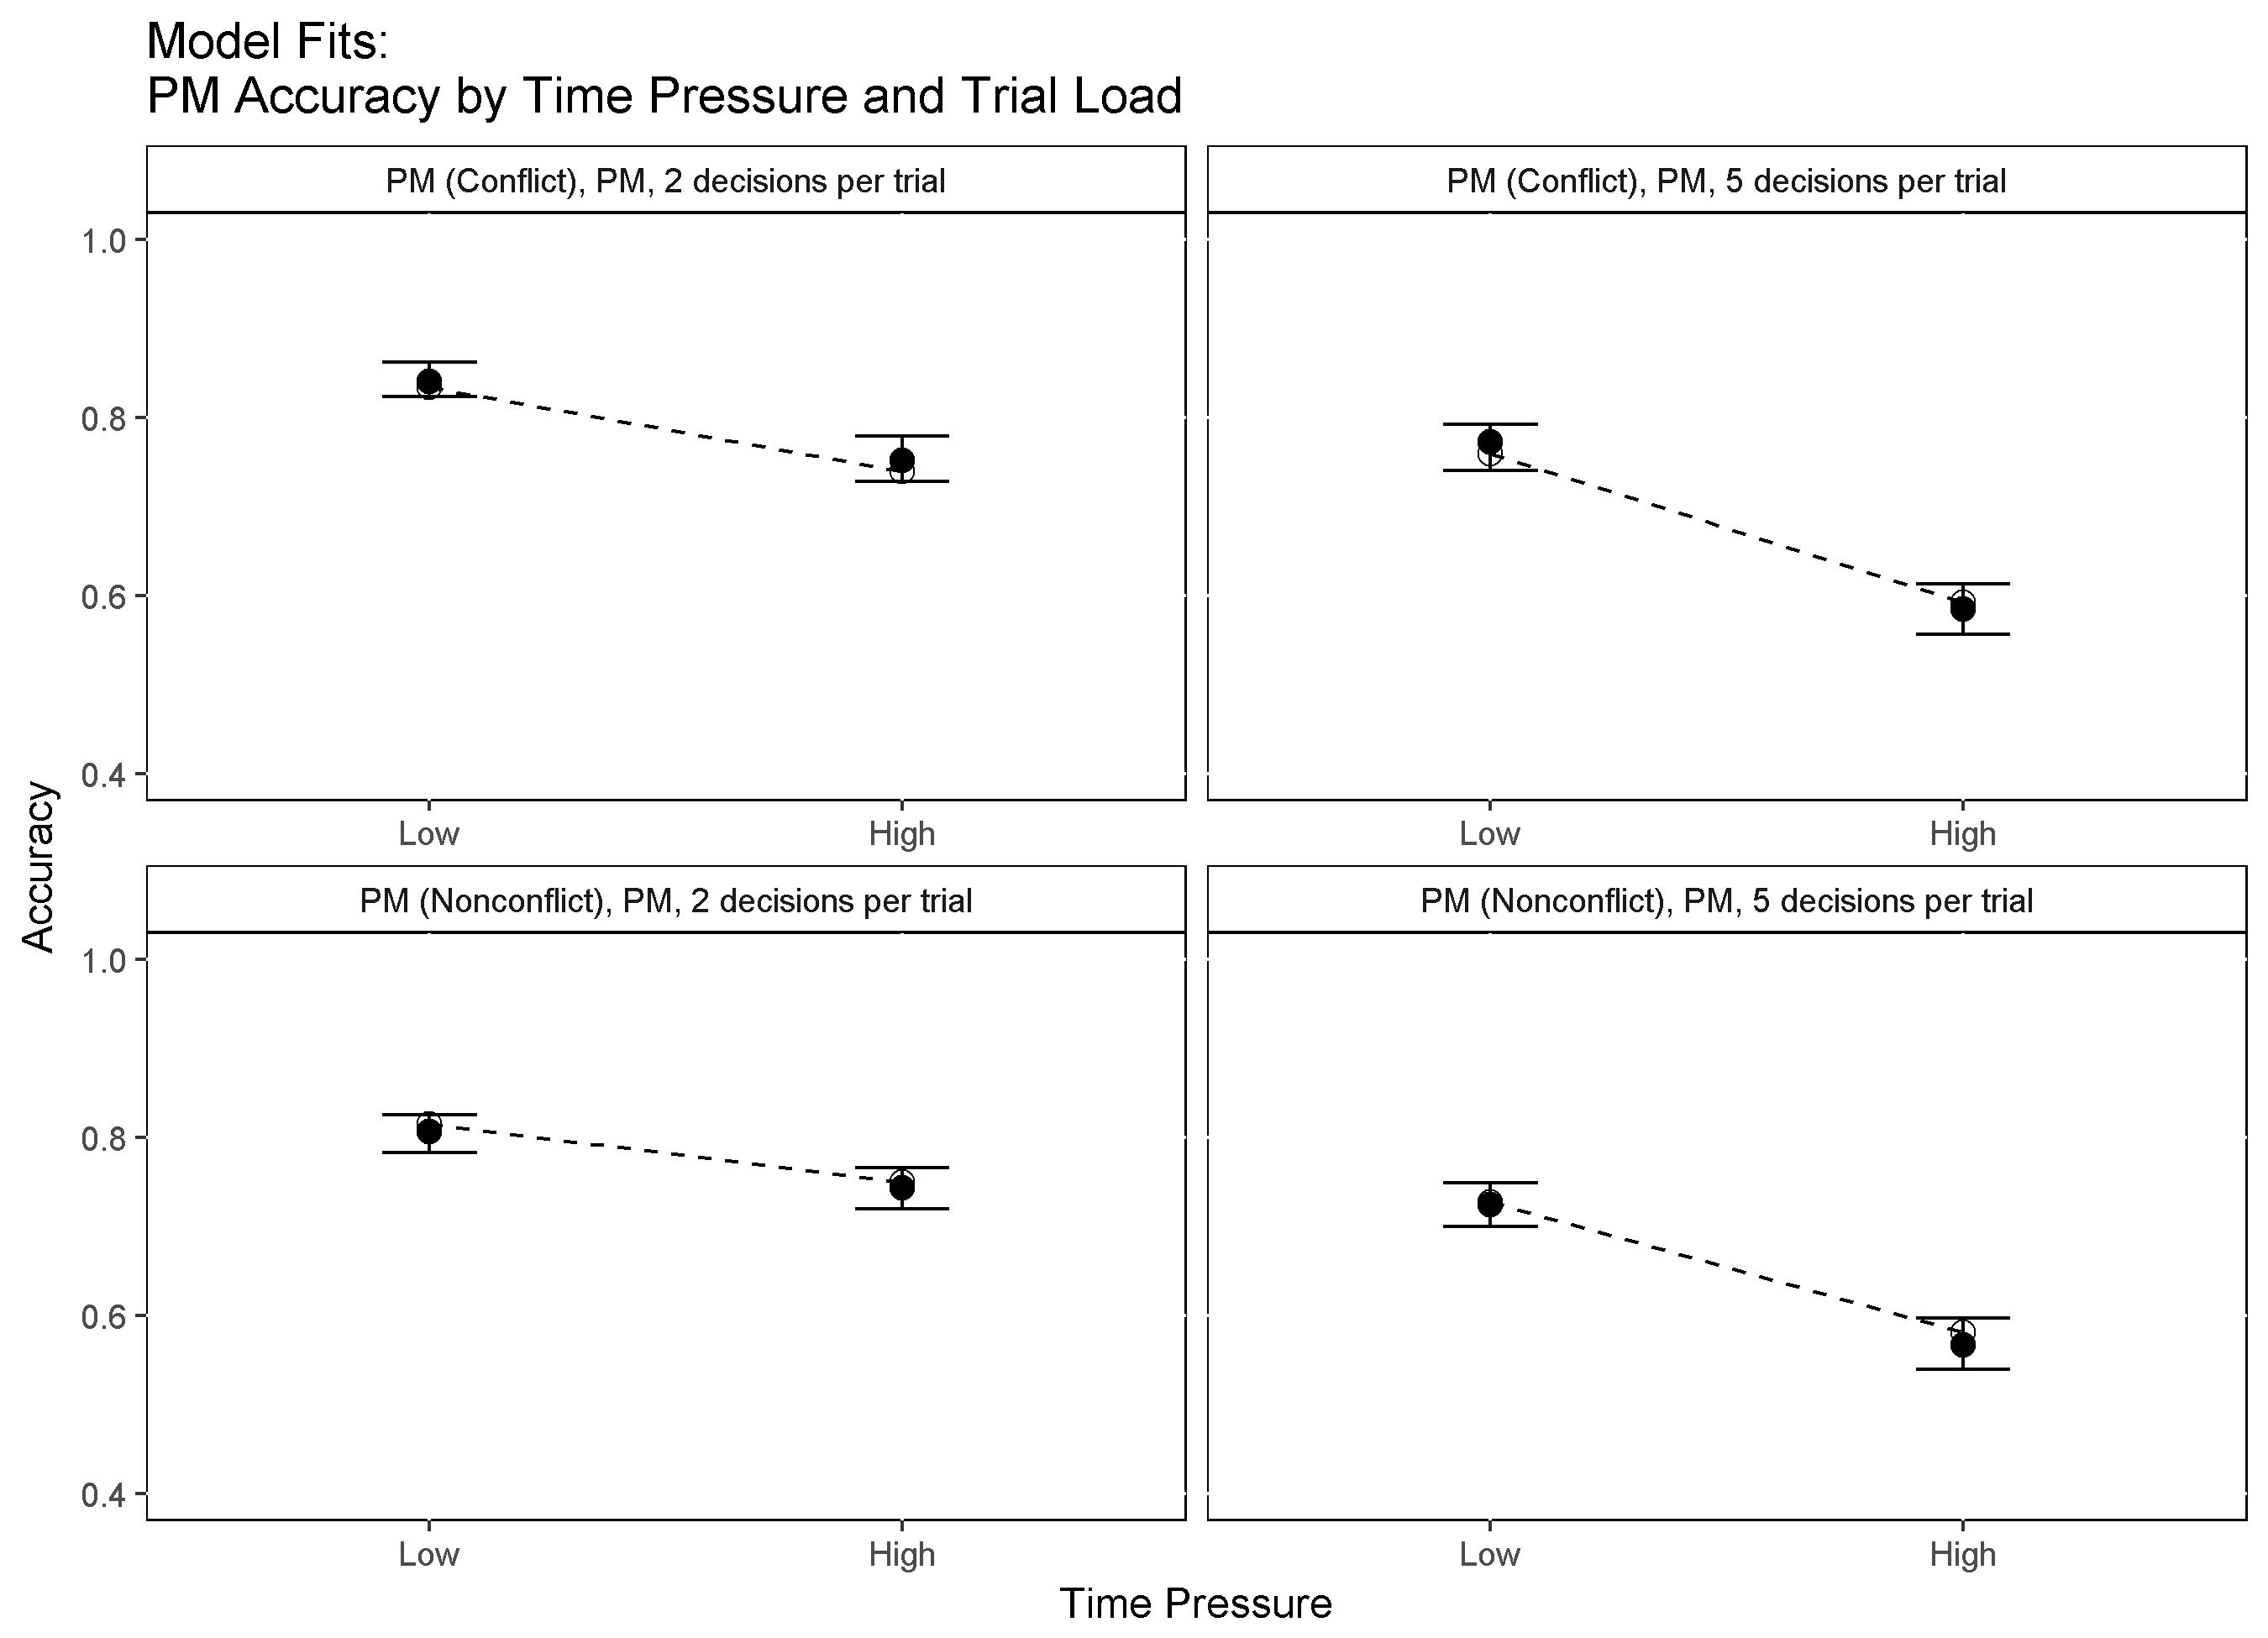
\includegraphics[width=0.8\linewidth]{figures/E1/E1.Fits.Accuracy.PM}
\textbackslash{}caption\{\label{fig:Fits.Accuracy.PM}Model Fits to PM
Accuracy. Data effects are represented by white dots. Model predictions
are represented by black dots with 95\% credible
intervals.\}\label{fig:Fit Plot: Accuracy PM}
\textbackslash{}end\{figure\}

\textbackslash{}begin\{figure\}
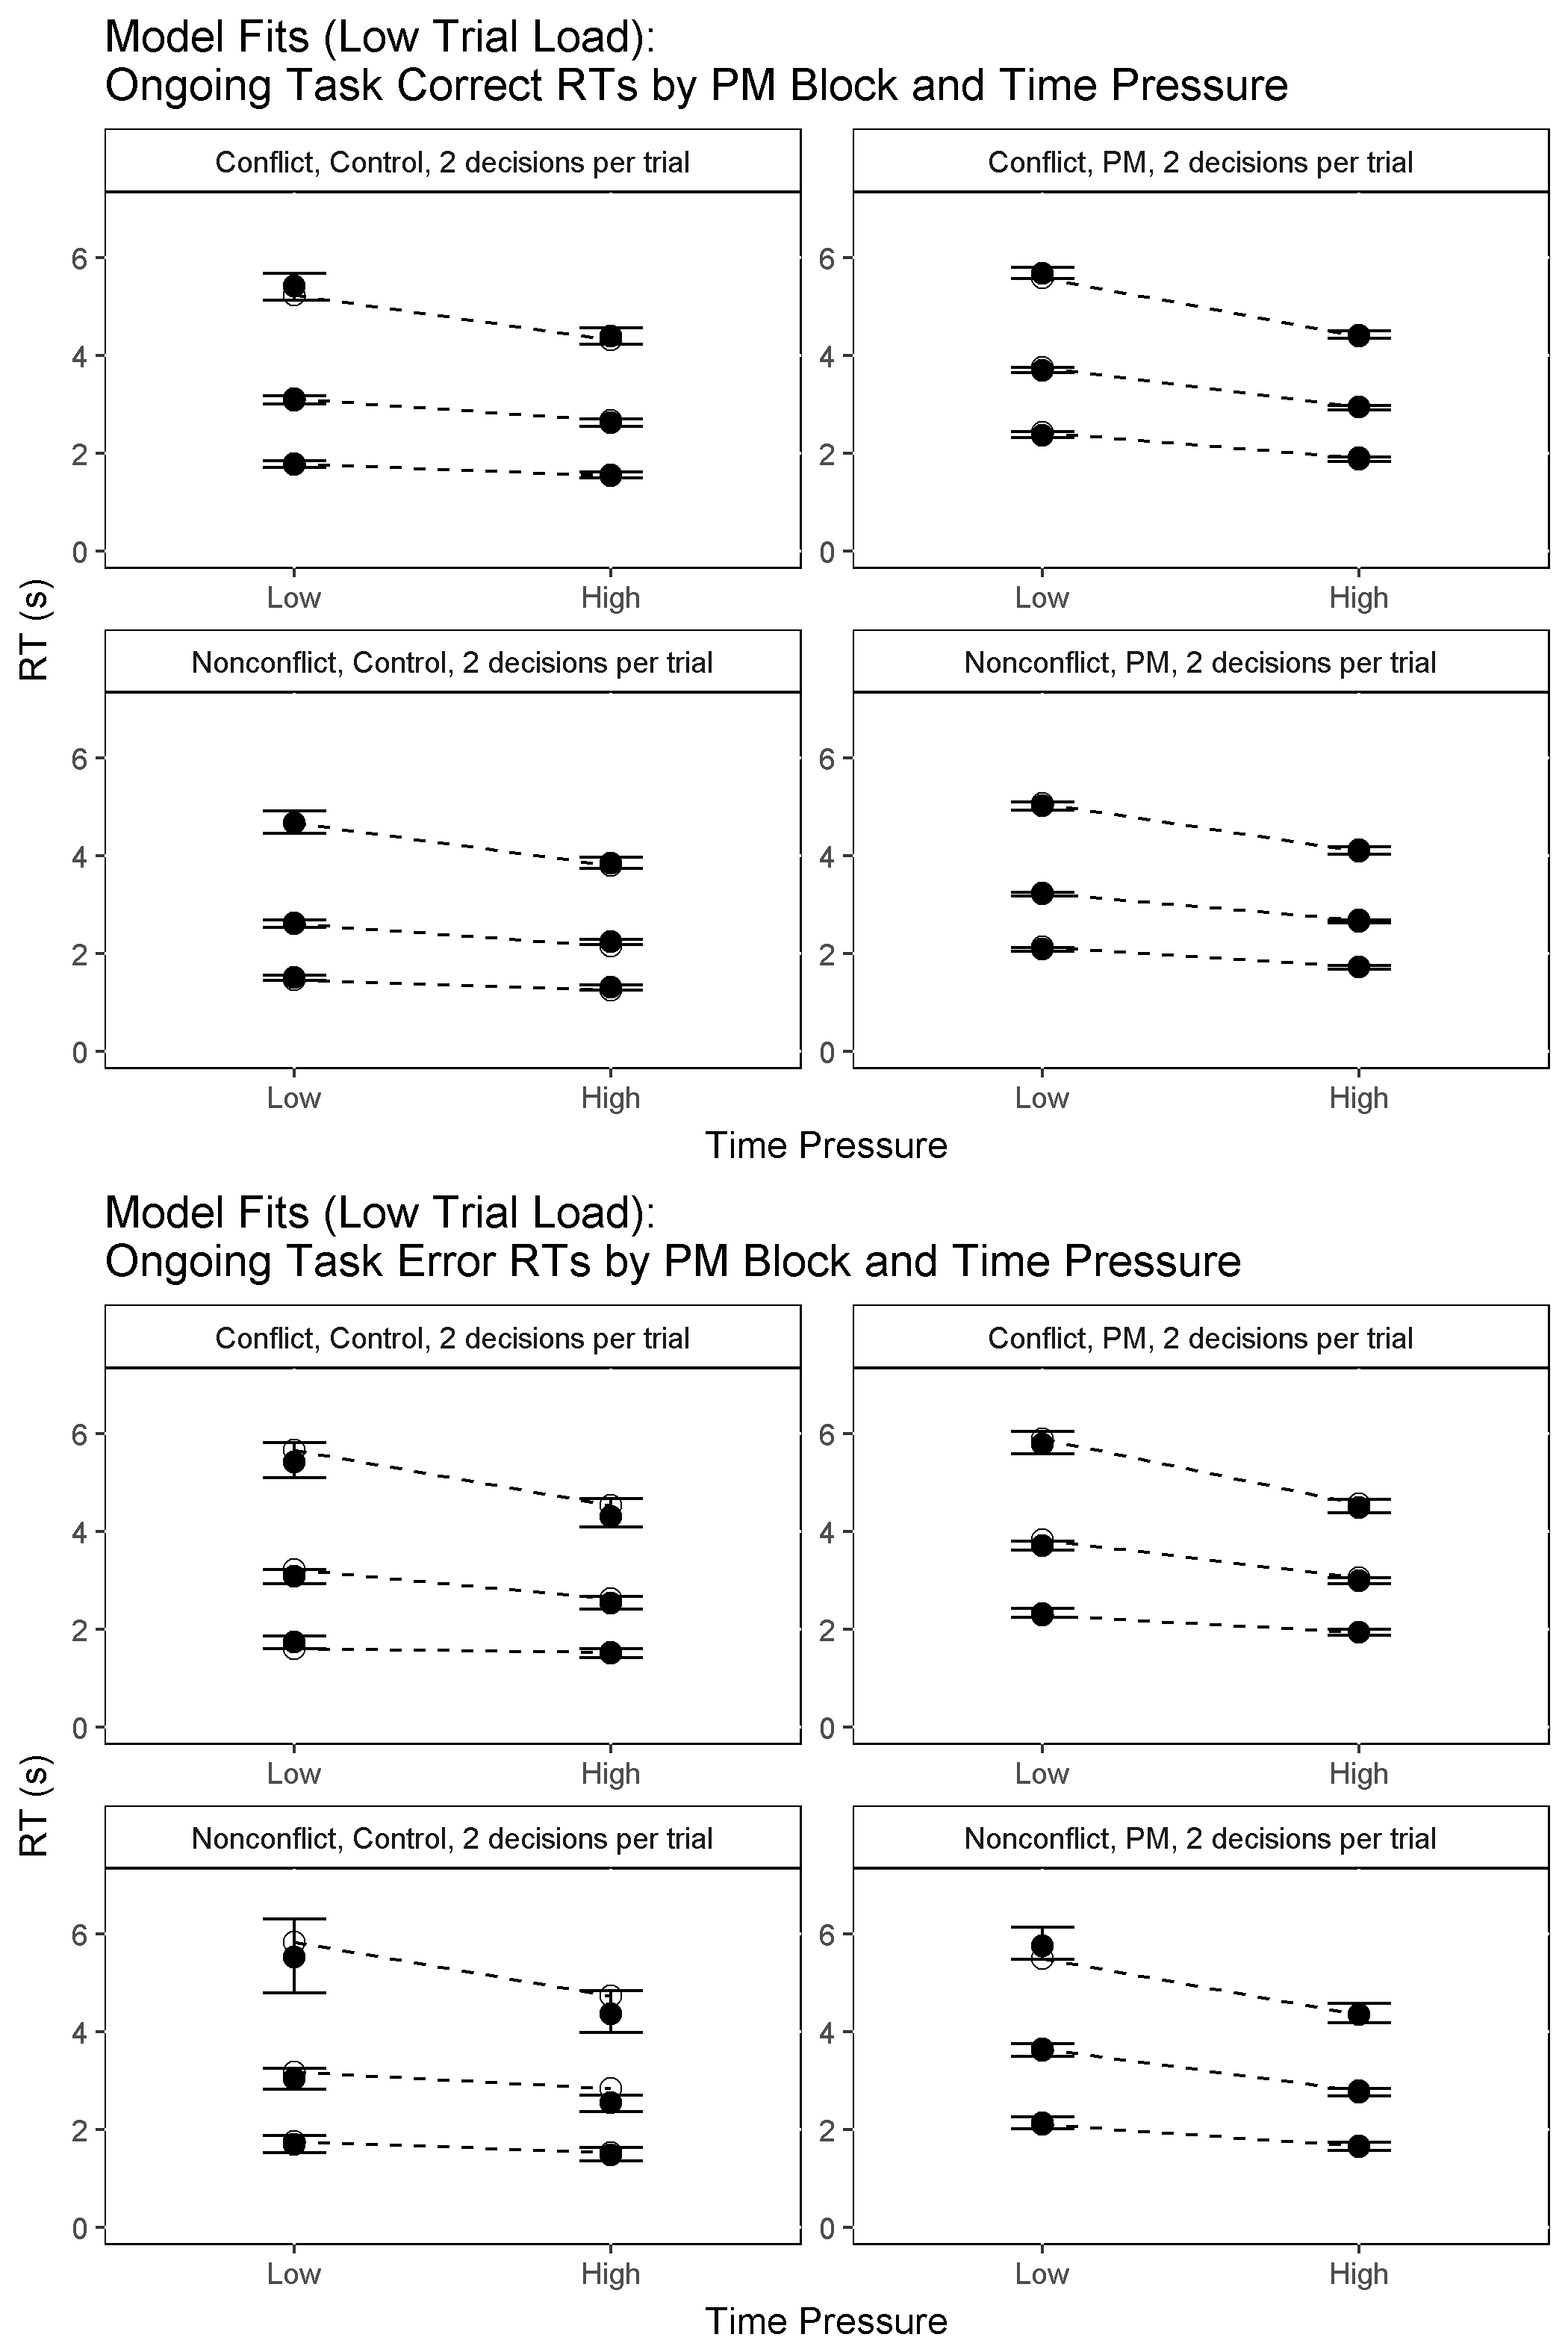
\includegraphics[width=0.8\linewidth]{figures/E1/E1.Fits.RT.Ongoing.2}
\textbackslash{}caption\{\label{fig:Fits.RT.Ongoing.2}Model Fits to
Ongoing Task RT (Low Trial Load). Data effects are represented by white
dots. Model predictions are represented by black dots with 95\% credible
intervals. RT distributions are summarised with three order statistics:
the 0.1 quantile which captures the leading edge of the distribution,
the 0.5 quantile (i.e., the median), and the 0.9 quantile which captures
the tail of the distribution.\}\label{fig:Fit Plot: RT Ongoing Low Load}
\textbackslash{}end\{figure\}

\textbackslash{}begin\{figure\}
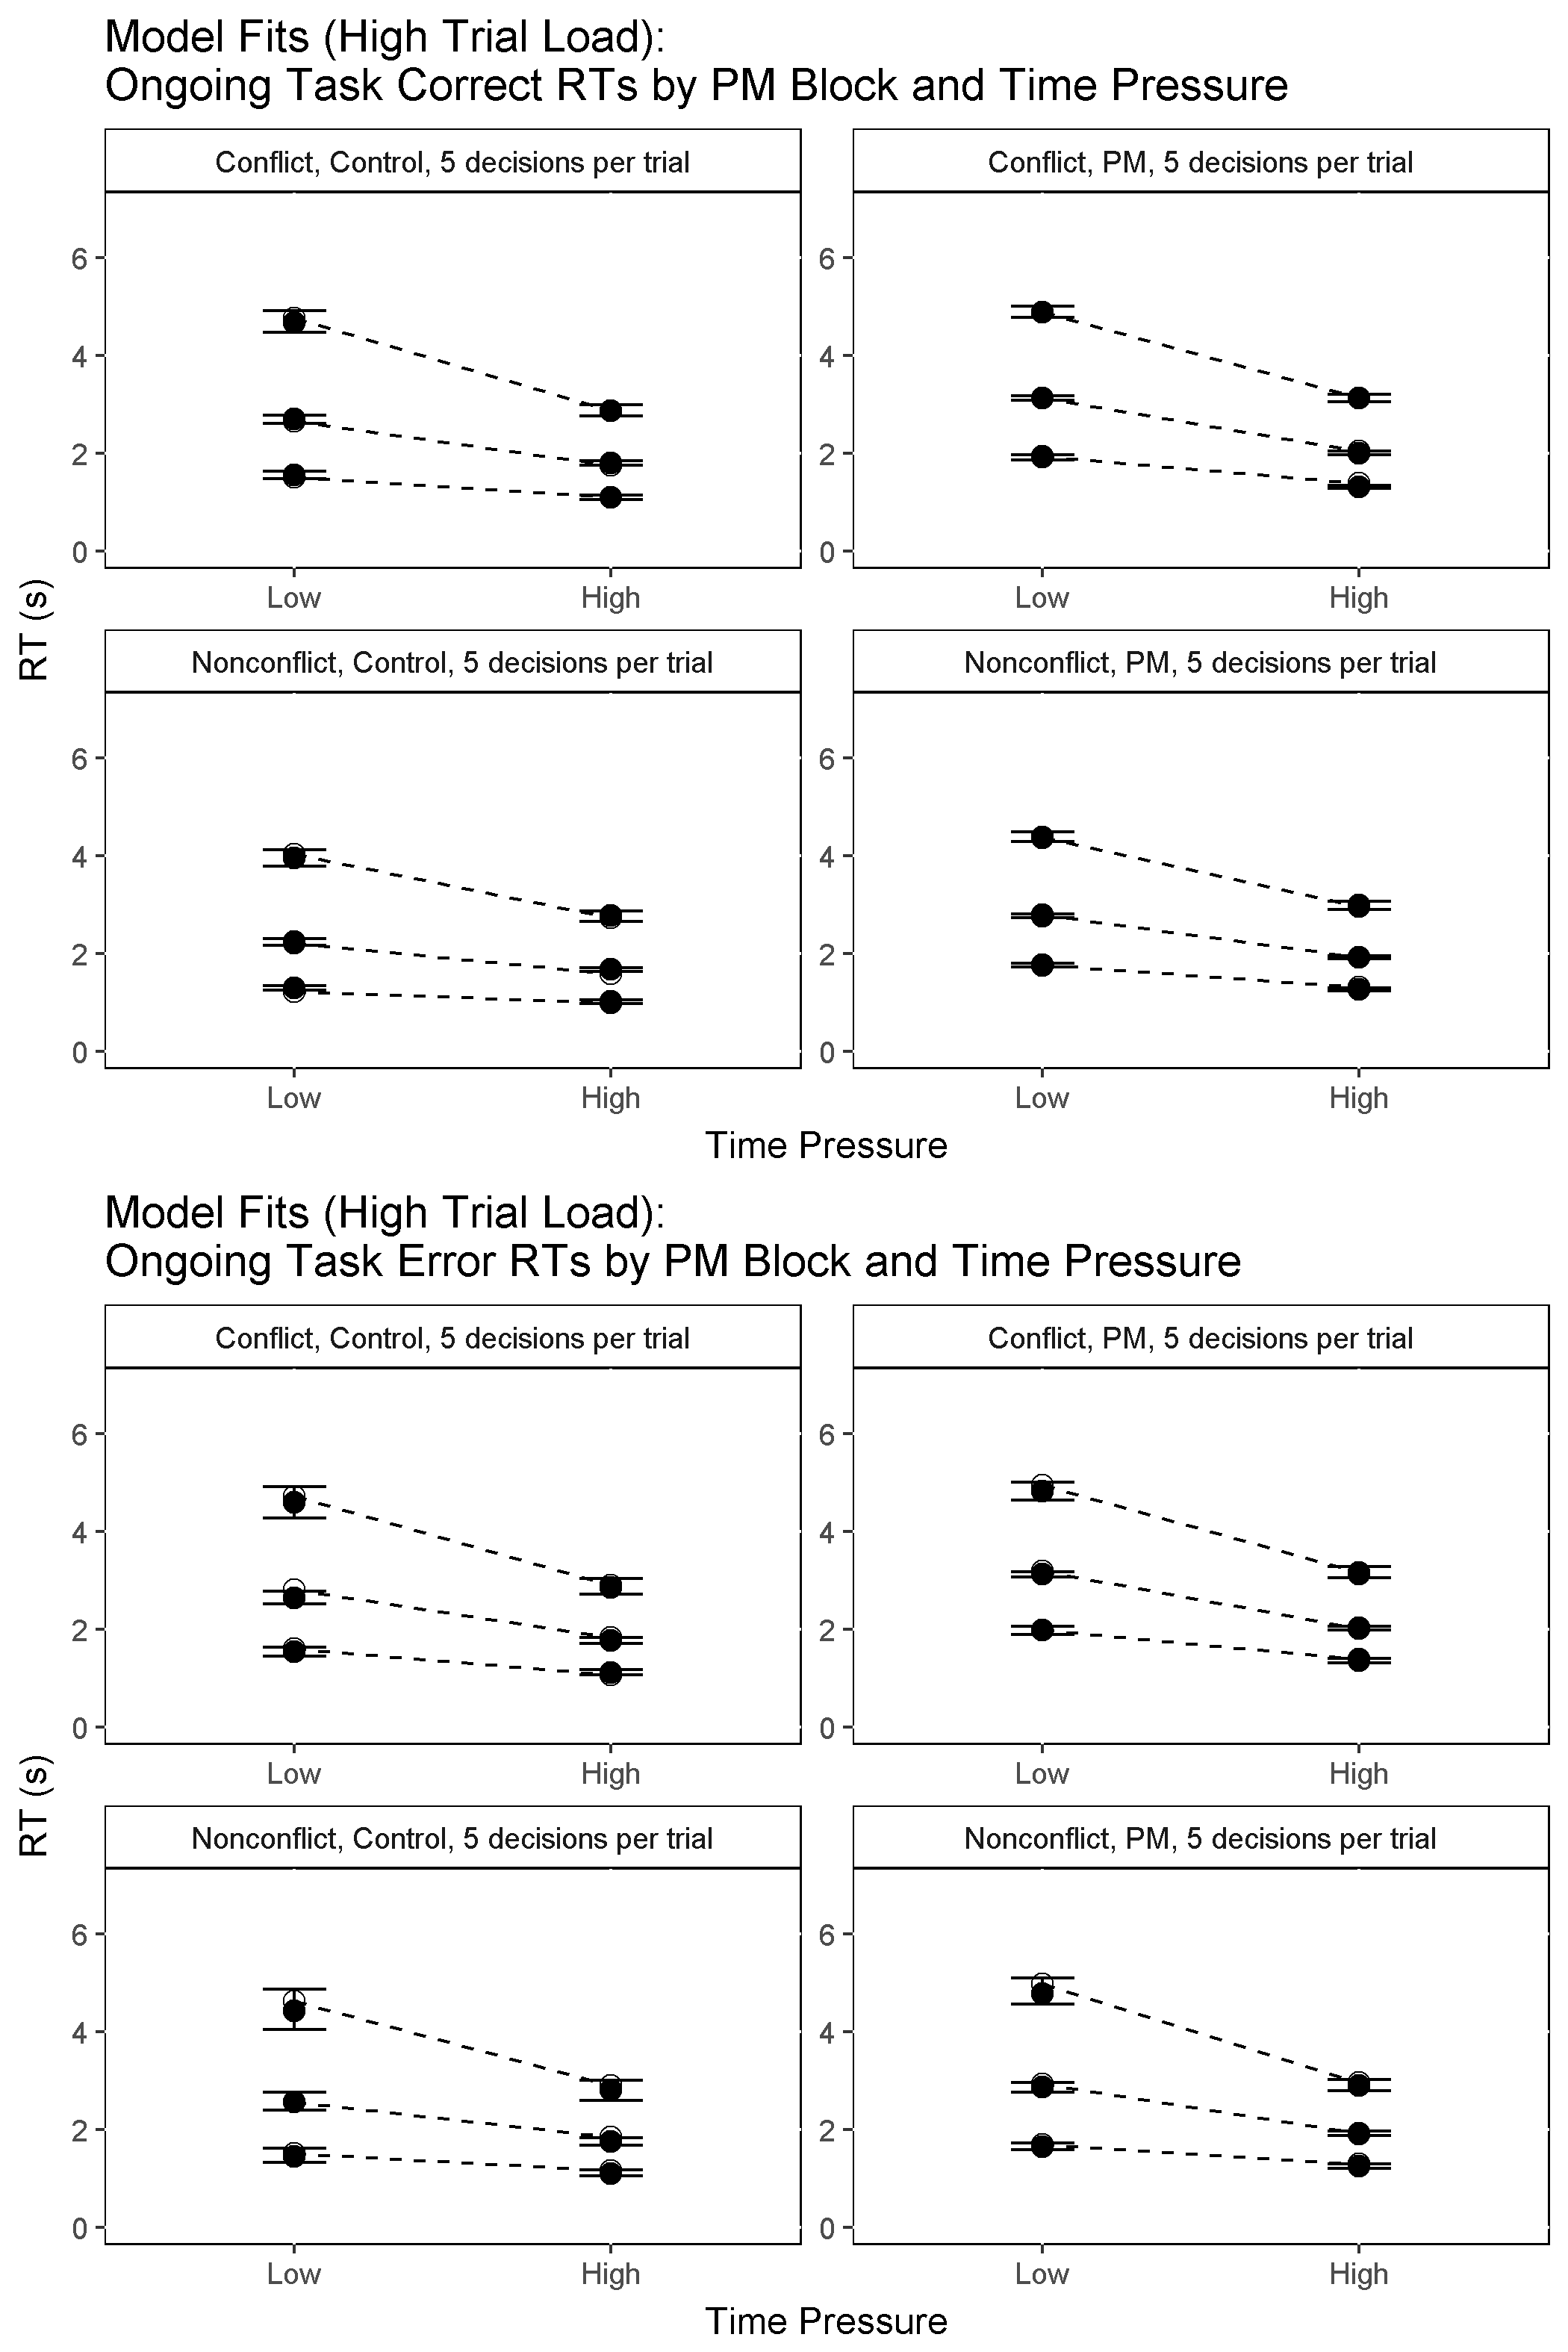
\includegraphics[width=0.8\linewidth]{figures/E1/E1.Fits.RT.Ongoing.5}
\textbackslash{}caption\{\label{fig:Fits.RT.Ongoing.5}Model Fits to
Ongoing Task RT (High Trial Load). Data effects are represented by white
dots. Model predictions are represented by black dots with 95\% credible
intervals. RT distributions are summarised with three order statistics:
the 0.1 quantile which captures the leading edge of the distribution,
the 0.5 quantile (i.e., the median), and the 0.9 quantile which captures
the tail of the
distribution.\}\label{fig:Fit Plot: RT Ongoing High Load}
\textbackslash{}end\{figure\}

\textbackslash{}begin\{figure\}
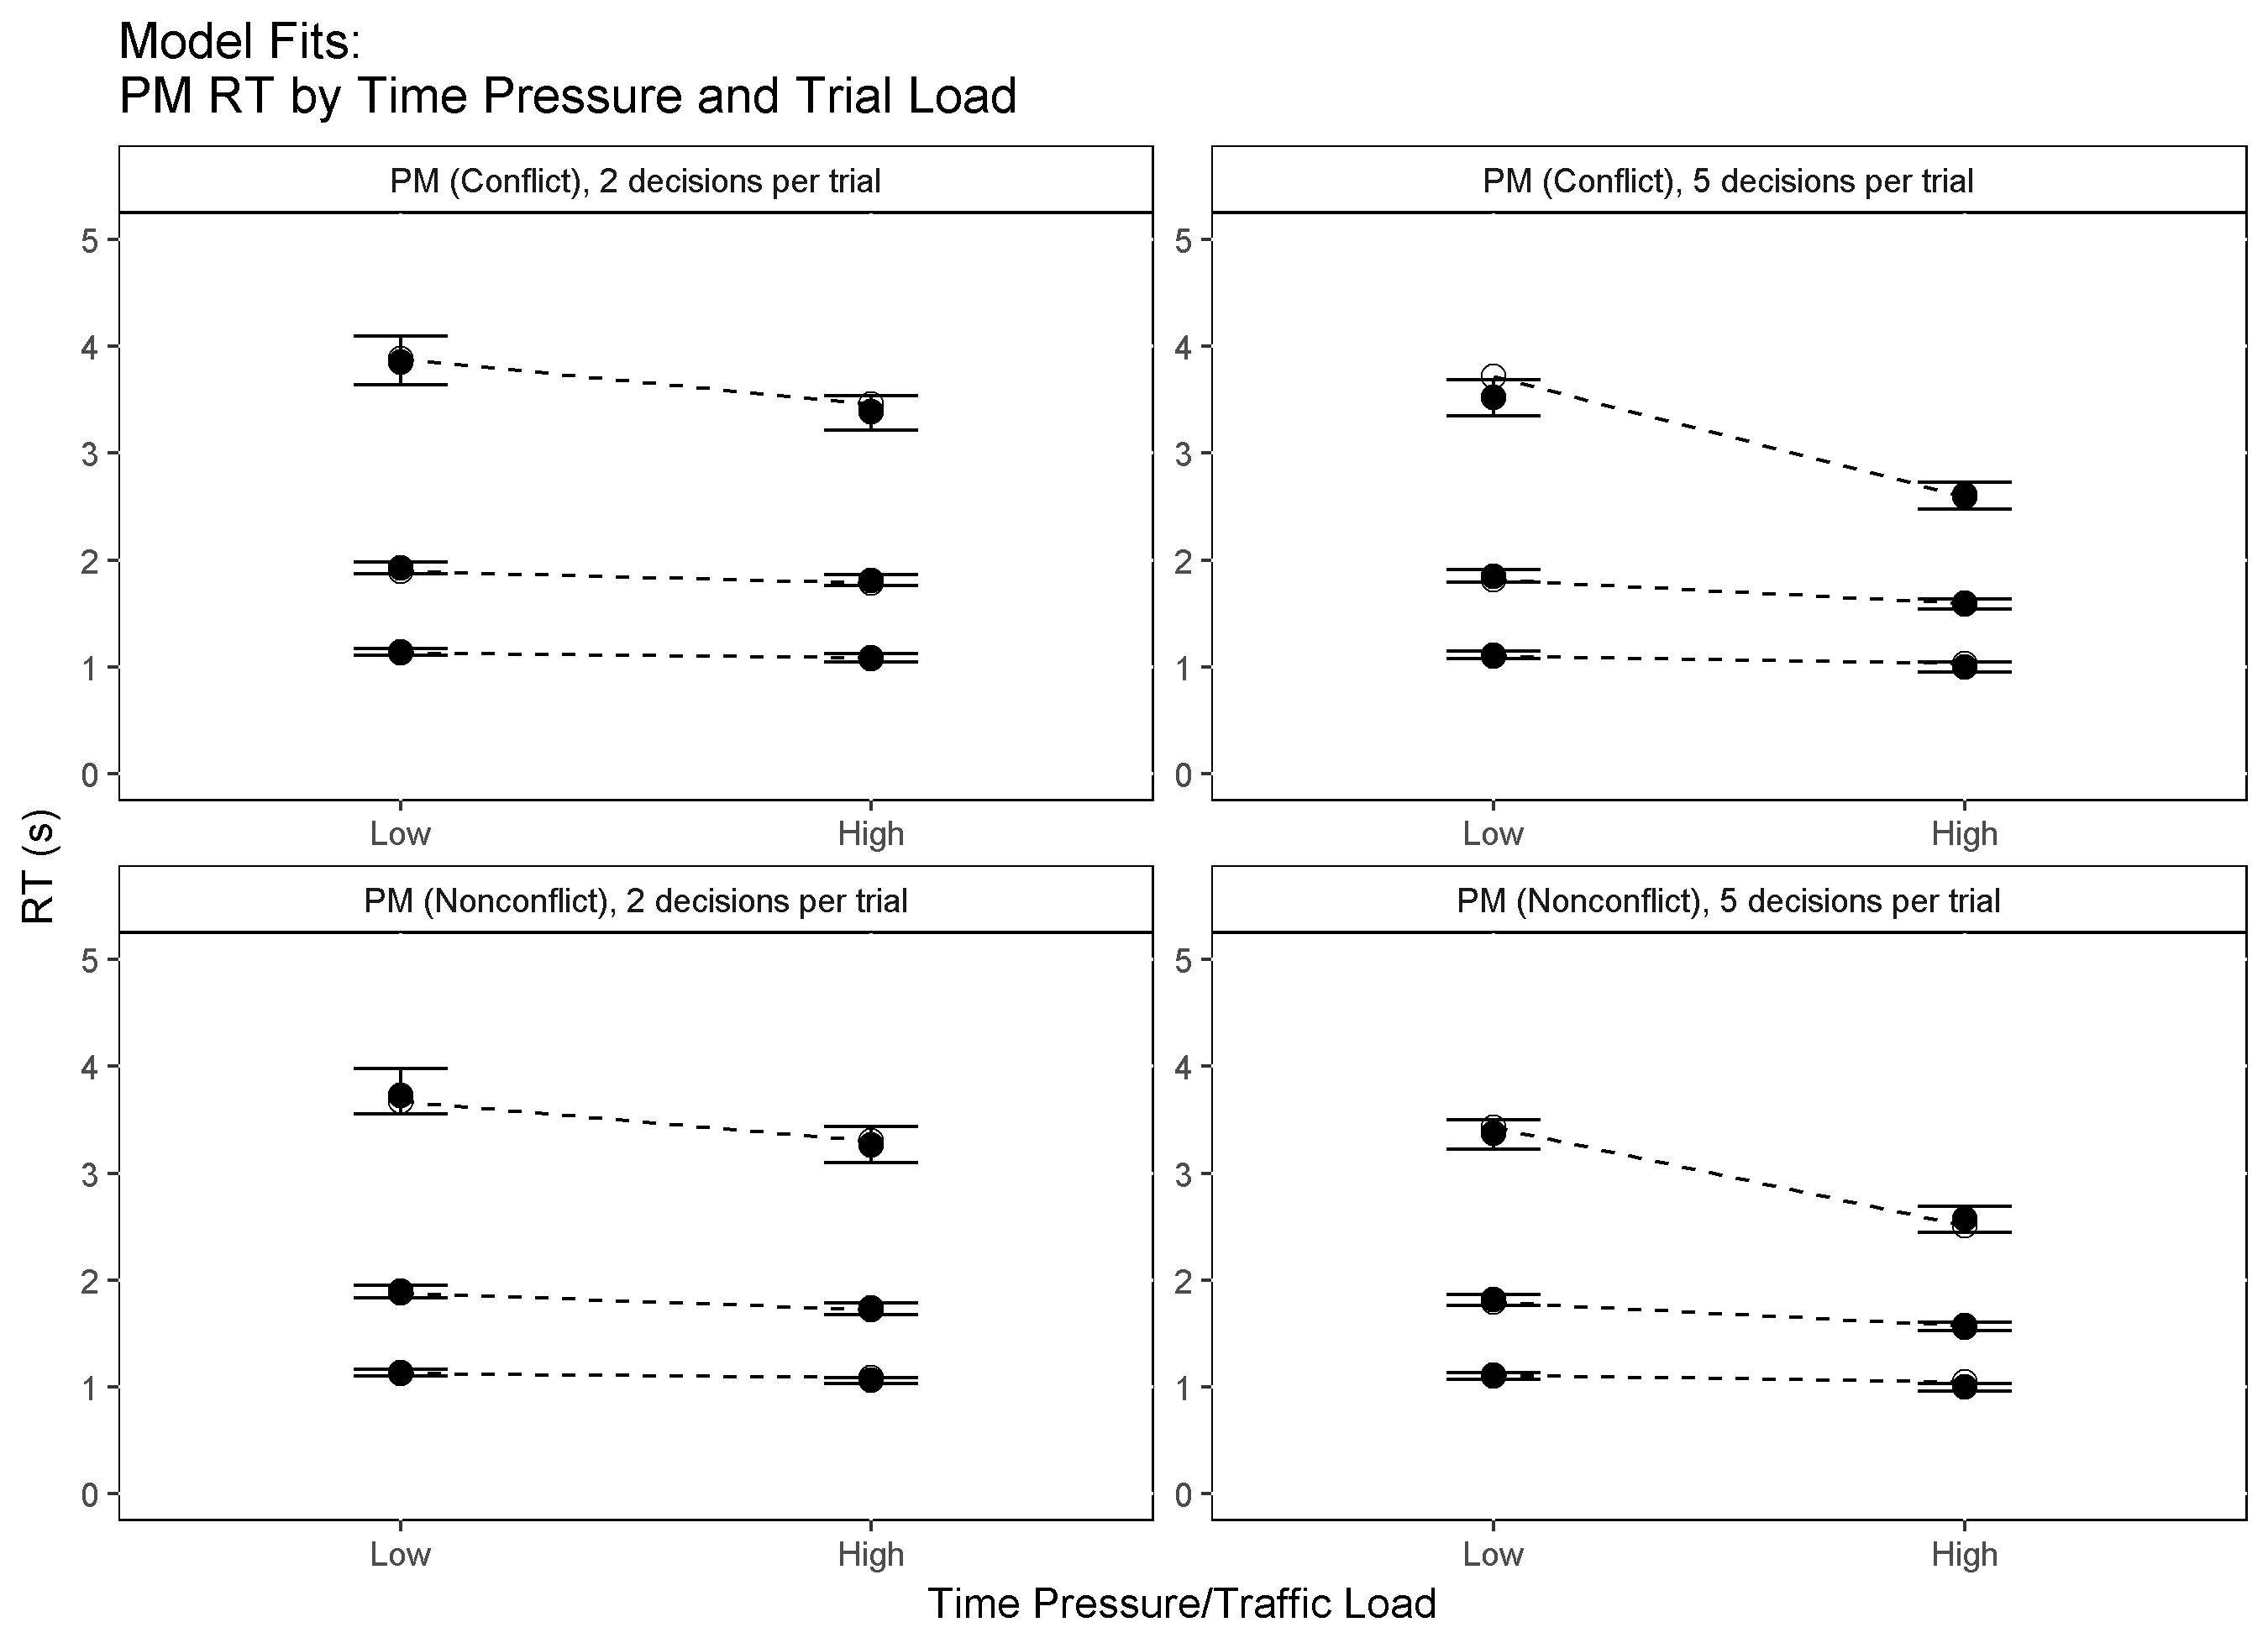
\includegraphics[width=0.8\linewidth]{figures/E1/E1.Fits.RT.PM}
\textbackslash{}caption\{\label{fig:Fits.RT.PM}Model Fits to PM RT. Data
effects are represented by white dots. Model predictions are represented
by black dots with 95\% credible intervals. RT distributions are
summarised with three order statistics: the 0.1 quantile which captures
the leading edge of the distribution, the 0.5 quantile (i.e., the
median), and the 0.9 quantile which captures the tail of the
distribution.\}\label{fig:Fit Plot: RT PM} \textbackslash{}end\{figure\}

\subsubsection{Model Fits: Nonresponse
Proportions}\label{model-fits-nonresponse-proportions}

It should be noted that because the current model was fit to truncated
data (i.e., with nonresponses removed), it is slightly misspecified.
Specifically, because of the response deadline feature in our
experimental design, a small proportion of our data were nonresponses
which do not have associated RTs. As such, they do not contribute
information to RT distributions fit by the LBA model.

Since the model was fit without explicit information about nonresponses,
we were interested in assessing the model's ability to predict
nonresponses and how well those predictions fit empirical nonresponse
proportion data. In order to do this, we simulated data out of the model
and matched the order of the simulated stimuli and responses to the
actual presentation order experienced by each participant. Whenever the
cumulative sum of simulated RTs within a trial exceeded that trial's
deadline, a nonresponse was predicted. Using this method, 100 posterior
predictions for nonresponse proportions were sampled for each
participant and predictions were then averaged over all participants. We
then compared the predicted nonresponses with observed nonresponse
proportions across the different levels of time pressure (i.e.,
different response deadlines) for both low and high trial load
conditions.

Figure \ref{fig:Fits.NR} shows observed versus predicted nonresponse
proportions. As shown, the model's predicted nonresponse proportions
closely match the empirical nonresponse proportions. This gives us
confidence that the slight model misspecification due to fitting to
truncated data is not of concern in terms of the models predictive
validity. To verify this result, we also predicted nonresponses via a
second method in which RT truncation was built-in to the simulation
rather than RTs being censored after simulation. The fits produced by
this method were not noticeably different than the fits presented.

\textbackslash{}begin\{figure\}
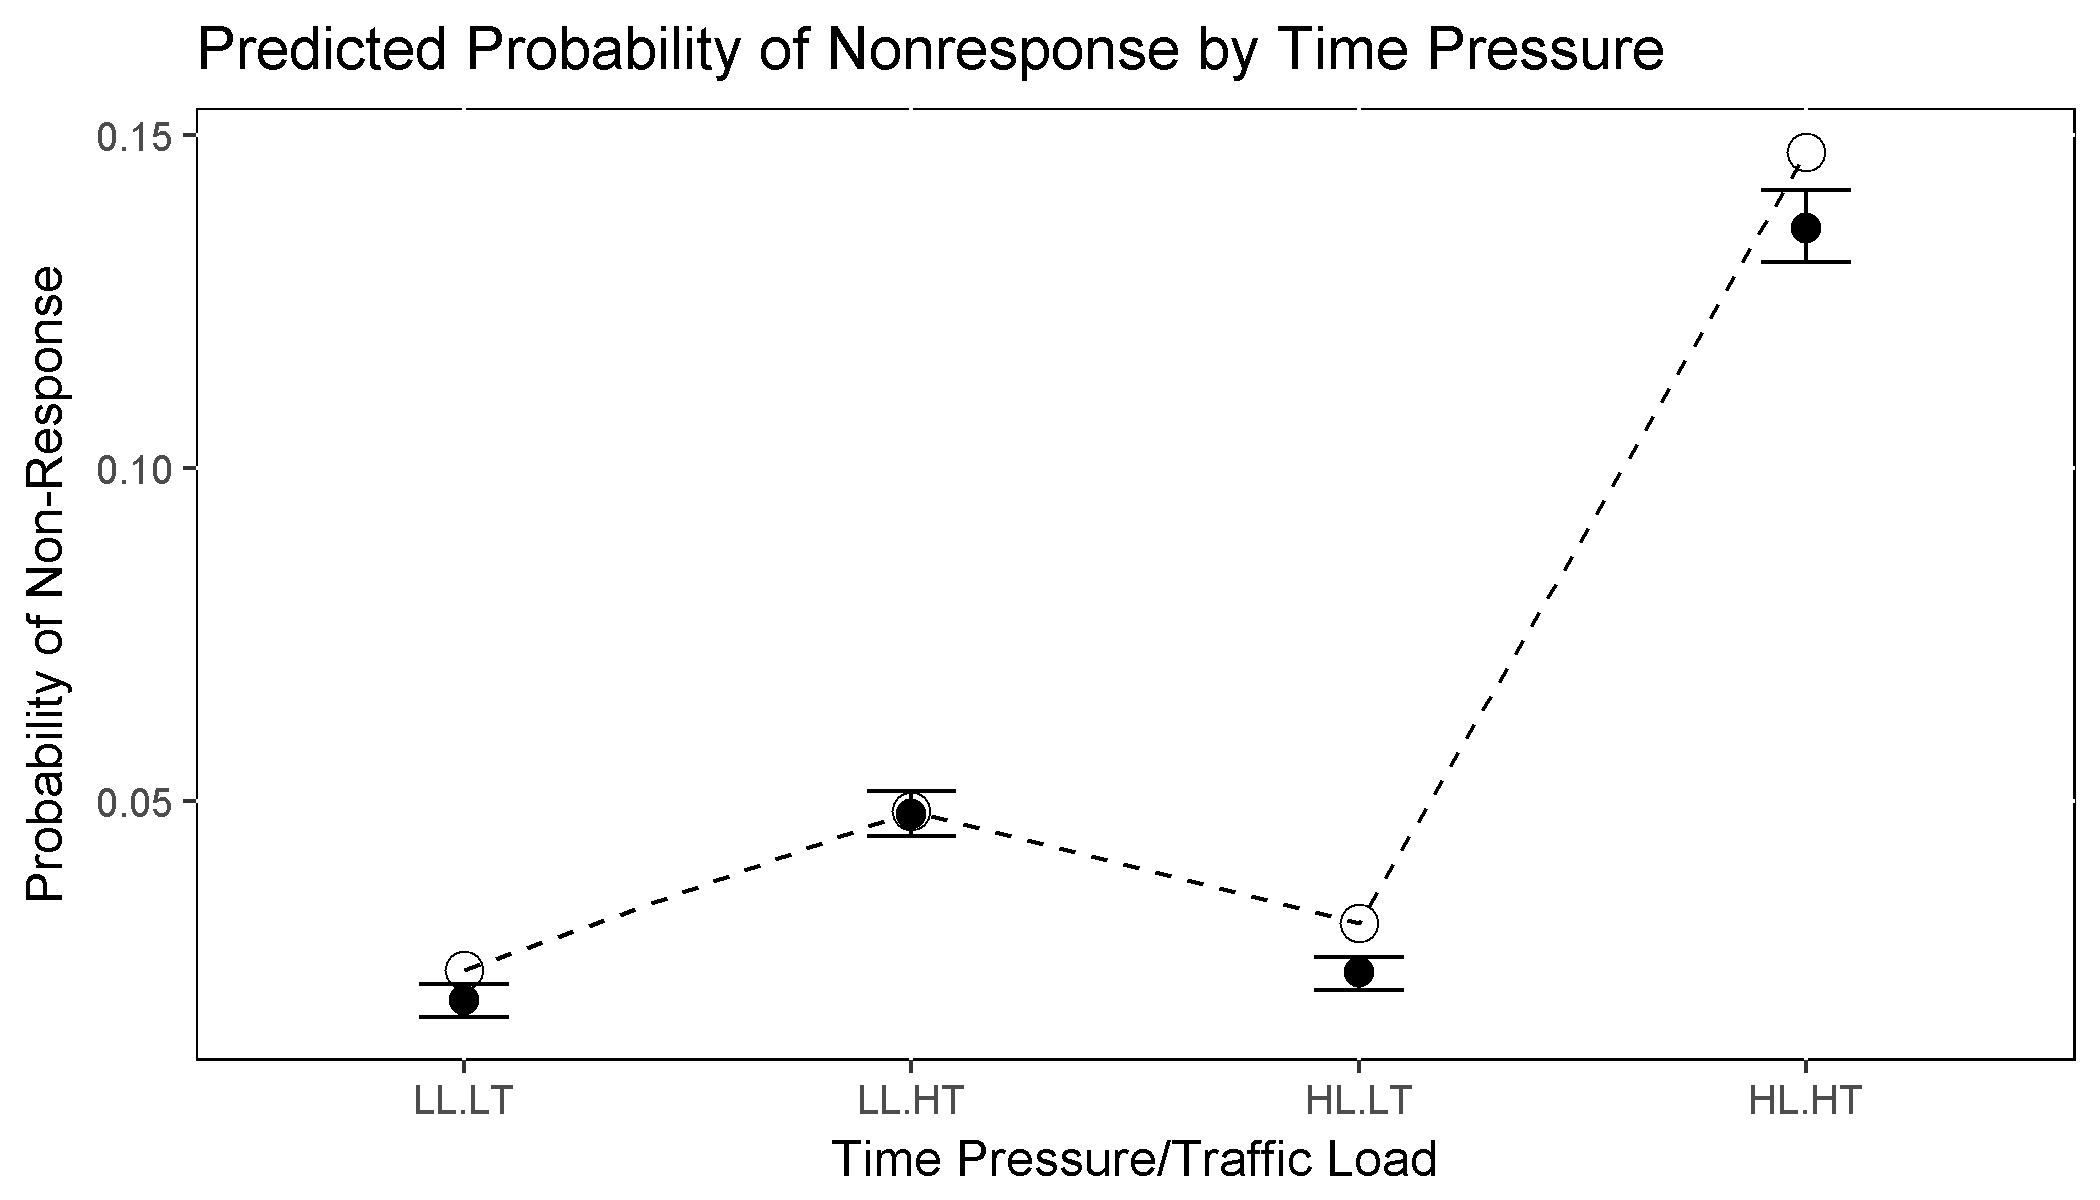
\includegraphics[width=0.8\linewidth]{figures/E1/E1.Fits.NR}
\textbackslash{}caption\{\label{fig:Fits.NR}Model Fits to Nonresponse
Proportions. Data effects are represented by white dots. Model
predictions are represented by black dots with 95\% credible
intervals.\}\label{fig:Fit Plot: Nonresponses}
\textbackslash{}end\{figure\}

\subsubsection{Model Selection}\label{model-selection}

We applied model selection to assess whether we could justify
contstraining model parameters over blocked experimental conditions
(e.g., Control/PM Block, Time Pressure) to obtain a simpler model with
fewer parameters. To select between models, we used the Deviance
Information Criterion (DIC), a measure which takes into account both
goodness of fit and model complexity (number of parameters). In general,
models with smaller DIC values are to be prefered as more parsimonious
explanations of the data than models with larger DIC values. Table XX
shows each model we compared, its number of parameters, and its
corresponding DIC value.

\begin{longtable}[]{@{}lcc@{}}
\caption{DIC Model Selection. Lower DIC indicates more preference for
the model.}\tabularnewline
\toprule
\begin{minipage}[b]{0.35\columnwidth}\raggedright\strut
Model\strut
\end{minipage} & \begin{minipage}[b]{0.19\columnwidth}\centering\strut
N Parameters\strut
\end{minipage} & \begin{minipage}[b]{0.08\columnwidth}\centering\strut
DIC\strut
\end{minipage}\tabularnewline
\midrule
\endfirsthead
\toprule
\begin{minipage}[b]{0.35\columnwidth}\raggedright\strut
Model\strut
\end{minipage} & \begin{minipage}[b]{0.19\columnwidth}\centering\strut
N Parameters\strut
\end{minipage} & \begin{minipage}[b]{0.08\columnwidth}\centering\strut
DIC\strut
\end{minipage}\tabularnewline
\midrule
\endhead
\begin{minipage}[t]{0.35\columnwidth}\raggedright\strut
Top Model\strut
\end{minipage} & \begin{minipage}[t]{0.19\columnwidth}\centering\strut
89\strut
\end{minipage} & \begin{minipage}[t]{0.08\columnwidth}\centering\strut
187068\strut
\end{minipage}\tabularnewline
\begin{minipage}[t]{0.35\columnwidth}\raggedright\strut
Selected Model\strut
\end{minipage} & \begin{minipage}[t]{0.19\columnwidth}\centering\strut
84\strut
\end{minipage} & \begin{minipage}[t]{0.08\columnwidth}\centering\strut
186995\strut
\end{minipage}\tabularnewline
\begin{minipage}[t]{0.35\columnwidth}\raggedright\strut
Selected Model with B fixed over PM Block\strut
\end{minipage} & \begin{minipage}[t]{0.19\columnwidth}\centering\strut
81\strut
\end{minipage} & \begin{minipage}[t]{0.08\columnwidth}\centering\strut
190690\strut
\end{minipage}\tabularnewline
\begin{minipage}[t]{0.35\columnwidth}\raggedright\strut
Selected Model with V fixed over PM Block\strut
\end{minipage} & \begin{minipage}[t]{0.19\columnwidth}\centering\strut
73\strut
\end{minipage} & \begin{minipage}[t]{0.08\columnwidth}\centering\strut
188370\strut
\end{minipage}\tabularnewline
\begin{minipage}[t]{0.35\columnwidth}\raggedright\strut
Selected Model with B fixed over Time Pressure\strut
\end{minipage} & \begin{minipage}[t]{0.19\columnwidth}\centering\strut
74\strut
\end{minipage} & \begin{minipage}[t]{0.08\columnwidth}\centering\strut
190640\strut
\end{minipage}\tabularnewline
\begin{minipage}[t]{0.35\columnwidth}\raggedright\strut
Selected Model with V fixed over Time Pressure\strut
\end{minipage} & \begin{minipage}[t]{0.19\columnwidth}\centering\strut
47\strut
\end{minipage} & \begin{minipage}[t]{0.08\columnwidth}\centering\strut
190742\strut
\end{minipage}\tabularnewline
\bottomrule
\end{longtable}

Starting with the fully flexible top model, we built several simpler
variants by systematically constraining threshold and rate parameters
over PM and time pressure factors. This allowed us to assess whether it
was necessary to vary thresholds and/or rates to account for observed PM
demand and time pressure effects. We compared the following four
constrained models to the top model: a model in which rates could vary
across PM and control blocks but thresholds could not; a model in which
thresholds could vary across PM and control blocks but rates could not;
a model in which rates could vary by time pressure but thresholds could
not; and a model in which thresholds could vary by time pressure but
rates could not.

As Table XX shows, in each case the simpler model was rejected in favour
of the fully flexible top model, suggesting that it is necessary to
allow both rate and threshold parameters to vary over PM and time
pressure (i.e., both parameters are influenced by PM and time pressure
manipulations and are important in explaining the observed data).

Finally, we tested an additional model (the selected model) which
allowed both rates and thresholds to vary over both PM and time
pressure, but included a slight simplification from the top model. The
simplification involved constraining the PM rate parameter such that it
was not allowed to vary over stimulus type (i.e., PM conflicts and PM
nonconflicts had the same accumulation rate). This simplification makes
theoretical sense, since the evidence used to make a PM decision (i.e.,
particular letters in an aircraft callsign) is independent of the
evidence used to make either conflict or nonconflict ongoing task
decisions (i.e., speed, relative distance, and motion). This slightly
simpler model produced the smallest DIC value and was thus selected as
our preferred model.

Although the results of model selection suggest that both rates and
thresholds have some role in explaining PM cost and time pressure
effects, we cannot say how important each parameter is or what
proportion of a given effect is accounted for by each parameter. As
such, in the next section we test the direction and magnitude of
differences between conditions in the parameters of the selected model.
Testing the direction of effects is important because it allows us to
distinguish between competing theories of PM costs, whose predictions
are also directional (e.g., capacity-sharing theories predict lower
accumulation rates under PM load than control). Testing the magnitude of
effects is similarly important, especially in applied settings, as it
indicates which processes contribute the most to a given effect (such as
PM costs) or are most affected by an experimental manipulation.

\subsection{Model Summary}\label{model-summary}

To summarise the central tendency of model parameters over participants,
we created a subject-average posterior distribution. This was obtained
by computing the mean of each posterior sample over all participants for
each parameter. In terms of answering theoretical questions, our primary
interest is in mean threshold and accumulation rate parameters, which we
explore in detail in the following sections. The other parameters all
had reasonable mean values. The nondecision time mean of the
subject-average posterior distribution was 0.35 (posterior \emph{SD} =
0.01). The \emph{A} posterior mean was 3.3 (posterior \emph{SD} = 0.05).
The \emph{sv} posterior means and SDs are summarised in Table XX.
Consistent with other LBA modelling studies, \emph{sv} parameters for
the ongoing task are lower for correct response accumulators compared to
error response accumulators.

\begin{longtable}[]{@{}lrrrr@{}}
\caption{Mean (SD) of the average posterior \emph{sv} parameter
samples.}\tabularnewline
\toprule
\begin{minipage}[b]{0.16\columnwidth}\raggedright\strut
Accumulator\strut
\end{minipage} & \begin{minipage}[b]{0.14\columnwidth}\raggedleft\strut
Conflict\strut
\end{minipage} & \begin{minipage}[b]{0.16\columnwidth}\raggedleft\strut
Nonconflict\strut
\end{minipage} & \begin{minipage}[b]{0.19\columnwidth}\raggedleft\strut
PM (Conflict)\strut
\end{minipage} & \begin{minipage}[b]{0.21\columnwidth}\raggedleft\strut
PM (Nonconflict)\strut
\end{minipage}\tabularnewline
\midrule
\endfirsthead
\toprule
\begin{minipage}[b]{0.16\columnwidth}\raggedright\strut
Accumulator\strut
\end{minipage} & \begin{minipage}[b]{0.14\columnwidth}\raggedleft\strut
Conflict\strut
\end{minipage} & \begin{minipage}[b]{0.16\columnwidth}\raggedleft\strut
Nonconflict\strut
\end{minipage} & \begin{minipage}[b]{0.19\columnwidth}\raggedleft\strut
PM (Conflict)\strut
\end{minipage} & \begin{minipage}[b]{0.21\columnwidth}\raggedleft\strut
PM (Nonconflict)\strut
\end{minipage}\tabularnewline
\midrule
\endhead
\begin{minipage}[t]{0.16\columnwidth}\raggedright\strut
Conflict\strut
\end{minipage} & \begin{minipage}[t]{0.14\columnwidth}\raggedleft\strut
0.37 (0.01)\strut
\end{minipage} & \begin{minipage}[t]{0.16\columnwidth}\raggedleft\strut
0.55 (0.01)\strut
\end{minipage} & \begin{minipage}[t]{0.19\columnwidth}\raggedleft\strut
0.54 (0.02)\strut
\end{minipage} & \begin{minipage}[t]{0.21\columnwidth}\raggedleft\strut
0.59 (0.03)\strut
\end{minipage}\tabularnewline
\begin{minipage}[t]{0.16\columnwidth}\raggedright\strut
Nonconflict\strut
\end{minipage} & \begin{minipage}[t]{0.14\columnwidth}\raggedleft\strut
0.53 (0.01)\strut
\end{minipage} & \begin{minipage}[t]{0.16\columnwidth}\raggedleft\strut
0.46 (0.01)\strut
\end{minipage} & \begin{minipage}[t]{0.19\columnwidth}\raggedleft\strut
0.54 (0.03)\strut
\end{minipage} & \begin{minipage}[t]{0.21\columnwidth}\raggedleft\strut
0.63 (0.02)\strut
\end{minipage}\tabularnewline
\begin{minipage}[t]{0.16\columnwidth}\raggedright\strut
PM\strut
\end{minipage} & \begin{minipage}[t]{0.14\columnwidth}\raggedleft\strut
Fixed\strut
\end{minipage} & \begin{minipage}[t]{0.16\columnwidth}\raggedleft\strut
at 0.5\strut
\end{minipage} & \begin{minipage}[t]{0.19\columnwidth}\raggedleft\strut
1.15\strut
\end{minipage} & \begin{minipage}[t]{0.21\columnwidth}\raggedleft\strut
(0.03)\strut
\end{minipage}\tabularnewline
\bottomrule
\end{longtable}

We next test the direction and magnitude of differences in threshold and
accumulation rate parameters for the selected model across experimental
conditions in order to assess how well they correspond to the
theoretical predictions of capacity sharing, proactive control, reactive
control, and effort/arousal.

To this end, we calculated posterior distributions of the differences
between experimental conditions. For example, to test the difference
between response thresholds in control and PM conditions (i.e., testing
the proactive control account of PM costs), we subtracted the control
condition threshold from the PM condition threshold for every posterior
sample, thus obtaining the posterior probability distribution of the
difference between control and PM thresholds. Difference distributions
were calculated independently for each participant before being averaged
across participants to create a subject-averaged posterior difference
distribution.

For each subject-averaged difference distribution we report a Bayesan
posterior-predictive \emph{p}-value (Meng, 1994), which indicates the
one-tailed probability that the difference between parameters is less
than zero.

Due to the power of our design, almost all of our observed parameter
differences have \emph{p} = 0, indicating a probability of 1 that an
effect was present. However, some of our parameter differences were much
larger in magnitude than others. As such, we illustrate the magnitude of
the effect by reporting the standardised difference between parameters
(i.e., \emph{M} / \emph{SD} of the posterior difference distribution).
Because our posterior parameter distributions are approximately normal,
this standardised statistic can be interpreted in a similar way to a
\emph{Z}-score. We therefore refer to this statistic as \emph{Z} from
here on.

\subsubsection{Capacity Sharing (Non-PM Trial
Accumulation)}\label{capacity-sharing-non-pm-trial-accumulation}

Capacity sharing theories of PM costs propose that holding PM intentions
or monitoring for PM stimuli draws limited-capacity cognitive resources
away from the ongoing task. As such, they predict that ongoing task
evidence accumulation rates will be higher in control conditions (when
more resources can be devoted to the ongoing task), and lower under PM
load (when resources must be shared between the ongoing task and
concurrent PM monitoring processes), which would lead to slower ongoing
task RTs under PM load. Another prediction consistent with capacity
sharing is increased accumulation rates for error responses under PM
load relative to rates for correct responses. This would lead to lower
accuracy under PM load relative to control.

Figure \ref{fig:Effort.Arousal.PM} shows accumulation rates in control
and PM blocks for non-PM ongoing task stimuli (i.e., conflicts and
nonconflicts that were not also PM targets). Effect sizes
(\emph{Z}-scores) and \emph{p} values for comparisons between non-PM
trial accumulation rates are shown in Table XX in the supplementary
materials.

Contrary to the predictions of capacity sharing theories, accumulation
rates for correct responses were higher under PM load than in the
control condition for both conflict (\emph{Z} = 11.86, \emph{p} = 0) and
nonconflict (\emph{Z} = 9.85, \emph{p} = 0) stimuli. It should be noted
however that accumulation rates for error responses were also greater
under PM load (Conflict Error: \emph{Z} = 15.44, \emph{p} = 0;
Nonconflict Error: \emph{Z} = 10.71, \emph{p} = 0), which is not
inconsistent with a capacity sharing account.

Taken together, this pattern of large increases in correct and error
accumulation rates from control to PM conditions provides convincing
evidence against a capacity sharing account of PM costs in this task. As
will be discussed later, these results are more indicative of an overall
increase in effort or arousal/task engagement during PM blocks, which
may be because the ongoing task becomes subjectively more difficult
and/or engaging with the addition of the concurrent PM task relative to
control blocks.

\begin{figure}
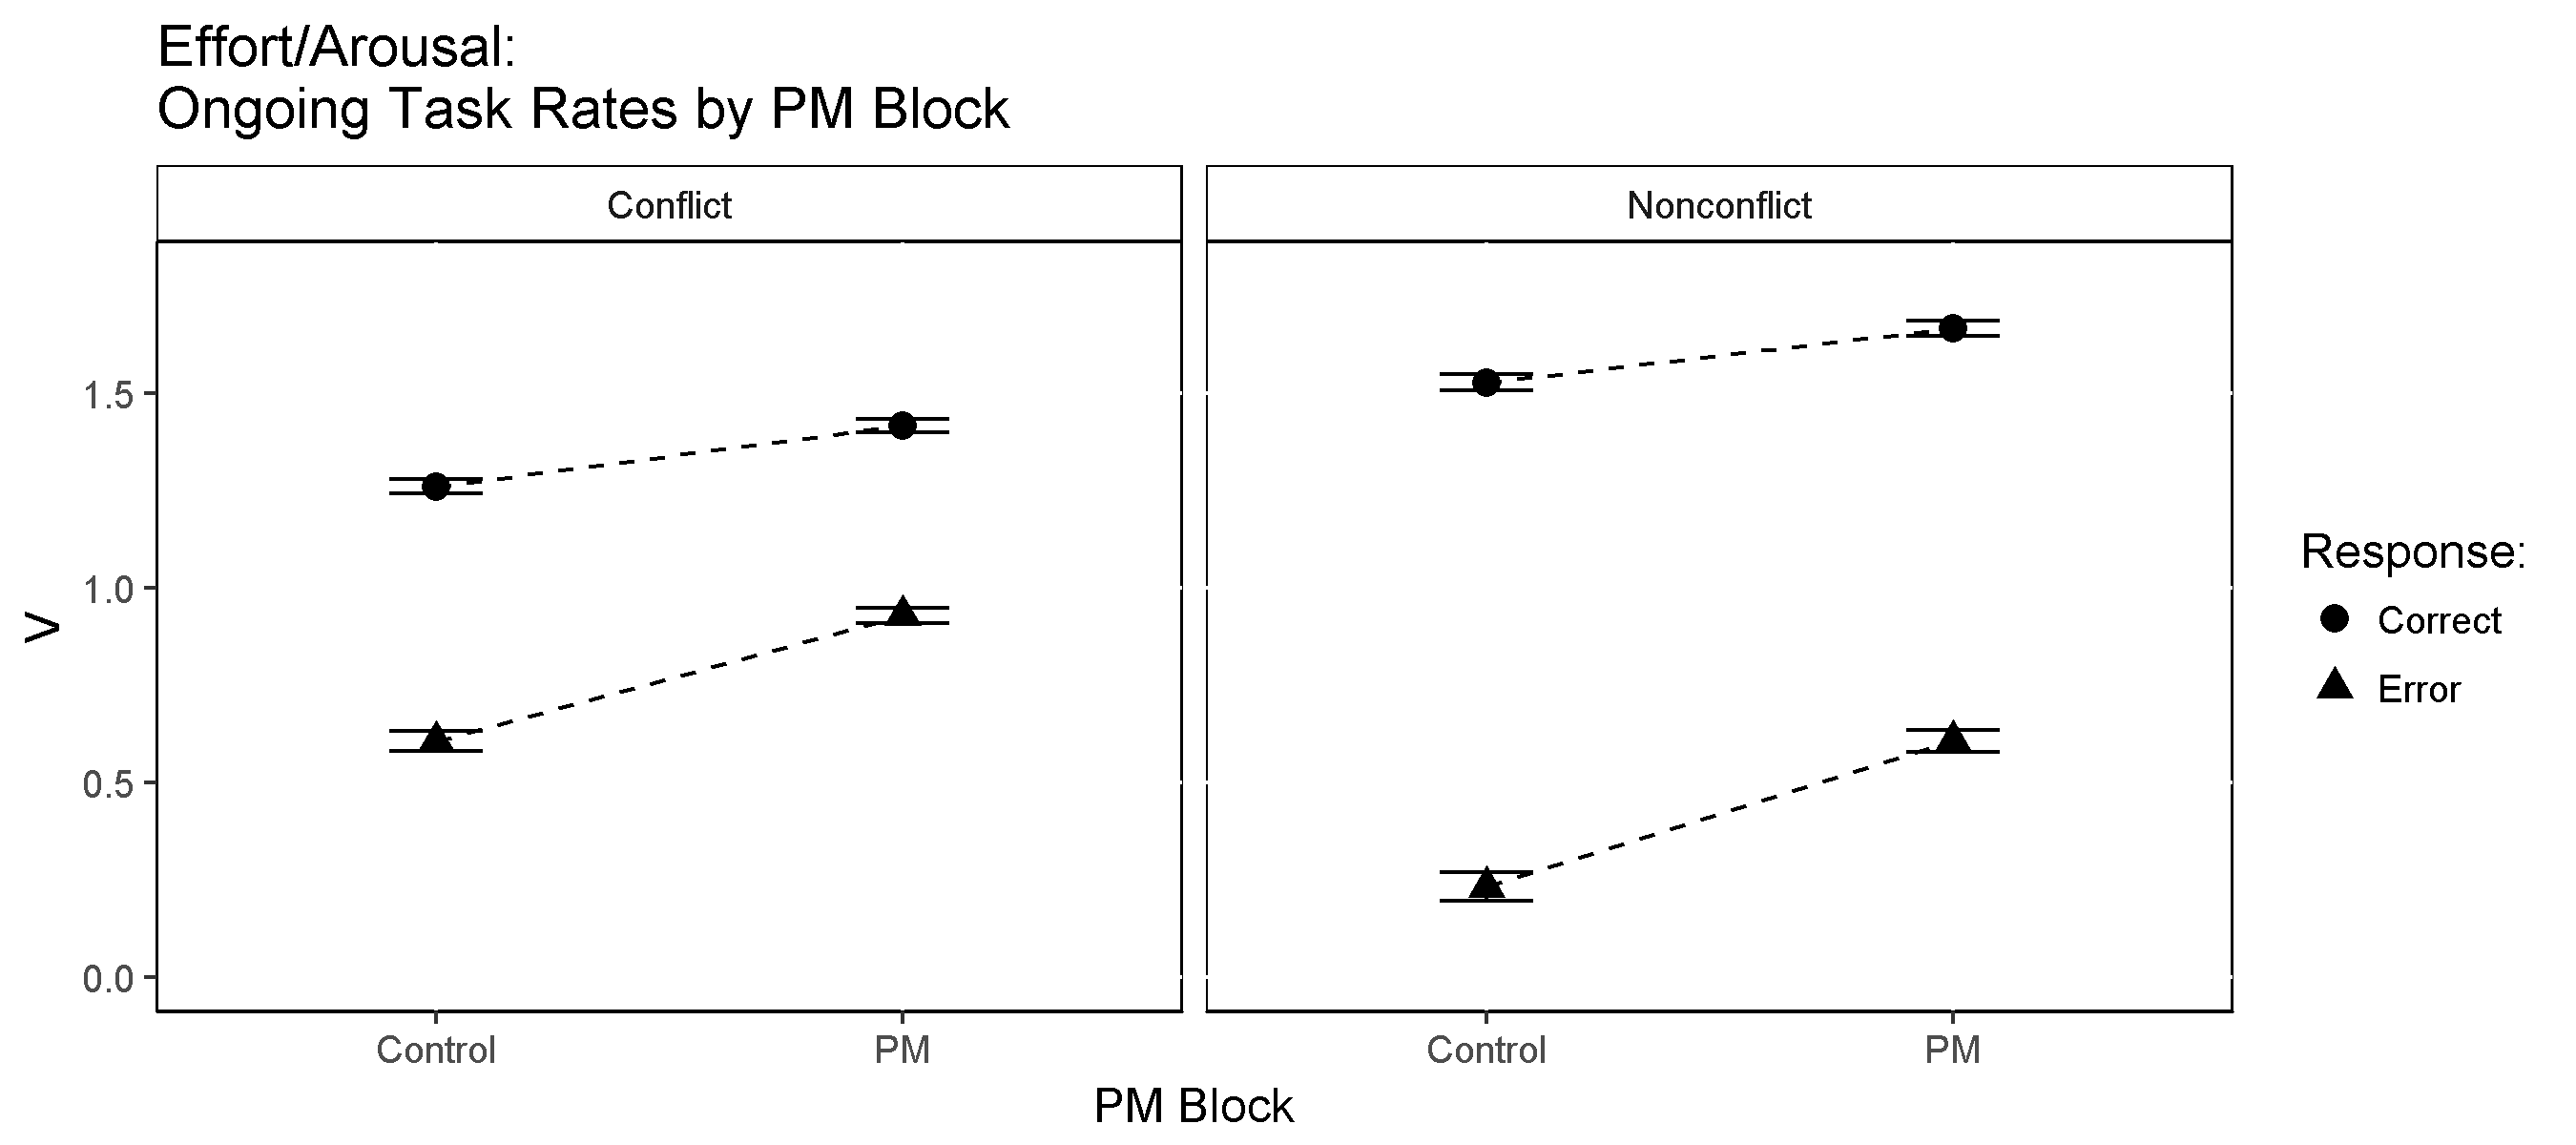
\includegraphics[width=0.8\linewidth]{figures/E1/E1.Effort.Arousal.PM} \caption{\label{fig:Effort.Arousal.PM}Ongoing Task Accumulation Rates by PM Block. Central symbols represent posterior means. Error bars represent +/- 1 posterior standard deviation.}\label{fig:Plot: Capacity PM}
\end{figure}

\subsubsection{Proactive Control
(Thresholds)}\label{proactive-control-thresholds}

\paragraph{Proactive Control under PM
Demand}\label{proactive-control-under-pm-demand}

PM cost theories that involve proactive control over ongoing task
decisions (e.g., strategic delay theory) predict higher conflict and
nonconflict response thresholds under PM load compared to during control
blocks. Figure \ref{fig:Proactive.Control.PM} shows conflict and
nonconflict response thresholds in the control and PM blocks.
\emph{Z}-score effect sizes and p-values for threshold comparisons are
shown in Table XX in the supplementary materials.

As Figure \ref{fig:Proactive.Control.PM} shows, ongoing task thresholds
were much higher in PM than control blocks for both conflict (\emph{Z} =
35.17, \emph{p} = 0) and nonconflict (\emph{Z} = 44.12, \emph{p} = 0)
responses. This is consistent with strategic delay theories of PM costs
whereby responses to the ongoing task are deliberately delayed in order
to avoid preempting PM targets.

\begin{figure}
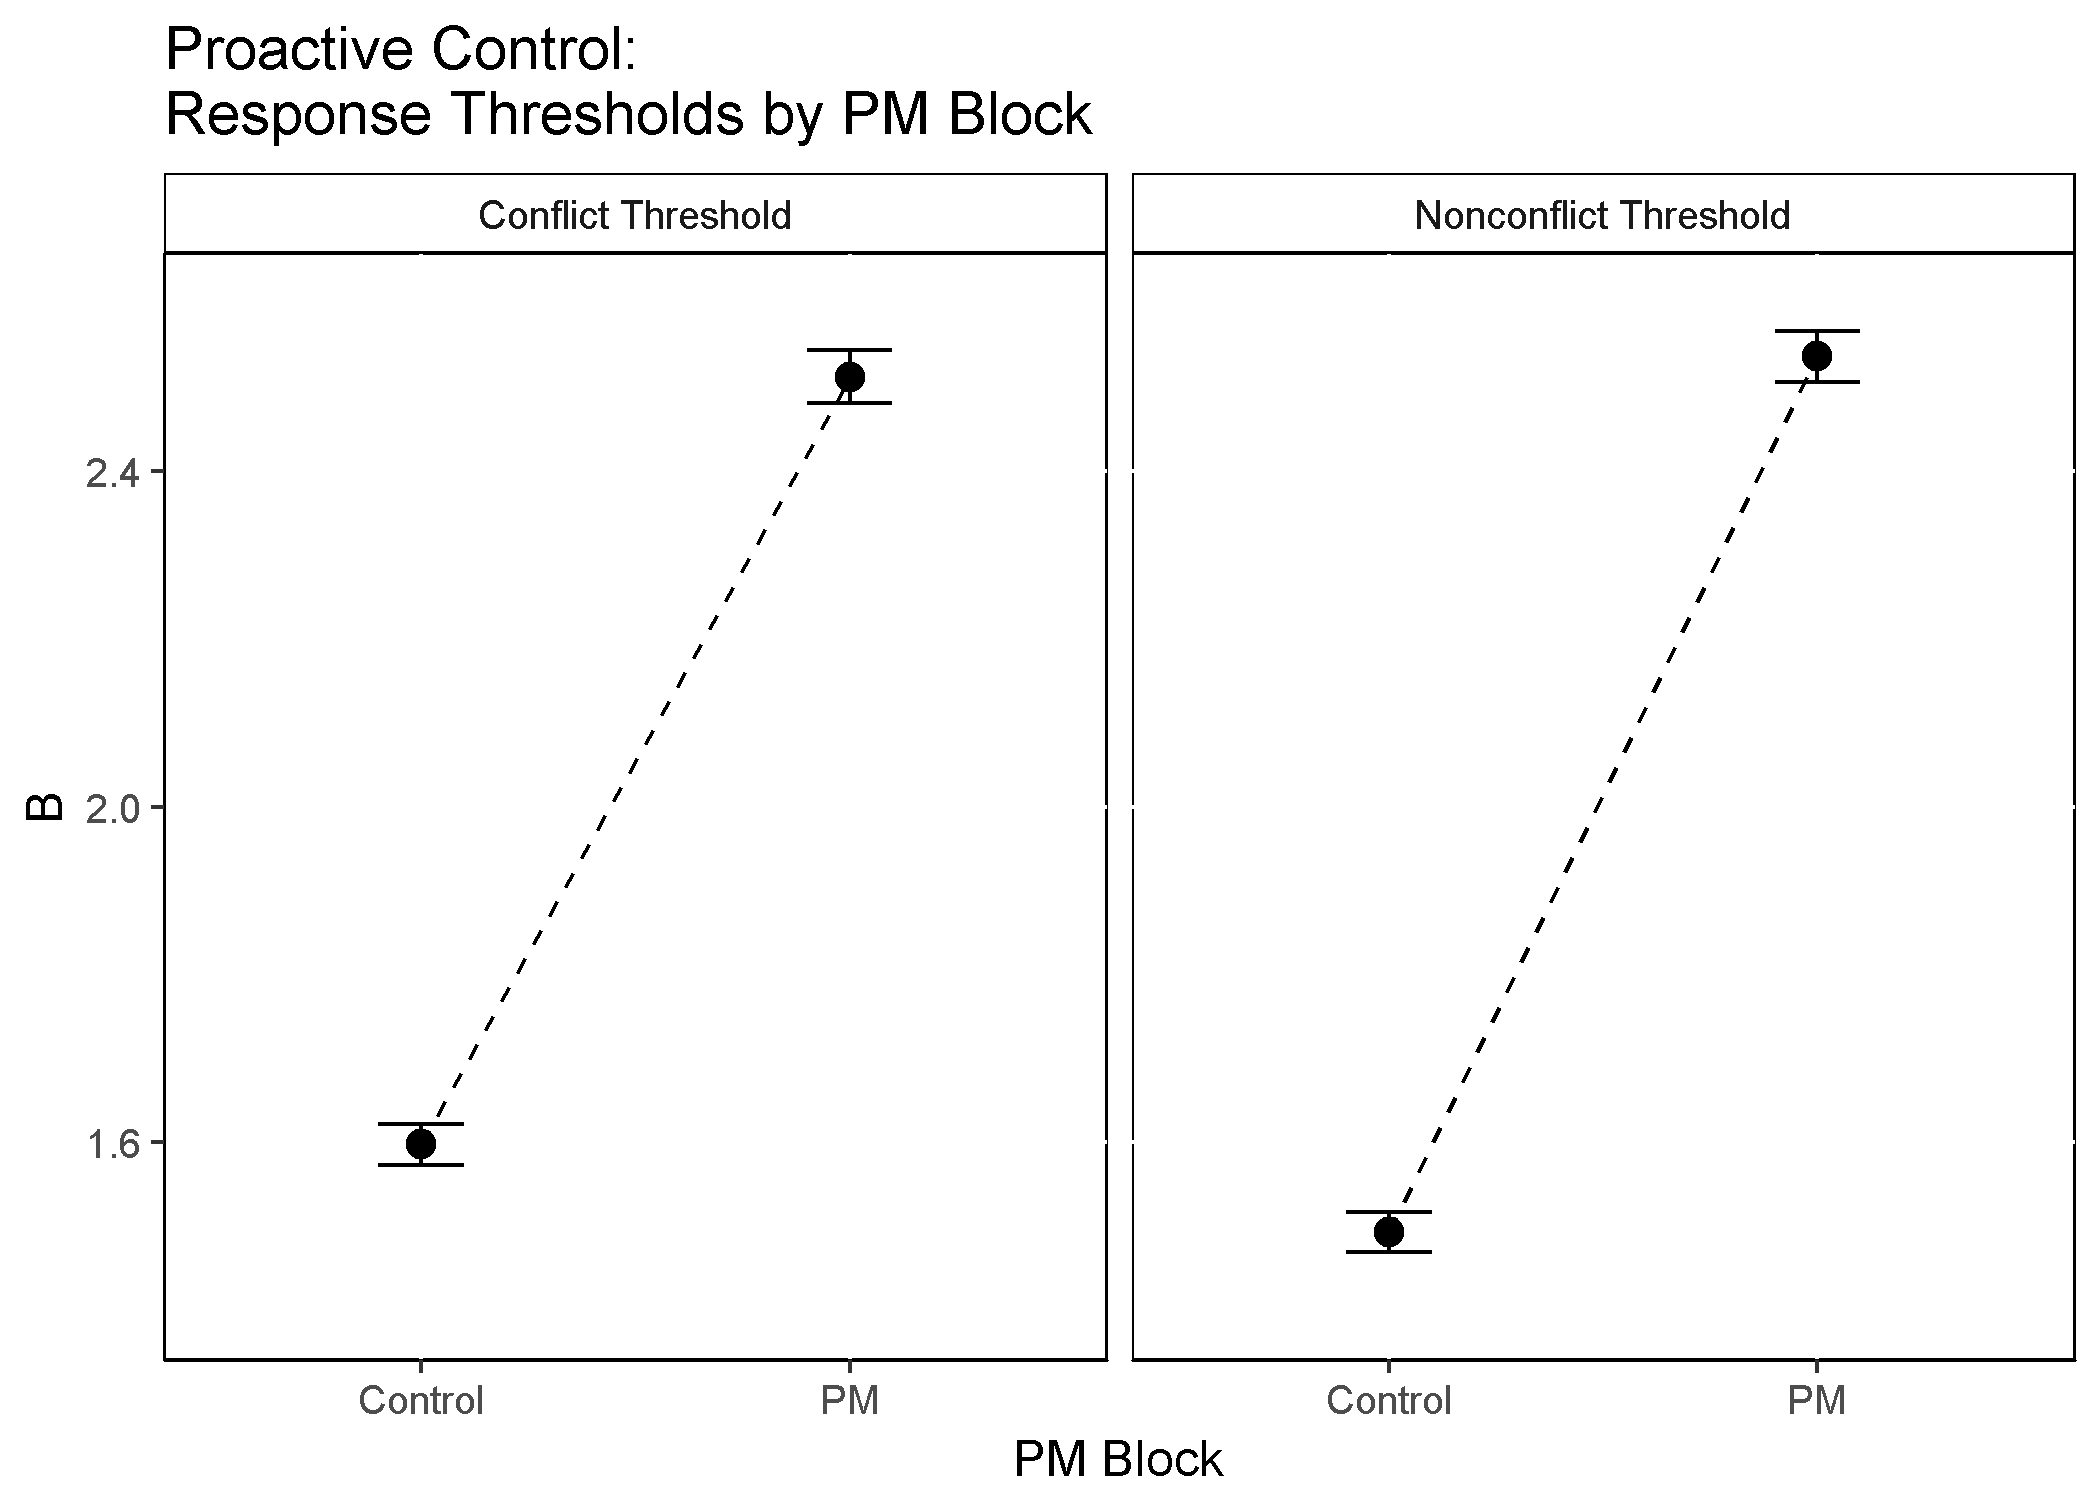
\includegraphics[width=0.8\linewidth]{figures/E1/E1.Proactive.Control.PM} \caption{\label{fig:Proactive.Control.PM}Ongoing Task Thresholds by PM Block. Central symbols represent posterior means. Error bars represent +/- 1 posterior standard deviation.}\label{fig:Plot: Proactive Control PM}
\end{figure}

\paragraph{Proactive Control under Time
Pressure}\label{proactive-control-under-time-pressure}

A common finding in decision-making literature is that of the
speed-accuracy trade-off, in which individuals can deliberately increase
the speed of their responses (at the expense of accuracy) or increase
the accuracy of their responses (at the expense of speed). Several
choice-RT modelling studies have shown these effects are well acounted
for by strategic threshold adjustments (i.e., proactive control) in
response to different levels of time pressure or speed/accuray emphasis.
Figure \ref{fig:Proactive.Control.TP} shows ongoing task and PM response
thresholds under low and high time pressure for both low trial load (2
decisions per trial) and high trial load (5 decisions per trial).
\emph{Z}-score effect sizes and \emph{p} values are shown in Table XX in
the supplementary materials.

As shown in Figure \ref{fig:Proactive.Control.TP}, control block ongoing
task thresholds decreased under high time pressure relative to low time
pressure during both low trial load (\emph{Z} = 7.14, \emph{p} = 0) and
high trial load (\emph{Z} = 7.79, \emph{p} = 0) conditions. Similarly,
PM block ongoing task thresholds decreased under high time pressure
relative to low time pressure during both low trial load (\emph{Z} =
14.39, \emph{p} = 0) and high trial load (\emph{Z} = 23.73, \emph{p} =
0) conditions. Ongoing task thresholds also decreased between low and
high trial load with time pressure held constant (Control: \emph{Z} =
2.24, \emph{p} = .013; PM: \emph{Z} = 2.65, \emph{p} = .004). PM
response thresholds also decreased under high time pressure relative to
low time pressure during both low trial load (\emph{Z} = 7.97, \emph{p}
= 0) and high trial load (\emph{Z} = 9.86, \emph{p} = 0), but did not
differ by trial load. This is consistent with much choice-RT modelling
of the speed-accuracy trade-off and supports a proactive control account
in which thresholds are strategically lowered to facilitate fast
responding (at the expense of accuracy).

In addition to strategic threshold shifts in response to increased time
pressure, time pressure also interacted with proactive control PM cost
effects. Specifically, the magnitude of strategic threshold adjustments
between control and PM blocks was attenuated under high time pressure
conditions compared to low time pressure conditions. As shown in Table
XX, the magnitude of PM-Control threshold differences decreased under
high time pressure relative to low time pressure during both low trial
load (\emph{Z} = 4.83, \emph{p} = 0) and high trial load (\emph{Z} =
11.58, \emph{p} = 0). The magnitude of PM-Control threshold differences
was unaffected by trial load for both conflict and nonconflict
responses. Taken together, and considering the very large magnitude of
the effects, these threshold shifts in response to changes in both PM
demand and time pressure provide convincing evidence that proactive
control via strategic threshold adjustment is an important driver of
observed PM cost and speed-accuracy trade-off effects.

\begin{figure}
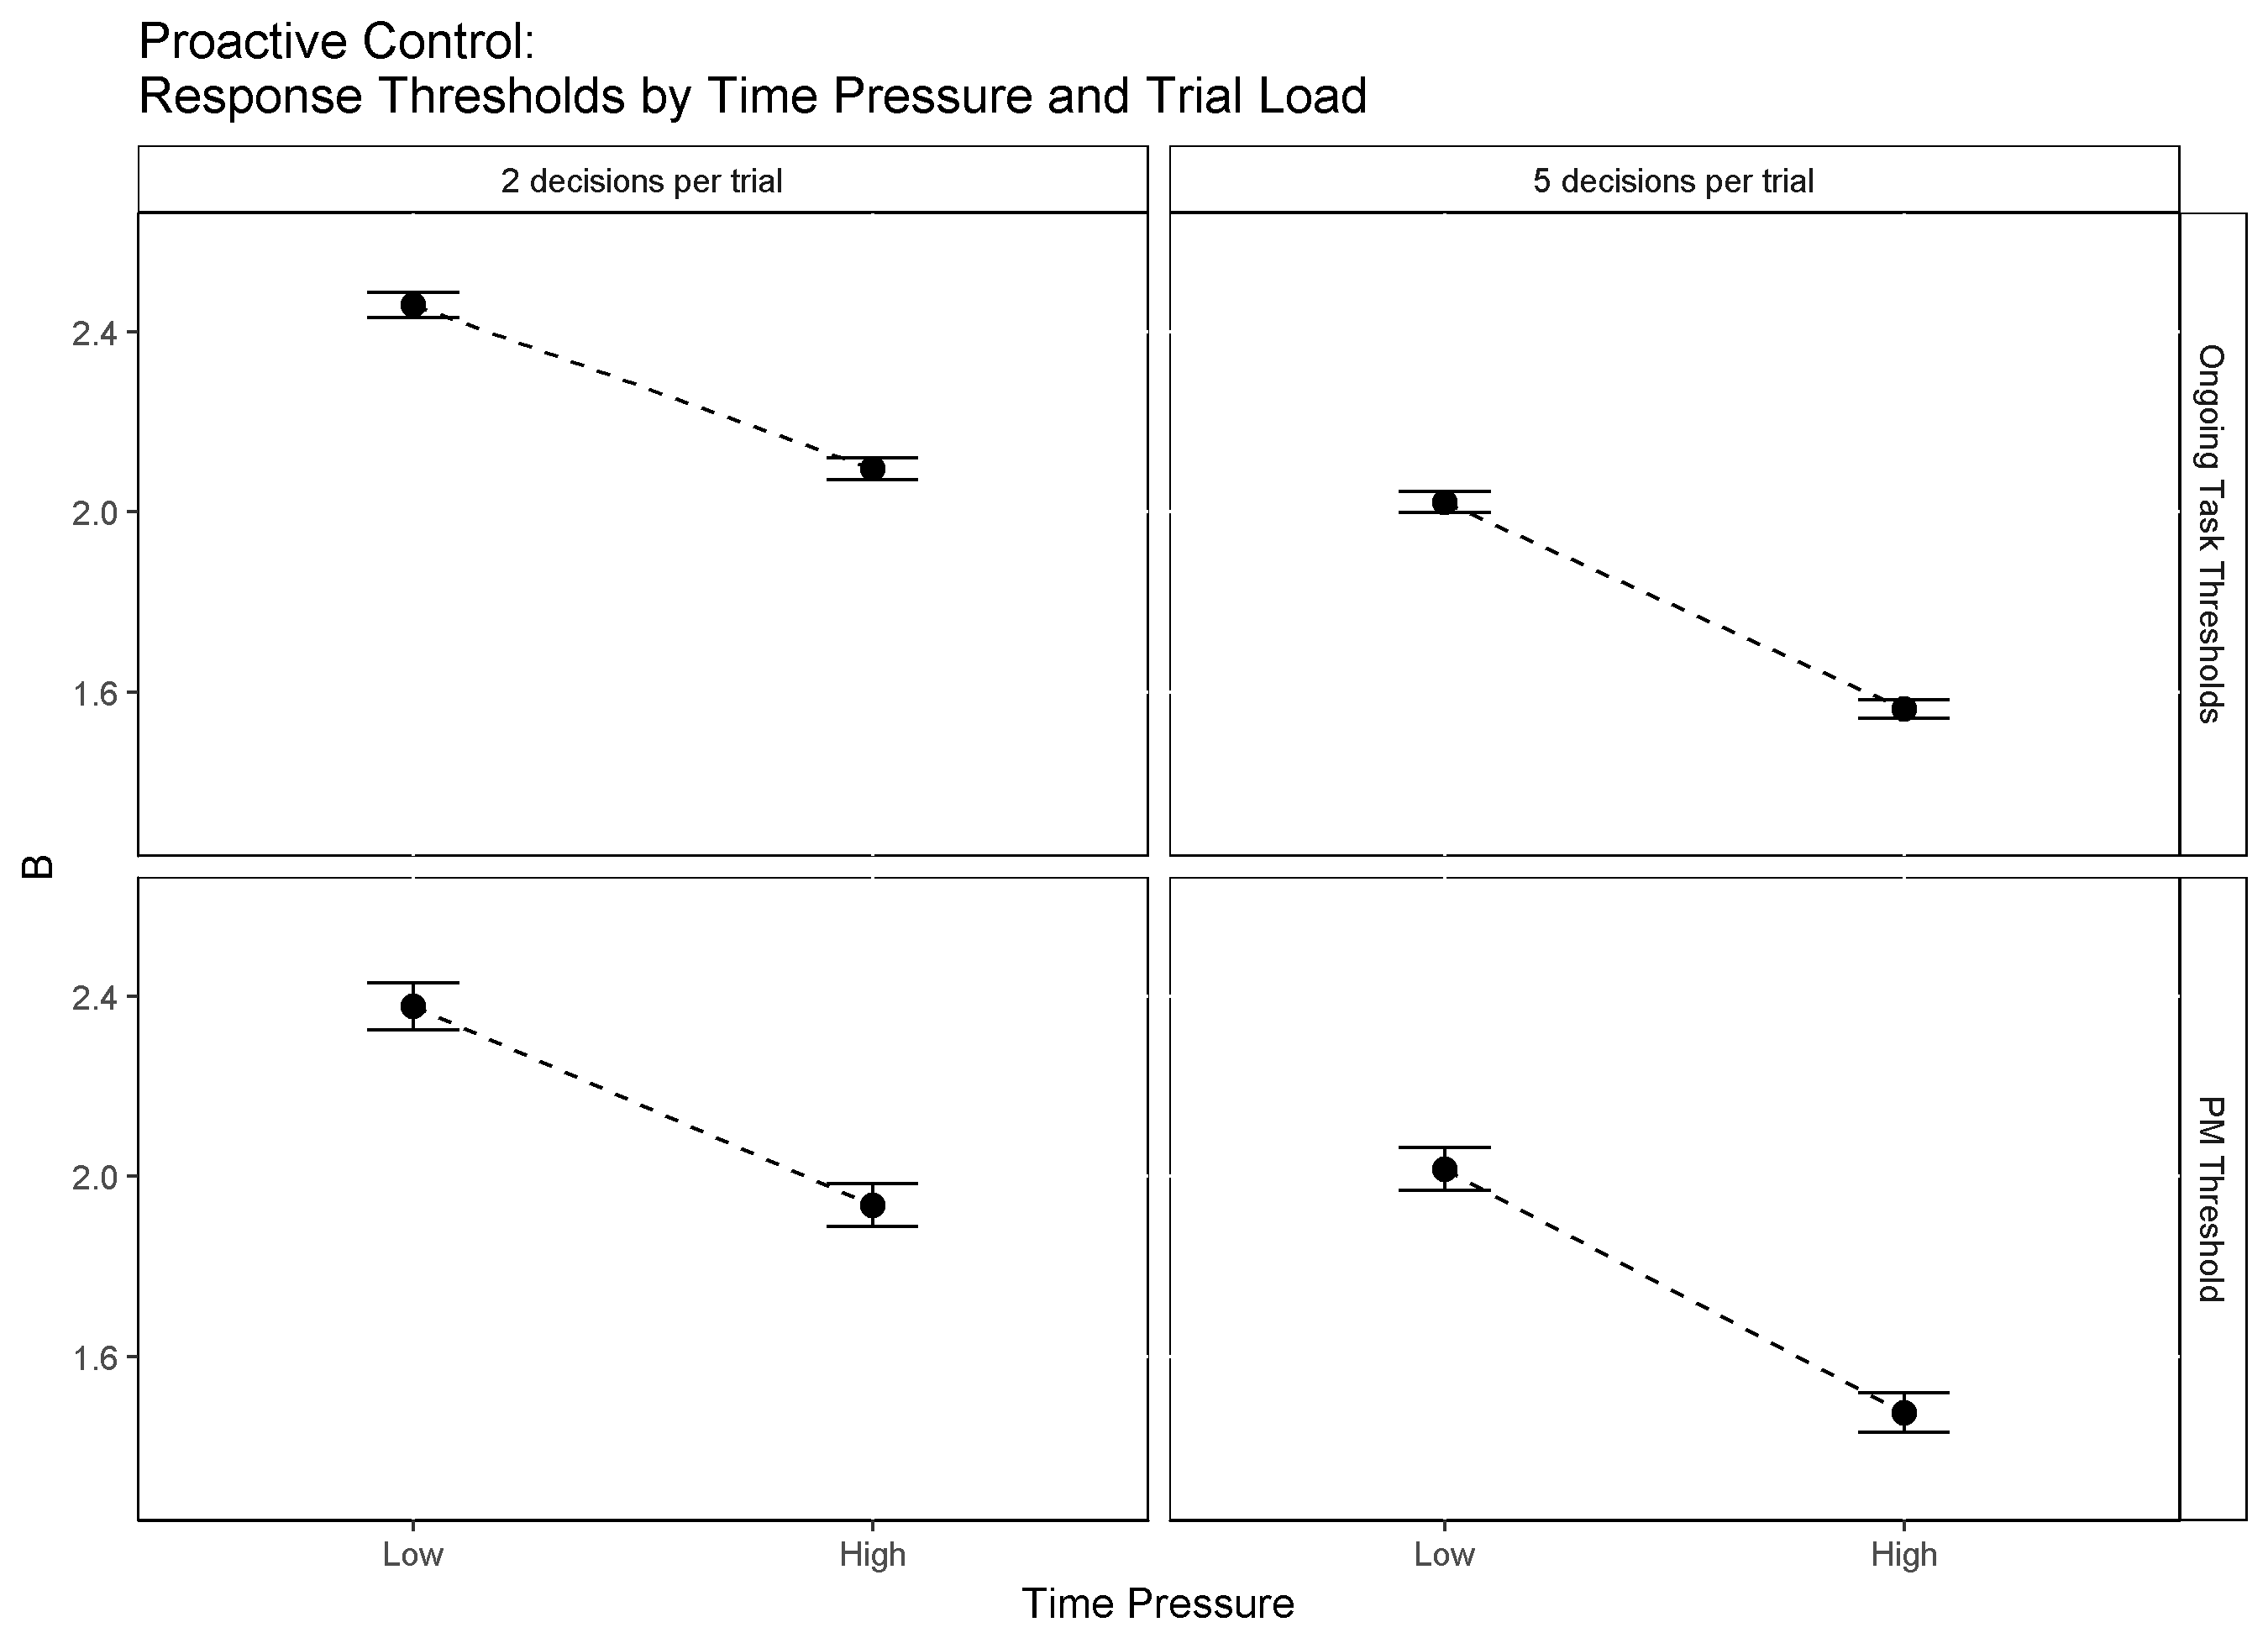
\includegraphics[width=0.8\linewidth]{figures/E1/E1.Proactive.Control.TP} \caption{\label{fig:Proactive.Control.TP}Ongoing Task and PM Thresholds by Time Pressure. Central symbols represent posterior means. Error bars represent +/- 1 posterior standard deviation.}\label{fig:Plot: Proactive Control TP}
\end{figure}

\subsubsection{Reactive Inhibition (PM vs.~Non-PM Trial
Accumulation)}\label{reactive-inhibition-pm-vs.non-pm-trial-accumulation}

A prediction of PMDC theory is that ongoing task (conflict/nonconflict)
evidence accumulation rates will be lower on PM trials due to `reactive'
or stimulus-driven inhibitory control of the decision process by the PM
stimulus detector. Figure \ref{fig:Reactive.Inhibition} shows
accumulation rates for ongoing task responses to non-PM
conflict/nonconflict stimuli compared to PM conflict/nonconflict stimuli
(i.e., ongoing task stimuli that also contained a PM target).
\emph{Z}-score effect sizes and \emph{p} values are shown in Table XX in
the supplementary materials.

Consistent with the predictions of PMDC's reactive inhibition mechanism,
rates for ongoing task accumulators where much lower for stimuli
containing a PM cue compared to when the same stimuli did not contain a
PM cue (Conflicts: \emph{Z} = 13.26, \emph{p} = 0; Nonconflicts:
\emph{Z} = 12.63, \emph{p} = 0). This supports the idea that when the PM
detector detects a PM target, the accumulation process for the competing
ongoing task response is supressed or inhibited.

Moreover, the magnitude of reactive inhibition for ongoing task
responses was generally stronger for the correct response accumulators
(\emph{Z} = 18.09, \emph{p} = 0) compared to error response accumulators
(\emph{Z} = 15.3, \emph{p} = 0). This suggests that response inhibition
processes are somewhat stimulus-specific or targeted toward the specific
ongoing task response currently competing with the PM accumulator for
selection.

These findings are consistent with the idea that response accumulators
compete with each other based on their inputs; in the presence of a PM
stimulus, evidence accumulation processes for conflicts and nonconflicts
are inhibited relative to when a PM stimulus is absent. Moreover, the
stronger inhibition of congruent ongoing task accumulators suggests that
reactive inhibition processes may selectively inhibit more salient
competing responses.

\begin{figure}
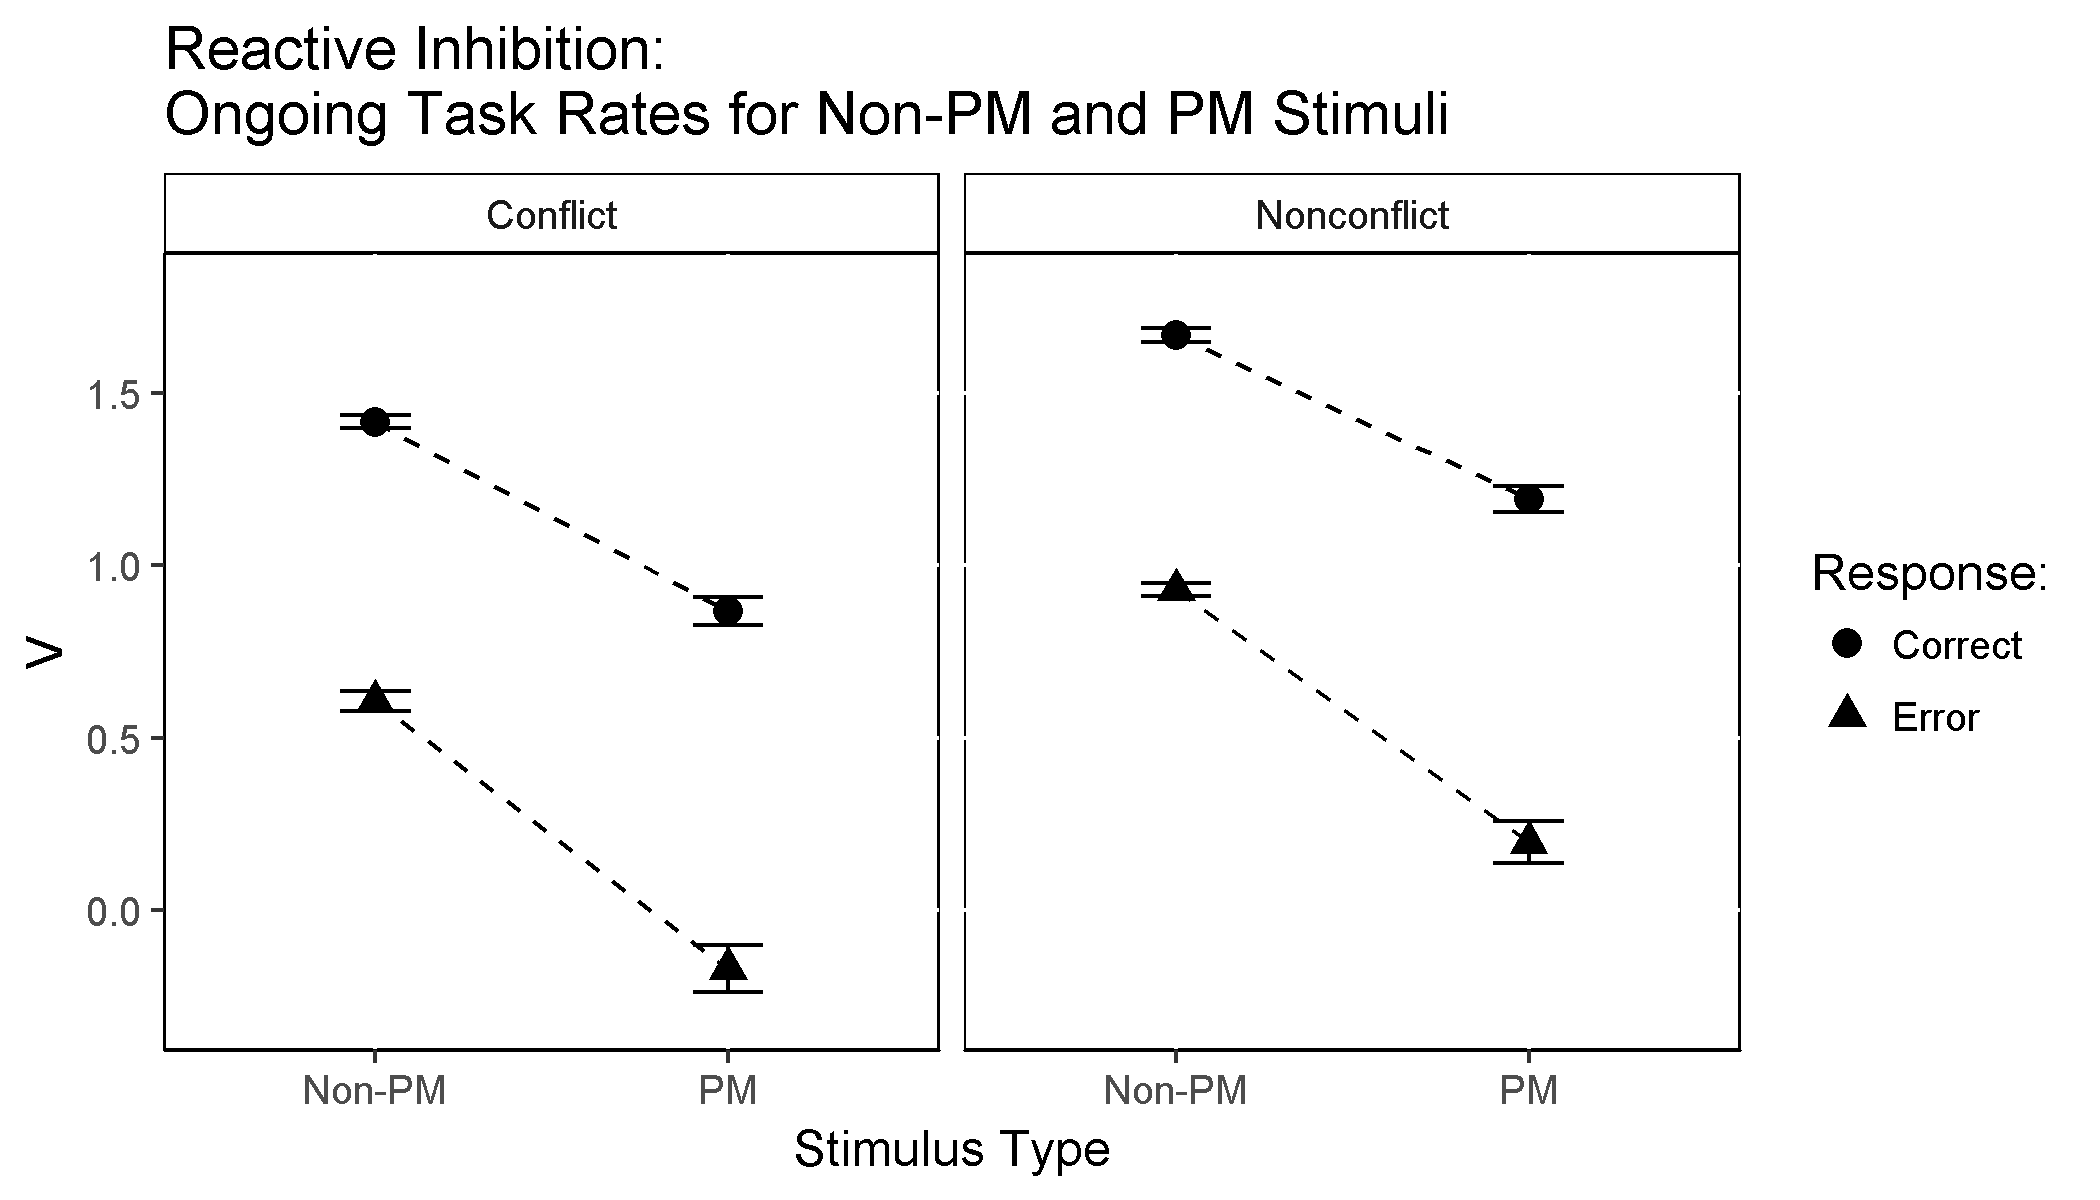
\includegraphics[width=0.8\linewidth]{figures/E1/E1.Reactive.Inhibition} \caption{\label{fig:Reactive.Inhibition}Ongoing Task Accumulation Rates for PM and Non-PM Stimuli. Central symbols represent posterior means. Error bars represent +/- 1 posterior standard deviation.}\label{fig:Plot: Reactive Inhibition}
\end{figure}

\subsubsection{Effort/Arousal (Accumulation Rate Increases with PM Load
and Time
Pressure)}\label{effortarousal-accumulation-rate-increases-with-pm-load-and-time-pressure}

As mentioned previously, in contrast with the predictions of
capacity-sharing theories of PM costs, we found that evidence
accumulation rates actually increased with the addition of PM load.
Figure \ref{fig:Effort.Arousal.TP} shows correct and error accumulation
rates across the different levels of time pressure for both low trial
load (2 decisions per trial) and high trial load (5 decisions per trial)
conditions. \emph{Z}-score effect sizes and \emph{p} values are shown in
Table XX in the supplementary materials.

As with the increases seen from control to PM blocks, accumulation rates
for correct ongoing task repsonses were higher in high time pressure
blocks during both low trial load (\emph{Z} = -11.33, \emph{p} = 0) and
high trial load (\emph{Z} = -24.11, \emph{p} = 0). Similarly,
accumulation rates for ongoing task errors were also higher in high time
pressure blocks during both low trial load (\emph{Z} = -11.93, \emph{p}
= 0) and high trial load (\emph{Z} = -24.0, \emph{p} = 0).

Since rates for both correct and error responses increase with time
pressure, this effect is suggestive of an overall increase in
arousal/task engagement or the overall effort being invested in
completing the task. One possible explanation is that the task becomes
more difficult or engaging under high time pressure leading participants
to deploy more cognitive resources toward completing the task.

Alternatively, rather than increasing effort in response to greater
difficulty, participants could be `satisficing', or decreasing effort
when the task is perceived as easy. For example, in the relatively easy
control and low time pressure conditions participants may believe that
they can disengage from the task somewhat, expending fewer cognitive
resources while still maintaining a satisfactory level of task
performance.

Several additional lines of evidence support this effort/task engagement
hypothesis. First, both PM block and time pressure were highly
significant predictors of self-reported effort ratings on the NASA-TLX
(see Table XX in the supplementary materials); participants reported
expending more effort under PM load compared to control as well as
expending more effort during higher time pressure blocks. Planned
comparisons revealed that effort increased significantly with time
pressure during both low trial load (\emph{t} = -3.44, \emph{df} = 93,
\emph{p} = 0.001, \emph{Cohen's d} = 0.35, and high trial load
conditions (\emph{t} = -8.45, \emph{df} = 93, \emph{p} =
\textless{}0.001, \emph{Cohen's d} = 0.87. Second, ongoing task
accumulation rates were significant predictors of self-reported effort
ratings (see Table XX in the supplementary materials). Specifically,
rates for both conflict and nonconflict error accumulators were positive
predictors of effort, whereas correct accumulation rates were not.

As such, it seems as though subjects can choose to deploy more cognitive
resources into the task when changes in environmental conditions such as
PM load and time pressure suggest it may be advantageous to do so.
Crucially, such resources need not be diverted from the ongoing task,
contrary to the claims of capacity-sharing explanations. However, it is
interesting to note that error accumulation rates for the ongoing task
were more related to effort ratings than were correct accumulation
rates. This suggests that although subjects can increase their arousal
or exert more effort, that extra effort or arousal may not necessarily
translate into higher quality information processing.

\begin{figure}
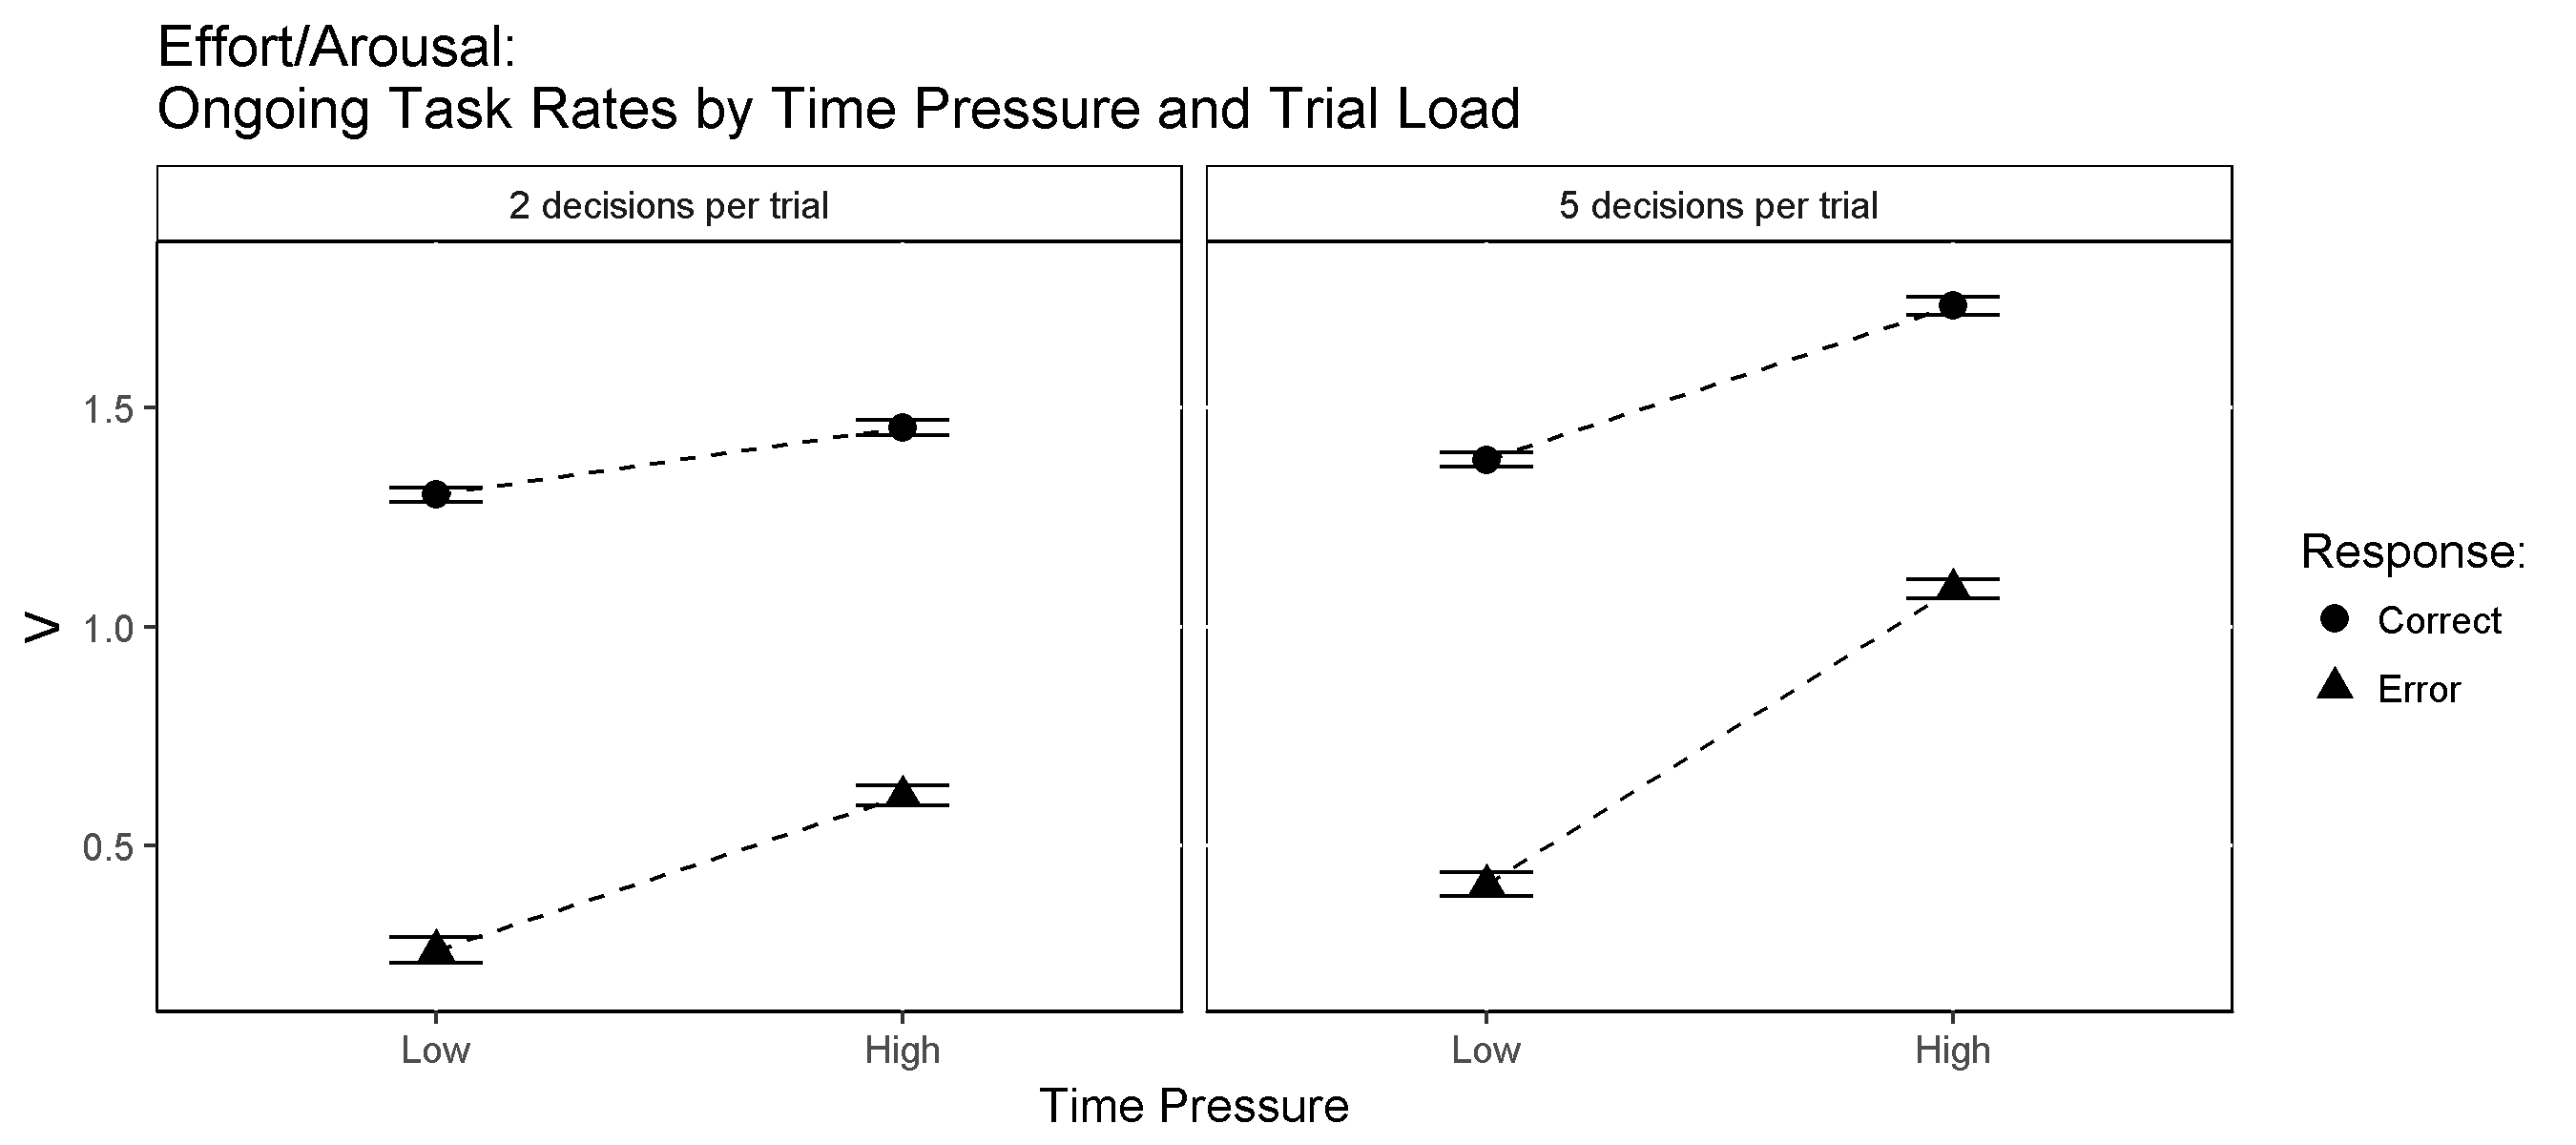
\includegraphics[width=0.8\linewidth]{figures/E1/E1.Effort.Arousal.TP} \caption{\label{fig:Effort.Arousal.TP}Ongoing Task Accumulation Rates by Time Pressure. Central symbols represent posterior means. Error bars represent +/- 1 posterior standard deviation.}\label{fig:Plot: Effort/Arousal}
\end{figure}

\subsection{Model Exploration}\label{model-exploration}

Given the complexity of our model, it is difficult to discern the
overall contribution given parameters have on overall RT and/or
accuracy. In this section we attempt to tease out the individual
contribution to RT and accuracy provided by certain parameters and
mechanisms in the model. It is our aim to give a clearer picture of the
relative importance of key parameters in accounting for the observed
effects.

In order to evaluate a given parameter's contribution to the model, we
first replace that parameter with the average either across control/PM
blocks or across time pressure levels (e.g., replacing control and PM
ongoing task thresholds with the average of the two). We can then
examine the associated mis-fit of the model with the removed effect
relative to the full model with the effect included.

We generated posterior predictions for all of the PM and time pressure
effects for the selected model, and then separately for models with two
different sets of parameters averaged over either PM or time pressure
blocks: ongoing accumulation rates, and ongoing thresholds.

In the supplementary materials, we include fit graphs comparing the full
model to the two versions with proactive (threshold) and reactive (rate)
mechanisms systematically turned off.

Here we focus our discussion on PM cost and time pressure effects and
the contribution of each cognitive mechanism toward explaining the
effects. First, we assess how much of the PM accuracy and RT effects
were accounted for by the different models, and whether each model
adequately fit these effects. Second, we assess how much of the time
pressure accuracy and RT effects were accounted for by the different
models, and whether each model adequately fit these effects. Finally, we
examine the penalty associated with selectively turning off proactive
control mechanisms, reactive inhibition mechanisms, or both in terms of
fit to overall accuracy and RT.

\subsubsection{PM Cost Effects}\label{pm-cost-effects}

As shown in Figure \ref{fig:PM.Control.Contrast.Plots}, the full
(selected) model accounted for the accuracy and RT costs associated with
PM demand fairly well, providing close fits to the difference between
control and PM accuracy for both conflict and nonconflict stimuli, and
closely fit the cost to both correct and error RT for both ongoing task
responses.

Averaging the ongoing task thresholds between control and PM blocks made
the model overpredict the cost to ongoing task accuracy, more so for
conflicts than nonconflicts, and dramatically underpredict the cost to
both correct and error ongoing task RT (so much so that the model in
fact predicted a PM advantage to ongoing task RT rather than a cost).
This further indicates that proactive control of thresholds is an
important mechanism in explaining PM costs effects, in particular costs
to ongoing task RT.

In contrast, averaging the ongoing task accumulation rates between
control and PM blocks caused the model to underpredict costs to ongoing
task accuracy (predicting an accuracy advantage for conflicts) and
overpredict costs to both correct and error ongoing task RT. This
suggests that reactive inhibition of accumulation rates is also an
important mechanism in explaining the differences in ongoing task
accuracy and RT that occur under PM demand.

\subsubsection{Time Pressure Effects}\label{time-pressure-effects}

In terms of time pressure effects, the full model provided a very close
account of accuracy differences between low and high time pressure
blocks under both low and high trial load conditions (Figure
\ref{fig:ModelExpTPContrastsOngoing}). The full model also closely fit
RT differences between time pressure blocks for both correct and error
ongoing task responses as well as PM responses.

Averaging the ongoing task thresholds made the model overpredict the
cost to ongoing task accuracy under increased time pressure for
conflcits, that is, it predicted lower conflict accuracy in the high
time pressure blocks than was observed. Conversely, the model
underpredicted the cost to ongoing task accuracy under increased time
pressure for nonconflcits, that is, it predicted higher nonconflict
accuracy in the high time pressure blocks than was observed.

Similarly, the averaged-threshold model underpredicted RT differences
between high and low time pressure blocks for both correct and error
conflict and nonconflict responses (i.e., it predicted less of a
speed-up from low to high time pressure than was observed). This
provides further evidence that proactive control mechanisms are critical
for explaining empirical speed-accuracy trade-off effects under
different levels of time pressure.

Averaging the ongoing task accumulation rates resulted in a model that
underpredicts the cost to ongoing task accuracy under increased time
pressure (actually predicting an accuracy advantage for conflicts under
high time pressure instead of the observed cost). Likewise, the
averaged-rates model underpredicts RT differences between high and low
time pressure blocks for both correct and error conflict and nonconflict
responses, predicteding less of a speed-up from low to high time
pressure than was observed.

In terms of PM responses, the averaged-threshold model maintained close
fits to PM accuracy, but severely underpredicted RT differences between
high and low time pressure blocks. In contrast, the averaged-rates model
maintained close fits with PM RT, but underpredicted accuracy
differences between high and low time pressure blocks (i.e., predicted
higher PM accuracy under high time pressure than was observed). Taken
together, both proactive and reactive control mechanisms appear
necessary to account for the full range of RT and accuracy differences
under different levels of time pressure.

\subsubsection{Importance of Cognitive Control
Mechanisms}\label{importance-of-cognitive-control-mechanisms}

Finally, we examine the overall importance of proactive and reactive
inhibition mechanisms in terms of how well the model fits observed
accuracy and RT. As shown in Figure
\ref{fig:ModelExpTPContrastsPM_ControlMech}, the full model (which
includes both proactive and reactive control mechanisms) provided an
almost exact fit to accuracy (99.91\% of the effect), while slightly
overpredicting overall RT (RT overpredicted by 1.34\%).

In contrast, when proactive control is removed and the model only allows
for reactive control, we get severe mis-fit to both overall accuracy and
RT, the model underpredicting both by a large margin (accuracy
underpredicted by 17.48\%, RT underpredicted by 8.77\%). Similarly, when
reactive control is removed from the model and only proactive control
included, we get less severe but still substantial underprediction of
both accuracy and RT (accuracy underpredicted by 9.46\%, RT
underpredicted by 4.11\%).

Lastly, when both proactive and reactive control mechanisms are turned
off (i.e., the model includes neither mechanism), the model produces the
worst overall fit to accuracy and RT, underpredicting both by a larger
margin than either the proactive-only or reactive-only models (accuracy
underpredicted by 30.25\%, RT underpredicted by 15.64\%). This provides
convincing evidence that both proactive and reactive control mechanisms
play critical and complimentary roles in accounting for ongoing task
costs associated with different PM and time pressure demands.

\section{Supplementary Materials}\label{supplementary-materials}

\begin{longtable}[]{@{}lrrr@{}}
\caption{Significance testing linear predictors of ongoing task
accuracy. Accuracies were analysed with a generalised linear model with
a binomial probit link function which predicts the outcome of every
trial. Tests for significance use Wald's chi-square test with an alpha
level of .05.}\tabularnewline
\toprule
\begin{minipage}[b]{0.36\columnwidth}\raggedright\strut
Factor\strut
\end{minipage} & \begin{minipage}[b]{0.16\columnwidth}\raggedleft\strut
Chi-square\strut
\end{minipage} & \begin{minipage}[b]{0.06\columnwidth}\raggedleft\strut
df\strut
\end{minipage} & \begin{minipage}[b]{0.06\columnwidth}\raggedleft\strut
p\strut
\end{minipage}\tabularnewline
\midrule
\endfirsthead
\toprule
\begin{minipage}[b]{0.36\columnwidth}\raggedright\strut
Factor\strut
\end{minipage} & \begin{minipage}[b]{0.16\columnwidth}\raggedleft\strut
Chi-square\strut
\end{minipage} & \begin{minipage}[b]{0.06\columnwidth}\raggedleft\strut
df\strut
\end{minipage} & \begin{minipage}[b]{0.06\columnwidth}\raggedleft\strut
p\strut
\end{minipage}\tabularnewline
\midrule
\endhead
\begin{minipage}[t]{0.36\columnwidth}\raggedright\strut
Stimulus\strut
\end{minipage} & \begin{minipage}[t]{0.16\columnwidth}\raggedleft\strut
1121\strut
\end{minipage} & \begin{minipage}[t]{0.06\columnwidth}\raggedleft\strut
1\strut
\end{minipage} & \begin{minipage}[t]{0.06\columnwidth}\raggedleft\strut
\textless{}.001\strut
\end{minipage}\tabularnewline
\begin{minipage}[t]{0.36\columnwidth}\raggedright\strut
PM Block\strut
\end{minipage} & \begin{minipage}[t]{0.16\columnwidth}\raggedleft\strut
13.61\strut
\end{minipage} & \begin{minipage}[t]{0.06\columnwidth}\raggedleft\strut
1\strut
\end{minipage} & \begin{minipage}[t]{0.06\columnwidth}\raggedleft\strut
\textless{}.001\strut
\end{minipage}\tabularnewline
\begin{minipage}[t]{0.36\columnwidth}\raggedright\strut
Time Pressure\strut
\end{minipage} & \begin{minipage}[t]{0.16\columnwidth}\raggedleft\strut
343.3\strut
\end{minipage} & \begin{minipage}[t]{0.06\columnwidth}\raggedleft\strut
3\strut
\end{minipage} & \begin{minipage}[t]{0.06\columnwidth}\raggedleft\strut
\textless{}.001\strut
\end{minipage}\tabularnewline
\begin{minipage}[t]{0.36\columnwidth}\raggedright\strut
Stimulus by PM Block\strut
\end{minipage} & \begin{minipage}[t]{0.16\columnwidth}\raggedleft\strut
3.37\strut
\end{minipage} & \begin{minipage}[t]{0.06\columnwidth}\raggedleft\strut
1\strut
\end{minipage} & \begin{minipage}[t]{0.06\columnwidth}\raggedleft\strut
.0664\strut
\end{minipage}\tabularnewline
\begin{minipage}[t]{0.36\columnwidth}\raggedright\strut
Stimulus by Time Pressure\strut
\end{minipage} & \begin{minipage}[t]{0.16\columnwidth}\raggedleft\strut
64.9\strut
\end{minipage} & \begin{minipage}[t]{0.06\columnwidth}\raggedleft\strut
3\strut
\end{minipage} & \begin{minipage}[t]{0.06\columnwidth}\raggedleft\strut
\textless{}.001\strut
\end{minipage}\tabularnewline
\begin{minipage}[t]{0.36\columnwidth}\raggedright\strut
PM Block by Time Pressure\strut
\end{minipage} & \begin{minipage}[t]{0.16\columnwidth}\raggedleft\strut
13.67\strut
\end{minipage} & \begin{minipage}[t]{0.06\columnwidth}\raggedleft\strut
3\strut
\end{minipage} & \begin{minipage}[t]{0.06\columnwidth}\raggedleft\strut
.0034\strut
\end{minipage}\tabularnewline
\begin{minipage}[t]{0.36\columnwidth}\raggedright\strut
Stimulus by PM Block by Time Pressure\strut
\end{minipage} & \begin{minipage}[t]{0.16\columnwidth}\raggedleft\strut
4.59\strut
\end{minipage} & \begin{minipage}[t]{0.06\columnwidth}\raggedleft\strut
3\strut
\end{minipage} & \begin{minipage}[t]{0.06\columnwidth}\raggedleft\strut
.2045\strut
\end{minipage}\tabularnewline
\bottomrule
\end{longtable}

\begin{longtable}[]{@{}lrrr@{}}
\caption{Significance testing linear predictors of ongoing task RT. RT
was analysed with a general linear model which predicted mean correct RT
for each participant. Tests for significance use Wald's chi-square test
with an alpha level of .05.}\tabularnewline
\toprule
\begin{minipage}[b]{0.36\columnwidth}\raggedright\strut
Factor\strut
\end{minipage} & \begin{minipage}[b]{0.16\columnwidth}\raggedleft\strut
Chi-square\strut
\end{minipage} & \begin{minipage}[b]{0.06\columnwidth}\raggedleft\strut
df\strut
\end{minipage} & \begin{minipage}[b]{0.06\columnwidth}\raggedleft\strut
p\strut
\end{minipage}\tabularnewline
\midrule
\endfirsthead
\toprule
\begin{minipage}[b]{0.36\columnwidth}\raggedright\strut
Factor\strut
\end{minipage} & \begin{minipage}[b]{0.16\columnwidth}\raggedleft\strut
Chi-square\strut
\end{minipage} & \begin{minipage}[b]{0.06\columnwidth}\raggedleft\strut
df\strut
\end{minipage} & \begin{minipage}[b]{0.06\columnwidth}\raggedleft\strut
p\strut
\end{minipage}\tabularnewline
\midrule
\endhead
\begin{minipage}[t]{0.36\columnwidth}\raggedright\strut
Stimulus\strut
\end{minipage} & \begin{minipage}[t]{0.16\columnwidth}\raggedleft\strut
99.83\strut
\end{minipage} & \begin{minipage}[t]{0.06\columnwidth}\raggedleft\strut
1\strut
\end{minipage} & \begin{minipage}[t]{0.06\columnwidth}\raggedleft\strut
\textless{}.001\strut
\end{minipage}\tabularnewline
\begin{minipage}[t]{0.36\columnwidth}\raggedright\strut
PM Block\strut
\end{minipage} & \begin{minipage}[t]{0.16\columnwidth}\raggedleft\strut
144.5\strut
\end{minipage} & \begin{minipage}[t]{0.06\columnwidth}\raggedleft\strut
1\strut
\end{minipage} & \begin{minipage}[t]{0.06\columnwidth}\raggedleft\strut
\textless{}.001\strut
\end{minipage}\tabularnewline
\begin{minipage}[t]{0.36\columnwidth}\raggedright\strut
Time Pressure\strut
\end{minipage} & \begin{minipage}[t]{0.16\columnwidth}\raggedleft\strut
796.9\strut
\end{minipage} & \begin{minipage}[t]{0.06\columnwidth}\raggedleft\strut
3\strut
\end{minipage} & \begin{minipage}[t]{0.06\columnwidth}\raggedleft\strut
\textless{}.001\strut
\end{minipage}\tabularnewline
\begin{minipage}[t]{0.36\columnwidth}\raggedright\strut
Stimulus by PM Block\strut
\end{minipage} & \begin{minipage}[t]{0.16\columnwidth}\raggedleft\strut
0.36\strut
\end{minipage} & \begin{minipage}[t]{0.06\columnwidth}\raggedleft\strut
1\strut
\end{minipage} & \begin{minipage}[t]{0.06\columnwidth}\raggedleft\strut
.546\strut
\end{minipage}\tabularnewline
\begin{minipage}[t]{0.36\columnwidth}\raggedright\strut
Stimulus by Time Pressure\strut
\end{minipage} & \begin{minipage}[t]{0.16\columnwidth}\raggedleft\strut
10.57\strut
\end{minipage} & \begin{minipage}[t]{0.06\columnwidth}\raggedleft\strut
3\strut
\end{minipage} & \begin{minipage}[t]{0.06\columnwidth}\raggedleft\strut
.014\strut
\end{minipage}\tabularnewline
\begin{minipage}[t]{0.36\columnwidth}\raggedright\strut
PM Block by Time Pressure\strut
\end{minipage} & \begin{minipage}[t]{0.16\columnwidth}\raggedleft\strut
5.13\strut
\end{minipage} & \begin{minipage}[t]{0.06\columnwidth}\raggedleft\strut
3\strut
\end{minipage} & \begin{minipage}[t]{0.06\columnwidth}\raggedleft\strut
.162\strut
\end{minipage}\tabularnewline
\begin{minipage}[t]{0.36\columnwidth}\raggedright\strut
Stimulus by PM Block by Time Pressure\strut
\end{minipage} & \begin{minipage}[t]{0.16\columnwidth}\raggedleft\strut
0.98\strut
\end{minipage} & \begin{minipage}[t]{0.06\columnwidth}\raggedleft\strut
3\strut
\end{minipage} & \begin{minipage}[t]{0.06\columnwidth}\raggedleft\strut
.806\strut
\end{minipage}\tabularnewline
\bottomrule
\end{longtable}

\begin{longtable}[]{@{}lrrr@{}}
\caption{Significance testing linear predictors of PM accuracy.
Accuracies were analysed with a generalised linear model with a binomial
probit link function which predicts the outcome of every trial. Tests
for significance use Wald's chi-square test with an alpha level of
.05.}\tabularnewline
\toprule
\begin{minipage}[b]{0.32\columnwidth}\raggedright\strut
Factor\strut
\end{minipage} & \begin{minipage}[b]{0.16\columnwidth}\raggedleft\strut
Chi-square\strut
\end{minipage} & \begin{minipage}[b]{0.06\columnwidth}\raggedleft\strut
df\strut
\end{minipage} & \begin{minipage}[b]{0.06\columnwidth}\raggedleft\strut
p\strut
\end{minipage}\tabularnewline
\midrule
\endfirsthead
\toprule
\begin{minipage}[b]{0.32\columnwidth}\raggedright\strut
Factor\strut
\end{minipage} & \begin{minipage}[b]{0.16\columnwidth}\raggedleft\strut
Chi-square\strut
\end{minipage} & \begin{minipage}[b]{0.06\columnwidth}\raggedleft\strut
df\strut
\end{minipage} & \begin{minipage}[b]{0.06\columnwidth}\raggedleft\strut
p\strut
\end{minipage}\tabularnewline
\midrule
\endhead
\begin{minipage}[t]{0.32\columnwidth}\raggedright\strut
Stimulus\strut
\end{minipage} & \begin{minipage}[t]{0.16\columnwidth}\raggedleft\strut
1.53\strut
\end{minipage} & \begin{minipage}[t]{0.06\columnwidth}\raggedleft\strut
1\strut
\end{minipage} & \begin{minipage}[t]{0.06\columnwidth}\raggedleft\strut
.22\strut
\end{minipage}\tabularnewline
\begin{minipage}[t]{0.32\columnwidth}\raggedright\strut
Time Pressure\strut
\end{minipage} & \begin{minipage}[t]{0.16\columnwidth}\raggedleft\strut
363.2\strut
\end{minipage} & \begin{minipage}[t]{0.06\columnwidth}\raggedleft\strut
3\strut
\end{minipage} & \begin{minipage}[t]{0.06\columnwidth}\raggedleft\strut
\textless{}.001\strut
\end{minipage}\tabularnewline
\begin{minipage}[t]{0.32\columnwidth}\raggedright\strut
Stimulus by Time Pressure\strut
\end{minipage} & \begin{minipage}[t]{0.16\columnwidth}\raggedleft\strut
2.46\strut
\end{minipage} & \begin{minipage}[t]{0.06\columnwidth}\raggedleft\strut
3\strut
\end{minipage} & \begin{minipage}[t]{0.06\columnwidth}\raggedleft\strut
.48\strut
\end{minipage}\tabularnewline
\bottomrule
\end{longtable}

\begin{longtable}[]{@{}lrrr@{}}
\caption{Significance testing linear predictors of PM RT. PM RT was
analysed with a general linear model which predicted mean PM RT for each
participant. Tests for significance use Wald's chi-square test with an
alpha level of .05.}\tabularnewline
\toprule
\begin{minipage}[b]{0.32\columnwidth}\raggedright\strut
Factor\strut
\end{minipage} & \begin{minipage}[b]{0.16\columnwidth}\raggedleft\strut
Chi-square\strut
\end{minipage} & \begin{minipage}[b]{0.06\columnwidth}\raggedleft\strut
df\strut
\end{minipage} & \begin{minipage}[b]{0.06\columnwidth}\raggedleft\strut
p\strut
\end{minipage}\tabularnewline
\midrule
\endfirsthead
\toprule
\begin{minipage}[b]{0.32\columnwidth}\raggedright\strut
Factor\strut
\end{minipage} & \begin{minipage}[b]{0.16\columnwidth}\raggedleft\strut
Chi-square\strut
\end{minipage} & \begin{minipage}[b]{0.06\columnwidth}\raggedleft\strut
df\strut
\end{minipage} & \begin{minipage}[b]{0.06\columnwidth}\raggedleft\strut
p\strut
\end{minipage}\tabularnewline
\midrule
\endhead
\begin{minipage}[t]{0.32\columnwidth}\raggedright\strut
Stimulus\strut
\end{minipage} & \begin{minipage}[t]{0.16\columnwidth}\raggedleft\strut
0.02\strut
\end{minipage} & \begin{minipage}[t]{0.06\columnwidth}\raggedleft\strut
1\strut
\end{minipage} & \begin{minipage}[t]{0.06\columnwidth}\raggedleft\strut
.89\strut
\end{minipage}\tabularnewline
\begin{minipage}[t]{0.32\columnwidth}\raggedright\strut
Time Pressure\strut
\end{minipage} & \begin{minipage}[t]{0.16\columnwidth}\raggedleft\strut
85.98\strut
\end{minipage} & \begin{minipage}[t]{0.06\columnwidth}\raggedleft\strut
3\strut
\end{minipage} & \begin{minipage}[t]{0.06\columnwidth}\raggedleft\strut
\textless{}.001\strut
\end{minipage}\tabularnewline
\begin{minipage}[t]{0.32\columnwidth}\raggedright\strut
Stimulus by Time Pressure\strut
\end{minipage} & \begin{minipage}[t]{0.16\columnwidth}\raggedleft\strut
0.44\strut
\end{minipage} & \begin{minipage}[t]{0.06\columnwidth}\raggedleft\strut
3\strut
\end{minipage} & \begin{minipage}[t]{0.06\columnwidth}\raggedleft\strut
.93\strut
\end{minipage}\tabularnewline
\bottomrule
\end{longtable}

\begin{longtable}[]{@{}lrrr@{}}
\caption{Significance testing for differences in ongoing task RTs
between PM and non-PM trials. RT was analysed with a general linear
model which predicted mean correct RT for each participant. Tests for
significance use Wald's chi-square test with an alpha level of
.05.}\tabularnewline
\toprule
\begin{minipage}[b]{0.32\columnwidth}\raggedright\strut
Factor\strut
\end{minipage} & \begin{minipage}[b]{0.16\columnwidth}\raggedleft\strut
Chi-square\strut
\end{minipage} & \begin{minipage}[b]{0.06\columnwidth}\raggedleft\strut
df\strut
\end{minipage} & \begin{minipage}[b]{0.06\columnwidth}\raggedleft\strut
p\strut
\end{minipage}\tabularnewline
\midrule
\endfirsthead
\toprule
\begin{minipage}[b]{0.32\columnwidth}\raggedright\strut
Factor\strut
\end{minipage} & \begin{minipage}[b]{0.16\columnwidth}\raggedleft\strut
Chi-square\strut
\end{minipage} & \begin{minipage}[b]{0.06\columnwidth}\raggedleft\strut
df\strut
\end{minipage} & \begin{minipage}[b]{0.06\columnwidth}\raggedleft\strut
p\strut
\end{minipage}\tabularnewline
\midrule
\endhead
\begin{minipage}[t]{0.32\columnwidth}\raggedright\strut
Stimulus\strut
\end{minipage} & \begin{minipage}[t]{0.16\columnwidth}\raggedleft\strut
96.54\strut
\end{minipage} & \begin{minipage}[t]{0.06\columnwidth}\raggedleft\strut
3\strut
\end{minipage} & \begin{minipage}[t]{0.06\columnwidth}\raggedleft\strut
\textless{}.001\strut
\end{minipage}\tabularnewline
\begin{minipage}[t]{0.32\columnwidth}\raggedright\strut
Time Pressure\strut
\end{minipage} & \begin{minipage}[t]{0.16\columnwidth}\raggedleft\strut
600.9\strut
\end{minipage} & \begin{minipage}[t]{0.06\columnwidth}\raggedleft\strut
3\strut
\end{minipage} & \begin{minipage}[t]{0.06\columnwidth}\raggedleft\strut
\textless{}.001\strut
\end{minipage}\tabularnewline
\begin{minipage}[t]{0.32\columnwidth}\raggedright\strut
Stimulus by Time Pressure\strut
\end{minipage} & \begin{minipage}[t]{0.16\columnwidth}\raggedleft\strut
10.31\strut
\end{minipage} & \begin{minipage}[t]{0.06\columnwidth}\raggedleft\strut
9\strut
\end{minipage} & \begin{minipage}[t]{0.06\columnwidth}\raggedleft\strut
.33\strut
\end{minipage}\tabularnewline
\bottomrule
\end{longtable}

\begin{longtable}[]{@{}lrrrr@{}}
\caption{\emph{Z}-values (with associated posterior predictive
\emph{p}-values in brackets) for accumulation rate contrasts relevant to
capacity sharing. The difference distribution was calculated by
subtracting control block rates from PM block rates for non-PM trials.
Thus a positive difference indicates higher accumulation rates under PM
load.}\tabularnewline
\toprule
\begin{minipage}[b]{0.15\columnwidth}\raggedright\strut
Contrast\strut
\end{minipage} & \begin{minipage}[b]{0.14\columnwidth}\raggedleft\strut
Conflict\strut
\end{minipage} & \begin{minipage}[b]{0.15\columnwidth}\raggedleft\strut
Nonconflict\strut
\end{minipage} & \begin{minipage}[b]{0.20\columnwidth}\raggedleft\strut
Conflict (Error)\strut
\end{minipage} & \begin{minipage}[b]{0.22\columnwidth}\raggedleft\strut
Nonconflict (Error)\strut
\end{minipage}\tabularnewline
\midrule
\endfirsthead
\toprule
\begin{minipage}[b]{0.15\columnwidth}\raggedright\strut
Contrast\strut
\end{minipage} & \begin{minipage}[b]{0.14\columnwidth}\raggedleft\strut
Conflict\strut
\end{minipage} & \begin{minipage}[b]{0.15\columnwidth}\raggedleft\strut
Nonconflict\strut
\end{minipage} & \begin{minipage}[b]{0.20\columnwidth}\raggedleft\strut
Conflict (Error)\strut
\end{minipage} & \begin{minipage}[b]{0.22\columnwidth}\raggedleft\strut
Nonconflict (Error)\strut
\end{minipage}\tabularnewline
\midrule
\endhead
\begin{minipage}[t]{0.15\columnwidth}\raggedright\strut
A: PM-Control\strut
\end{minipage} & \begin{minipage}[t]{0.14\columnwidth}\raggedleft\strut
7.25 (0)\strut
\end{minipage} & \begin{minipage}[t]{0.15\columnwidth}\raggedleft\strut
6.94 (0)\strut
\end{minipage} & \begin{minipage}[t]{0.20\columnwidth}\raggedleft\strut
6.7 (0)\strut
\end{minipage} & \begin{minipage}[t]{0.22\columnwidth}\raggedleft\strut
4.98 (0)\strut
\end{minipage}\tabularnewline
\begin{minipage}[t]{0.15\columnwidth}\raggedright\strut
B: PM-Control\strut
\end{minipage} & \begin{minipage}[t]{0.14\columnwidth}\raggedleft\strut
10.16 (0)\strut
\end{minipage} & \begin{minipage}[t]{0.15\columnwidth}\raggedleft\strut
8.37 (0)\strut
\end{minipage} & \begin{minipage}[t]{0.20\columnwidth}\raggedleft\strut
9.85 (0)\strut
\end{minipage} & \begin{minipage}[t]{0.22\columnwidth}\raggedleft\strut
8.09 (0)\strut
\end{minipage}\tabularnewline
\begin{minipage}[t]{0.15\columnwidth}\raggedright\strut
C: PM-Control\strut
\end{minipage} & \begin{minipage}[t]{0.14\columnwidth}\raggedleft\strut
7.36 (0)\strut
\end{minipage} & \begin{minipage}[t]{0.15\columnwidth}\raggedleft\strut
2.88 (0.003)\strut
\end{minipage} & \begin{minipage}[t]{0.20\columnwidth}\raggedleft\strut
8.68 (0)\strut
\end{minipage} & \begin{minipage}[t]{0.22\columnwidth}\raggedleft\strut
4.51 (0)\strut
\end{minipage}\tabularnewline
\begin{minipage}[t]{0.15\columnwidth}\raggedright\strut
D: PM-Control\strut
\end{minipage} & \begin{minipage}[t]{0.14\columnwidth}\raggedleft\strut
0.53 (0.298)\strut
\end{minipage} & \begin{minipage}[t]{0.15\columnwidth}\raggedleft\strut
2.17 (0.015)\strut
\end{minipage} & \begin{minipage}[t]{0.20\columnwidth}\raggedleft\strut
7.01 (0)\strut
\end{minipage} & \begin{minipage}[t]{0.22\columnwidth}\raggedleft\strut
5.24 (0)\strut
\end{minipage}\tabularnewline
\bottomrule
\end{longtable}

\begin{longtable}[]{@{}lrr@{}}
\caption{\emph{Z}-values (with associated posterior predictive
\emph{p}-values in brackets) for response threshold contrasts relevant
to proactive control. The difference distribution was calculated by
subtracting control block ongoing task thresholds from PM block ongoing
task thresholds. Thus a positive difference indicates higher ongoing
task thresholds under PM load.}\tabularnewline
\toprule
\begin{minipage}[b]{0.18\columnwidth}\raggedright\strut
Contrast\strut
\end{minipage} & \begin{minipage}[b]{0.14\columnwidth}\raggedleft\strut
Conflict\strut
\end{minipage} & \begin{minipage}[b]{0.16\columnwidth}\raggedleft\strut
Nonconflict\strut
\end{minipage}\tabularnewline
\midrule
\endfirsthead
\toprule
\begin{minipage}[b]{0.18\columnwidth}\raggedright\strut
Contrast\strut
\end{minipage} & \begin{minipage}[b]{0.14\columnwidth}\raggedleft\strut
Conflict\strut
\end{minipage} & \begin{minipage}[b]{0.16\columnwidth}\raggedleft\strut
Nonconflict\strut
\end{minipage}\tabularnewline
\midrule
\endhead
\begin{minipage}[t]{0.18\columnwidth}\raggedright\strut
A: PM-Control\strut
\end{minipage} & \begin{minipage}[t]{0.14\columnwidth}\raggedleft\strut
21.19 (0)\strut
\end{minipage} & \begin{minipage}[t]{0.16\columnwidth}\raggedleft\strut
26.24 (0)\strut
\end{minipage}\tabularnewline
\begin{minipage}[t]{0.18\columnwidth}\raggedright\strut
B: PM-Control\strut
\end{minipage} & \begin{minipage}[t]{0.14\columnwidth}\raggedleft\strut
19.76 (0)\strut
\end{minipage} & \begin{minipage}[t]{0.16\columnwidth}\raggedleft\strut
26.53 (0)\strut
\end{minipage}\tabularnewline
\begin{minipage}[t]{0.18\columnwidth}\raggedright\strut
C: PM-Control\strut
\end{minipage} & \begin{minipage}[t]{0.14\columnwidth}\raggedleft\strut
21.06 (0)\strut
\end{minipage} & \begin{minipage}[t]{0.16\columnwidth}\raggedleft\strut
26.12 (0)\strut
\end{minipage}\tabularnewline
\begin{minipage}[t]{0.18\columnwidth}\raggedright\strut
D: PM-Control\strut
\end{minipage} & \begin{minipage}[t]{0.14\columnwidth}\raggedleft\strut
13.74 (0)\strut
\end{minipage} & \begin{minipage}[t]{0.16\columnwidth}\raggedleft\strut
17.49 (0)\strut
\end{minipage}\tabularnewline
\bottomrule
\end{longtable}

\begin{longtable}[]{@{}lrr@{}}
\caption{\emph{Z}-values (with associated posterior predictive
\emph{p}-values in brackets) for response threshold contrasts relevant
to proactive threshold shifts under time pressure. The difference
distribution was calculated by subtracting high time pressure ongoing
task thresholds from low time pressure ongoing task thresholds. Thus a
positive difference indicates lower ongoing task thresholds under high
time pressure.}\tabularnewline
\toprule
\begin{minipage}[b]{0.19\columnwidth}\raggedright\strut
Contrast\strut
\end{minipage} & \begin{minipage}[b]{0.16\columnwidth}\raggedleft\strut
Control\strut
\end{minipage} & \begin{minipage}[b]{0.16\columnwidth}\raggedleft\strut
PM\strut
\end{minipage}\tabularnewline
\midrule
\endfirsthead
\toprule
\begin{minipage}[b]{0.19\columnwidth}\raggedright\strut
Contrast\strut
\end{minipage} & \begin{minipage}[b]{0.16\columnwidth}\raggedleft\strut
Control\strut
\end{minipage} & \begin{minipage}[b]{0.16\columnwidth}\raggedleft\strut
PM\strut
\end{minipage}\tabularnewline
\midrule
\endhead
\begin{minipage}[t]{0.19\columnwidth}\raggedright\strut
Threshold: A-B\strut
\end{minipage} & \begin{minipage}[t]{0.16\columnwidth}\raggedleft\strut
7.14 (0)\strut
\end{minipage} & \begin{minipage}[t]{0.16\columnwidth}\raggedleft\strut
14.39 (0)\strut
\end{minipage}\tabularnewline
\begin{minipage}[t]{0.19\columnwidth}\raggedright\strut
Threshold: B-C\strut
\end{minipage} & \begin{minipage}[t]{0.16\columnwidth}\raggedleft\strut
2.24 (0.013)\strut
\end{minipage} & \begin{minipage}[t]{0.16\columnwidth}\raggedleft\strut
2.65 (0.004)\strut
\end{minipage}\tabularnewline
\begin{minipage}[t]{0.19\columnwidth}\raggedright\strut
Threshold: C-D\strut
\end{minipage} & \begin{minipage}[t]{0.16\columnwidth}\raggedleft\strut
7.79 (0)\strut
\end{minipage} & \begin{minipage}[t]{0.16\columnwidth}\raggedleft\strut
23.73 (0)\strut
\end{minipage}\tabularnewline
\bottomrule
\end{longtable}

\begin{longtable}[]{@{}lrr@{}}
\caption{\emph{Z}-values (with associated posterior predictive
\emph{p}-values in brackets) for response threshold contrasts relevant
to the interaction of proactive control with time pressure. The
difference distribution was calculated by subtracting the PM-Control
threshold difference during high time pressure from the PM-Control
threshold difference during low time pressure. Thus a positive
difference indicates greater proactive control under low time
pressure.}\tabularnewline
\toprule
\begin{minipage}[b]{0.16\columnwidth}\raggedright\strut
Contrast\strut
\end{minipage} & \begin{minipage}[b]{0.18\columnwidth}\raggedleft\strut
Conflict\strut
\end{minipage} & \begin{minipage}[b]{0.18\columnwidth}\raggedleft\strut
Nonconflict\strut
\end{minipage}\tabularnewline
\midrule
\endfirsthead
\toprule
\begin{minipage}[b]{0.16\columnwidth}\raggedright\strut
Contrast\strut
\end{minipage} & \begin{minipage}[b]{0.18\columnwidth}\raggedleft\strut
Conflict\strut
\end{minipage} & \begin{minipage}[b]{0.18\columnwidth}\raggedleft\strut
Nonconflict\strut
\end{minipage}\tabularnewline
\midrule
\endhead
\begin{minipage}[t]{0.16\columnwidth}\raggedright\strut
PM Cost: A-B\strut
\end{minipage} & \begin{minipage}[t]{0.18\columnwidth}\raggedleft\strut
4.07 (0)\strut
\end{minipage} & \begin{minipage}[t]{0.18\columnwidth}\raggedleft\strut
2.65 (0.004)\strut
\end{minipage}\tabularnewline
\begin{minipage}[t]{0.16\columnwidth}\raggedright\strut
PM Cost: B-C\strut
\end{minipage} & \begin{minipage}[t]{0.18\columnwidth}\raggedleft\strut
-0.84 (0.201)\strut
\end{minipage} & \begin{minipage}[t]{0.18\columnwidth}\raggedleft\strut
1.19 (0.118)\strut
\end{minipage}\tabularnewline
\begin{minipage}[t]{0.16\columnwidth}\raggedright\strut
PM Cost: C-D\strut
\end{minipage} & \begin{minipage}[t]{0.18\columnwidth}\raggedleft\strut
8.27 (0)\strut
\end{minipage} & \begin{minipage}[t]{0.18\columnwidth}\raggedleft\strut
8.22 (0)\strut
\end{minipage}\tabularnewline
\bottomrule
\end{longtable}

\begin{longtable}[]{@{}lrrrr@{}}
\caption{\emph{Z}-values (with associated posterior predictive
\emph{p}-values in brackets) for accumulation rate contrasts relevant to
reactive inhibition (i.e., difference between ongoing task rates on PM
versus non-PM trials during PM blocks). The difference distribution was
calculated by subtracting ongoing task rates on PM target trials from
ongoing task rates on non-PM trials (in PM blocks). Thus a positive
difference indicates lower ongoing task rates on PM target
trials.}\tabularnewline
\toprule
\begin{minipage}[b]{0.13\columnwidth}\raggedright\strut
Contrast\strut
\end{minipage} & \begin{minipage}[b]{0.12\columnwidth}\raggedleft\strut
Conflict\strut
\end{minipage} & \begin{minipage}[b]{0.16\columnwidth}\raggedleft\strut
Nonconflict\strut
\end{minipage} & \begin{minipage}[b]{0.21\columnwidth}\raggedleft\strut
Conflict (Error)\strut
\end{minipage} & \begin{minipage}[b]{0.23\columnwidth}\raggedleft\strut
Nonconflict (Error)\strut
\end{minipage}\tabularnewline
\midrule
\endfirsthead
\toprule
\begin{minipage}[b]{0.13\columnwidth}\raggedright\strut
Contrast\strut
\end{minipage} & \begin{minipage}[b]{0.12\columnwidth}\raggedleft\strut
Conflict\strut
\end{minipage} & \begin{minipage}[b]{0.16\columnwidth}\raggedleft\strut
Nonconflict\strut
\end{minipage} & \begin{minipage}[b]{0.21\columnwidth}\raggedleft\strut
Conflict (Error)\strut
\end{minipage} & \begin{minipage}[b]{0.23\columnwidth}\raggedleft\strut
Nonconflict (Error)\strut
\end{minipage}\tabularnewline
\midrule
\endhead
\begin{minipage}[t]{0.13\columnwidth}\raggedright\strut
A: NonPM-PM\strut
\end{minipage} & \begin{minipage}[t]{0.12\columnwidth}\raggedleft\strut
8.57 (0)\strut
\end{minipage} & \begin{minipage}[t]{0.16\columnwidth}\raggedleft\strut
8.53 (0)\strut
\end{minipage} & \begin{minipage}[t]{0.21\columnwidth}\raggedleft\strut
7.43 (0)\strut
\end{minipage} & \begin{minipage}[t]{0.23\columnwidth}\raggedleft\strut
5.43 (0)\strut
\end{minipage}\tabularnewline
\begin{minipage}[t]{0.13\columnwidth}\raggedright\strut
B: NonPM-PM\strut
\end{minipage} & \begin{minipage}[t]{0.12\columnwidth}\raggedleft\strut
8.04 (0)\strut
\end{minipage} & \begin{minipage}[t]{0.16\columnwidth}\raggedleft\strut
8.27 (0)\strut
\end{minipage} & \begin{minipage}[t]{0.21\columnwidth}\raggedleft\strut
6.93 (0)\strut
\end{minipage} & \begin{minipage}[t]{0.23\columnwidth}\raggedleft\strut
8.07 (0)\strut
\end{minipage}\tabularnewline
\begin{minipage}[t]{0.13\columnwidth}\raggedright\strut
C: NonPM-PM\strut
\end{minipage} & \begin{minipage}[t]{0.12\columnwidth}\raggedleft\strut
7.56 (0)\strut
\end{minipage} & \begin{minipage}[t]{0.16\columnwidth}\raggedleft\strut
7.49 (0)\strut
\end{minipage} & \begin{minipage}[t]{0.21\columnwidth}\raggedleft\strut
6.9 (0)\strut
\end{minipage} & \begin{minipage}[t]{0.23\columnwidth}\raggedleft\strut
4.42 (0)\strut
\end{minipage}\tabularnewline
\begin{minipage}[t]{0.13\columnwidth}\raggedright\strut
D: NonPM-PM\strut
\end{minipage} & \begin{minipage}[t]{0.12\columnwidth}\raggedleft\strut
7.34 (0)\strut
\end{minipage} & \begin{minipage}[t]{0.16\columnwidth}\raggedleft\strut
7 (0)\strut
\end{minipage} & \begin{minipage}[t]{0.21\columnwidth}\raggedleft\strut
6.75 (0)\strut
\end{minipage} & \begin{minipage}[t]{0.23\columnwidth}\raggedleft\strut
7.59 (0)\strut
\end{minipage}\tabularnewline
\bottomrule
\end{longtable}

\begin{longtable}[]{@{}lrrr@{}}
\caption{\emph{Z}-values (with associated posterior predictive
\emph{p}-values in brackets) for accumulation rate contrasts relevant to
effort/arousal effects (i.e., low TP rates minus high TP rates). The
difference distribution was calculated by subtracting ongoing task rates
during high time pressure from ongoing task rates low time pressure.
Thus a negative difference indicates higher accumulation rates under
high time pressure.}\tabularnewline
\toprule
\begin{minipage}[b]{0.21\columnwidth}\raggedright\strut
Contrast\strut
\end{minipage} & \begin{minipage}[b]{0.14\columnwidth}\raggedleft\strut
A-B\strut
\end{minipage} & \begin{minipage}[b]{0.16\columnwidth}\raggedleft\strut
B-C\strut
\end{minipage} & \begin{minipage}[b]{0.12\columnwidth}\raggedleft\strut
C-D\strut
\end{minipage}\tabularnewline
\midrule
\endfirsthead
\toprule
\begin{minipage}[b]{0.21\columnwidth}\raggedright\strut
Contrast\strut
\end{minipage} & \begin{minipage}[b]{0.14\columnwidth}\raggedleft\strut
A-B\strut
\end{minipage} & \begin{minipage}[b]{0.16\columnwidth}\raggedleft\strut
B-C\strut
\end{minipage} & \begin{minipage}[b]{0.12\columnwidth}\raggedleft\strut
C-D\strut
\end{minipage}\tabularnewline
\midrule
\endhead
\begin{minipage}[t]{0.21\columnwidth}\raggedright\strut
Control: Correct\strut
\end{minipage} & \begin{minipage}[t]{0.14\columnwidth}\raggedleft\strut
-6.11 (0)\strut
\end{minipage} & \begin{minipage}[t]{0.16\columnwidth}\raggedleft\strut
0.83 (0.204)\strut
\end{minipage} & \begin{minipage}[t]{0.12\columnwidth}\raggedleft\strut
-17.12 (0)\strut
\end{minipage}\tabularnewline
\begin{minipage}[t]{0.21\columnwidth}\raggedright\strut
Control: Error\strut
\end{minipage} & \begin{minipage}[t]{0.14\columnwidth}\raggedleft\strut
-6.25 (0)\strut
\end{minipage} & \begin{minipage}[t]{0.16\columnwidth}\raggedleft\strut
3.58 (0)\strut
\end{minipage} & \begin{minipage}[t]{0.12\columnwidth}\raggedleft\strut
-15.71 (0)\strut
\end{minipage}\tabularnewline
\begin{minipage}[t]{0.21\columnwidth}\raggedright\strut
PM: Correct\strut
\end{minipage} & \begin{minipage}[t]{0.14\columnwidth}\raggedleft\strut
-11.02 (0)\strut
\end{minipage} & \begin{minipage}[t]{0.16\columnwidth}\raggedleft\strut
8.79 (0)\strut
\end{minipage} & \begin{minipage}[t]{0.12\columnwidth}\raggedleft\strut
-18.61 (0)\strut
\end{minipage}\tabularnewline
\begin{minipage}[t]{0.21\columnwidth}\raggedright\strut
PM: Error\strut
\end{minipage} & \begin{minipage}[t]{0.14\columnwidth}\raggedleft\strut
-12.87 (0)\strut
\end{minipage} & \begin{minipage}[t]{0.16\columnwidth}\raggedleft\strut
8.18 (0)\strut
\end{minipage} & \begin{minipage}[t]{0.12\columnwidth}\raggedleft\strut
-21.01 (0)\strut
\end{minipage}\tabularnewline
\bottomrule
\end{longtable}

\textbackslash{}begin\{figure\}
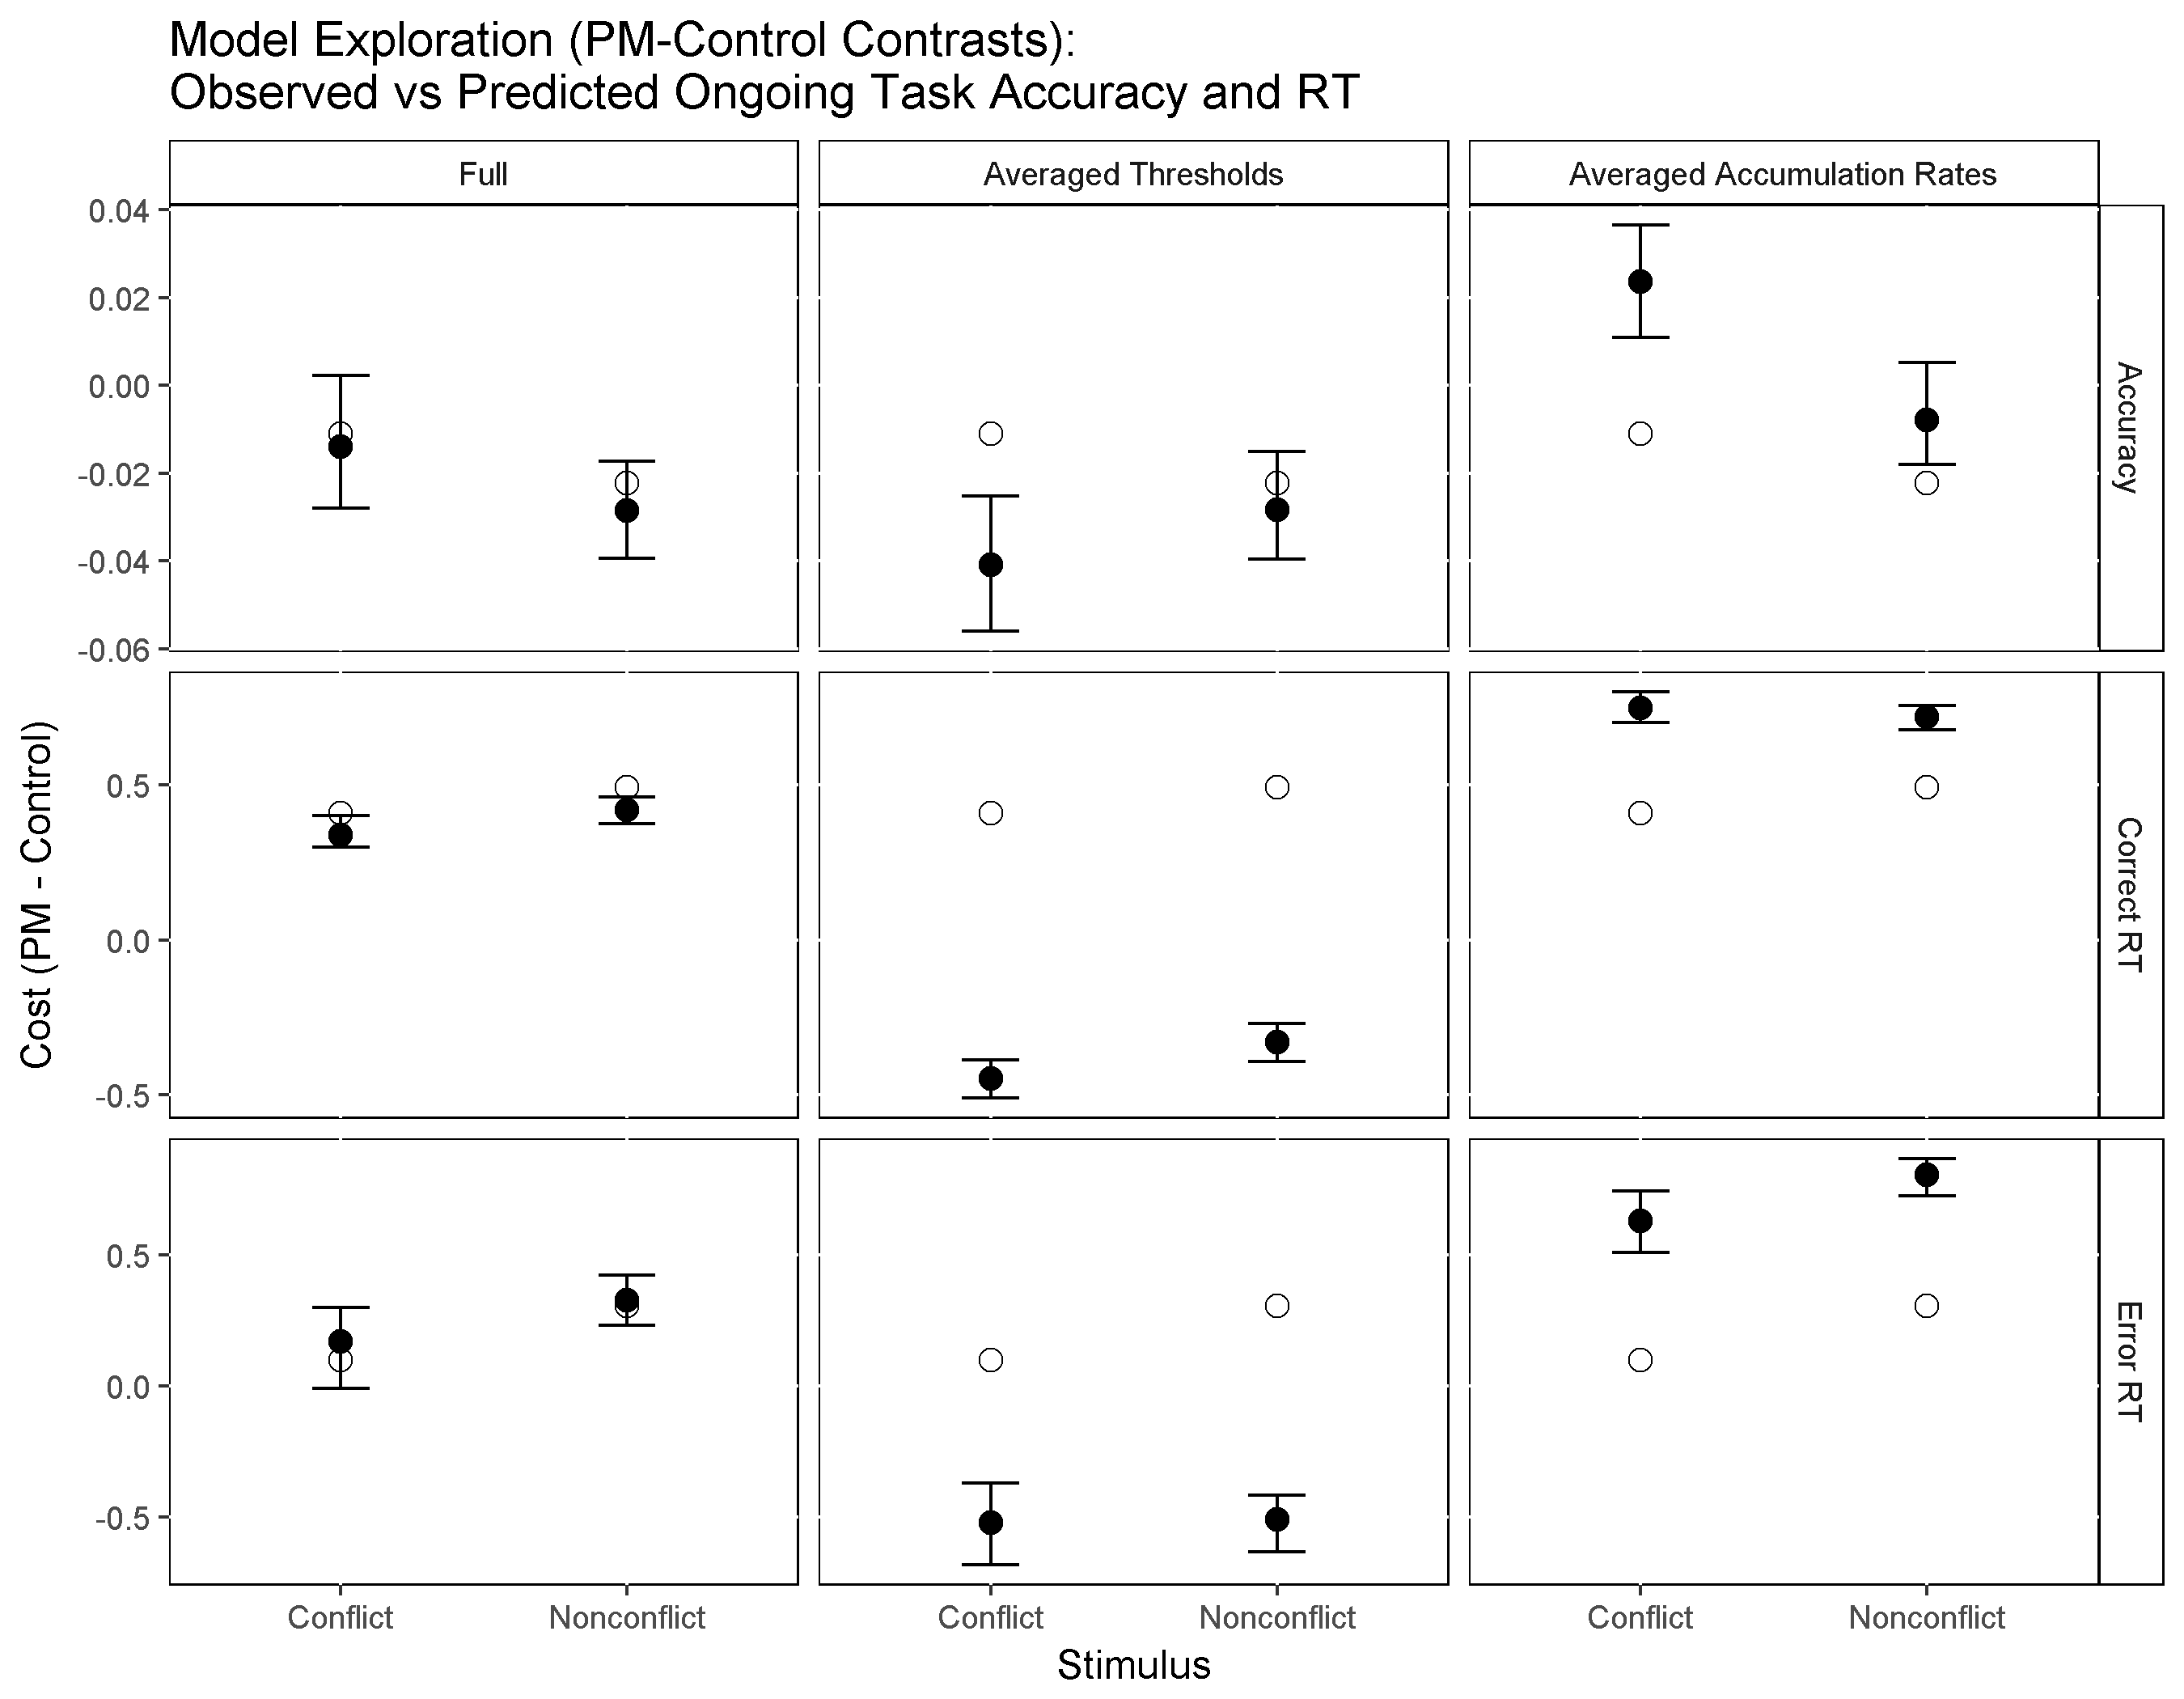
\includegraphics[width=0.5\linewidth]{figures/E1/E1.PM.Control.Contrast.Plots}
\textbackslash{}caption\{\label{fig:PM.Control.Contrast.Plots}Model
Exploration: Comparison of Accuracy and RT Fits for Models with
Thresholds or Rates Averaged over PM-Control Blocks. Data effects are
represented by white dots. Model predictions are represented by black
dots with 95\% credible
intervals.\}\label{fig:Plot: Model Exploration PM Contrasts}
\textbackslash{}end\{figure\}

\textbackslash{}begin\{figure\}
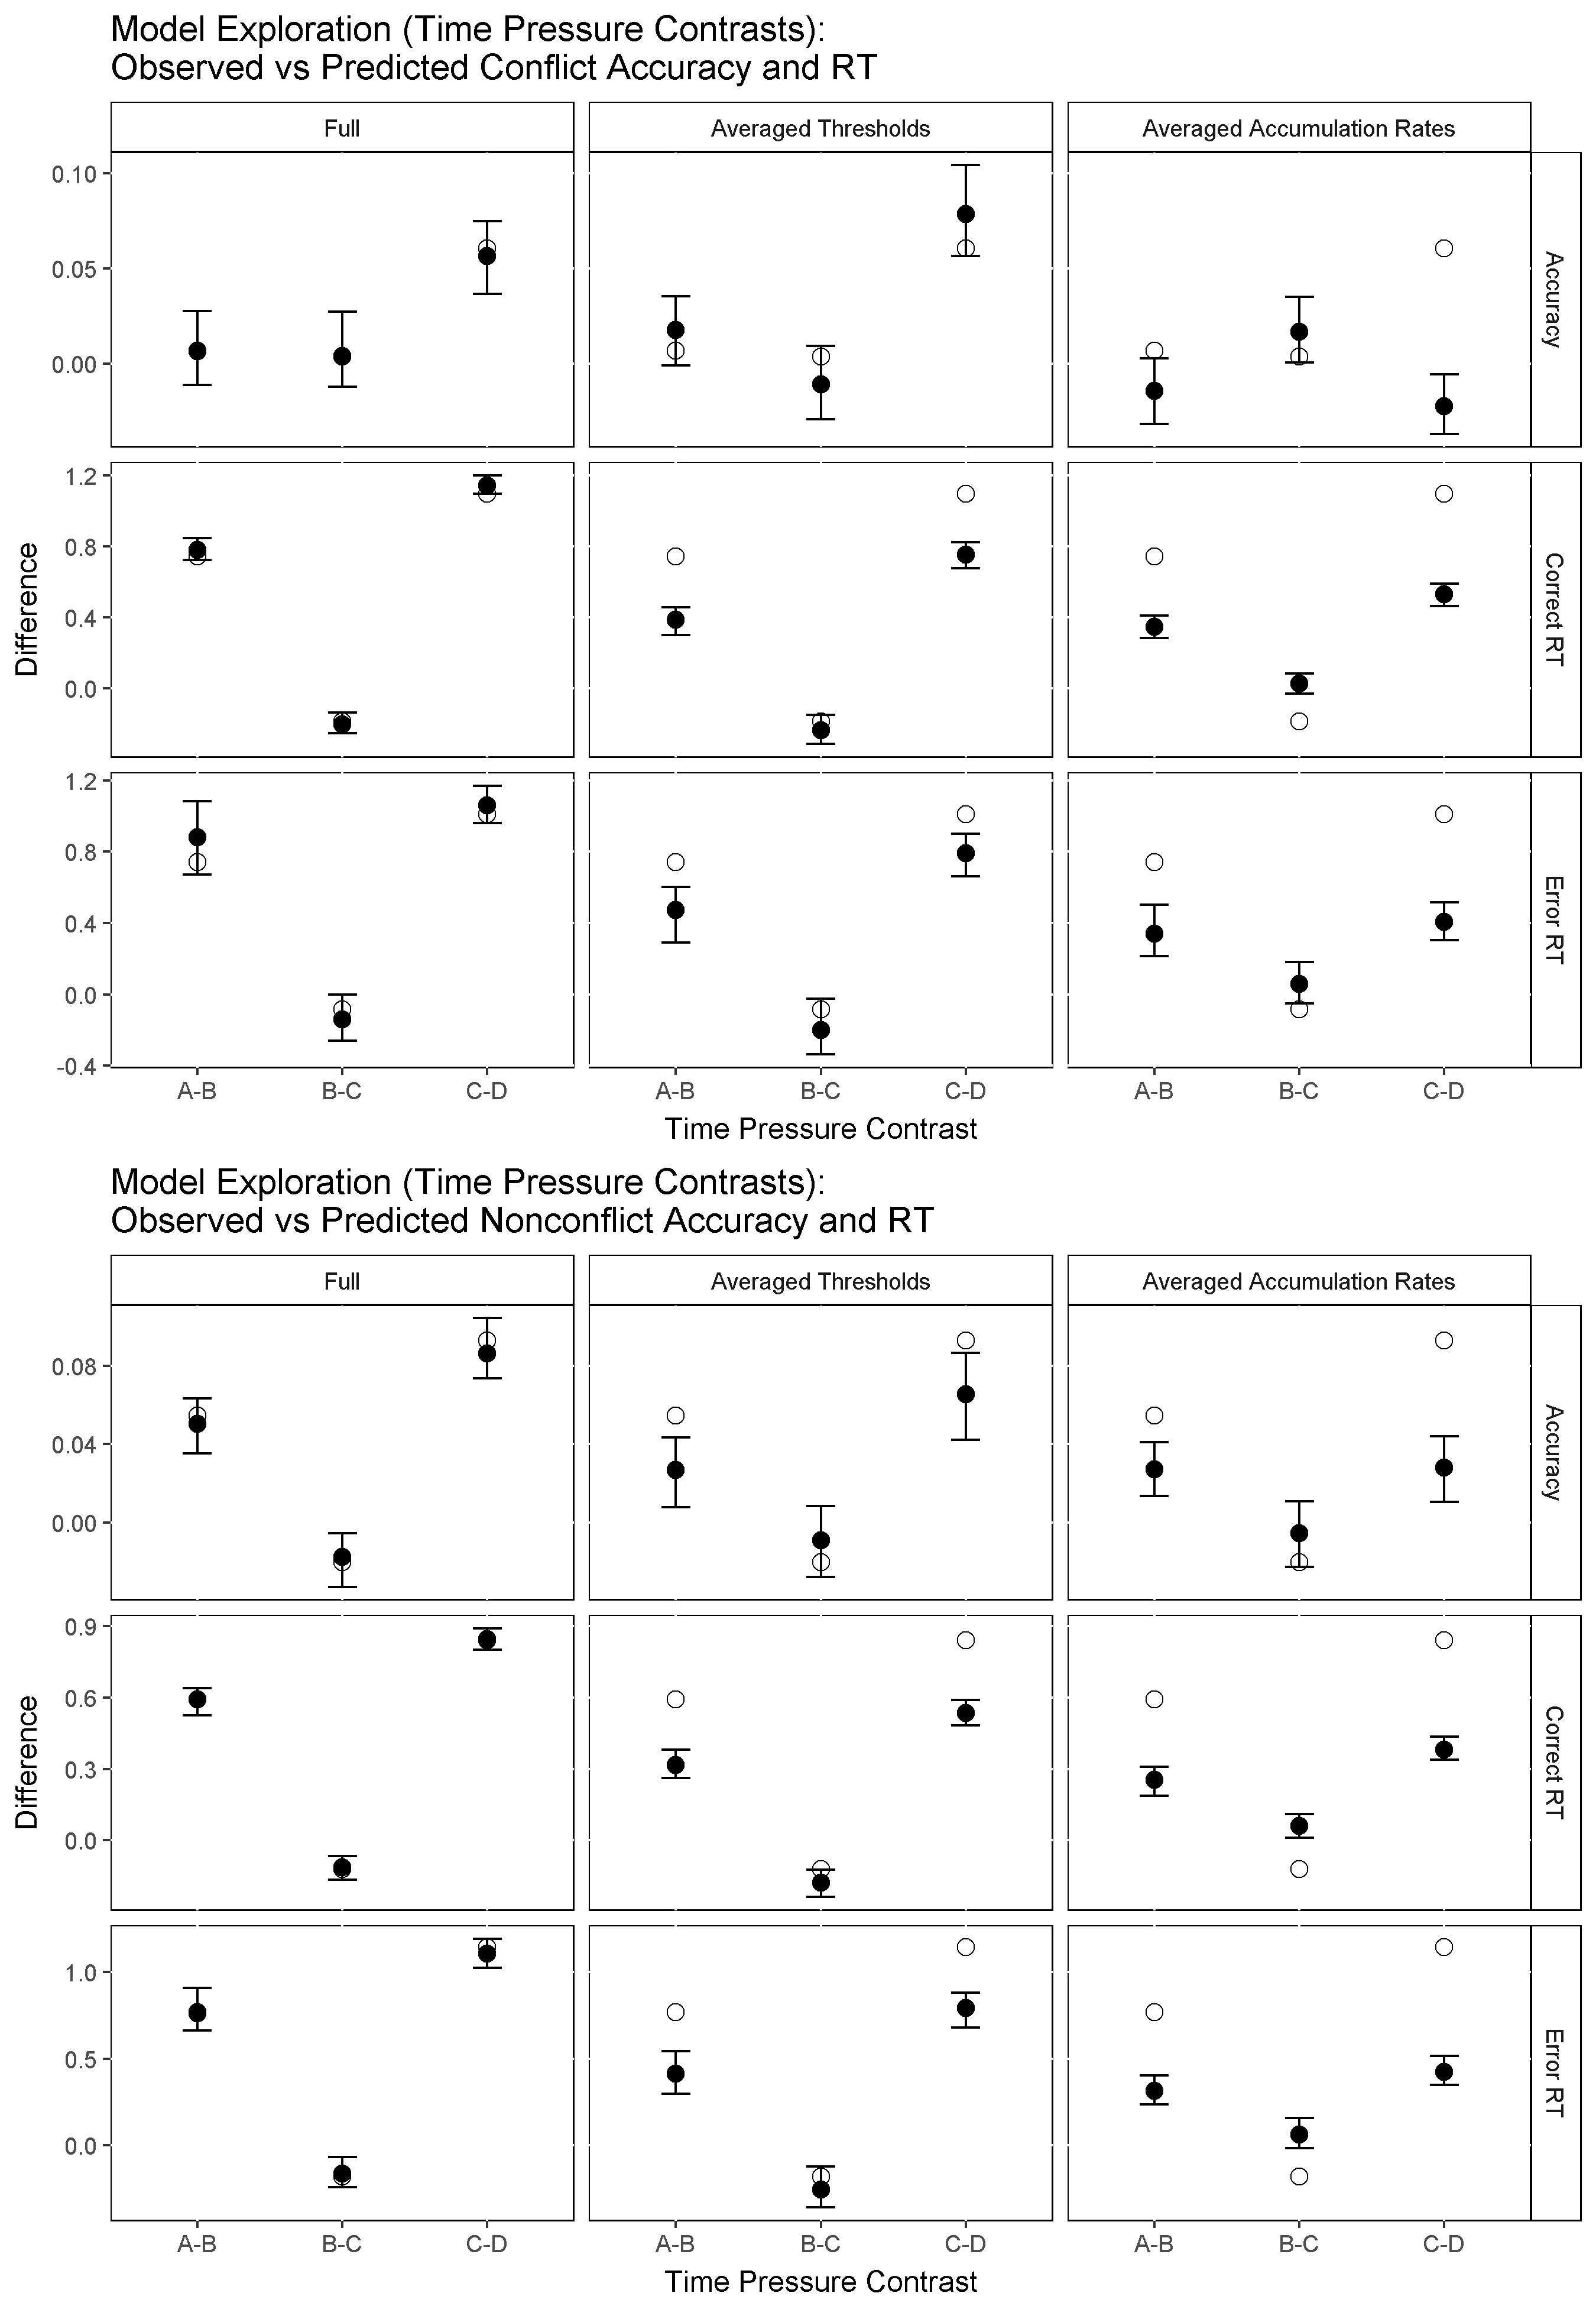
\includegraphics[width=0.5\linewidth]{figures/E1/E1.ModelExpTPContrastsOngoing}
\textbackslash{}caption\{\label{fig:ModelExpTPContrastsOngoing}Model
Exploration: Comparison of Ongoing Task Accuracy and RT Fits for Models
with Thresholds or Rates Averaged over Time Pressure Conditions. Data
effects are represented by white dots. Model predictions are represented
by black dots with 95\% credible
intervals.\}\label{fig:Plot: Model Exploration TP Contrasts}
\textbackslash{}end\{figure\}

\textbackslash{}begin\{figure\}
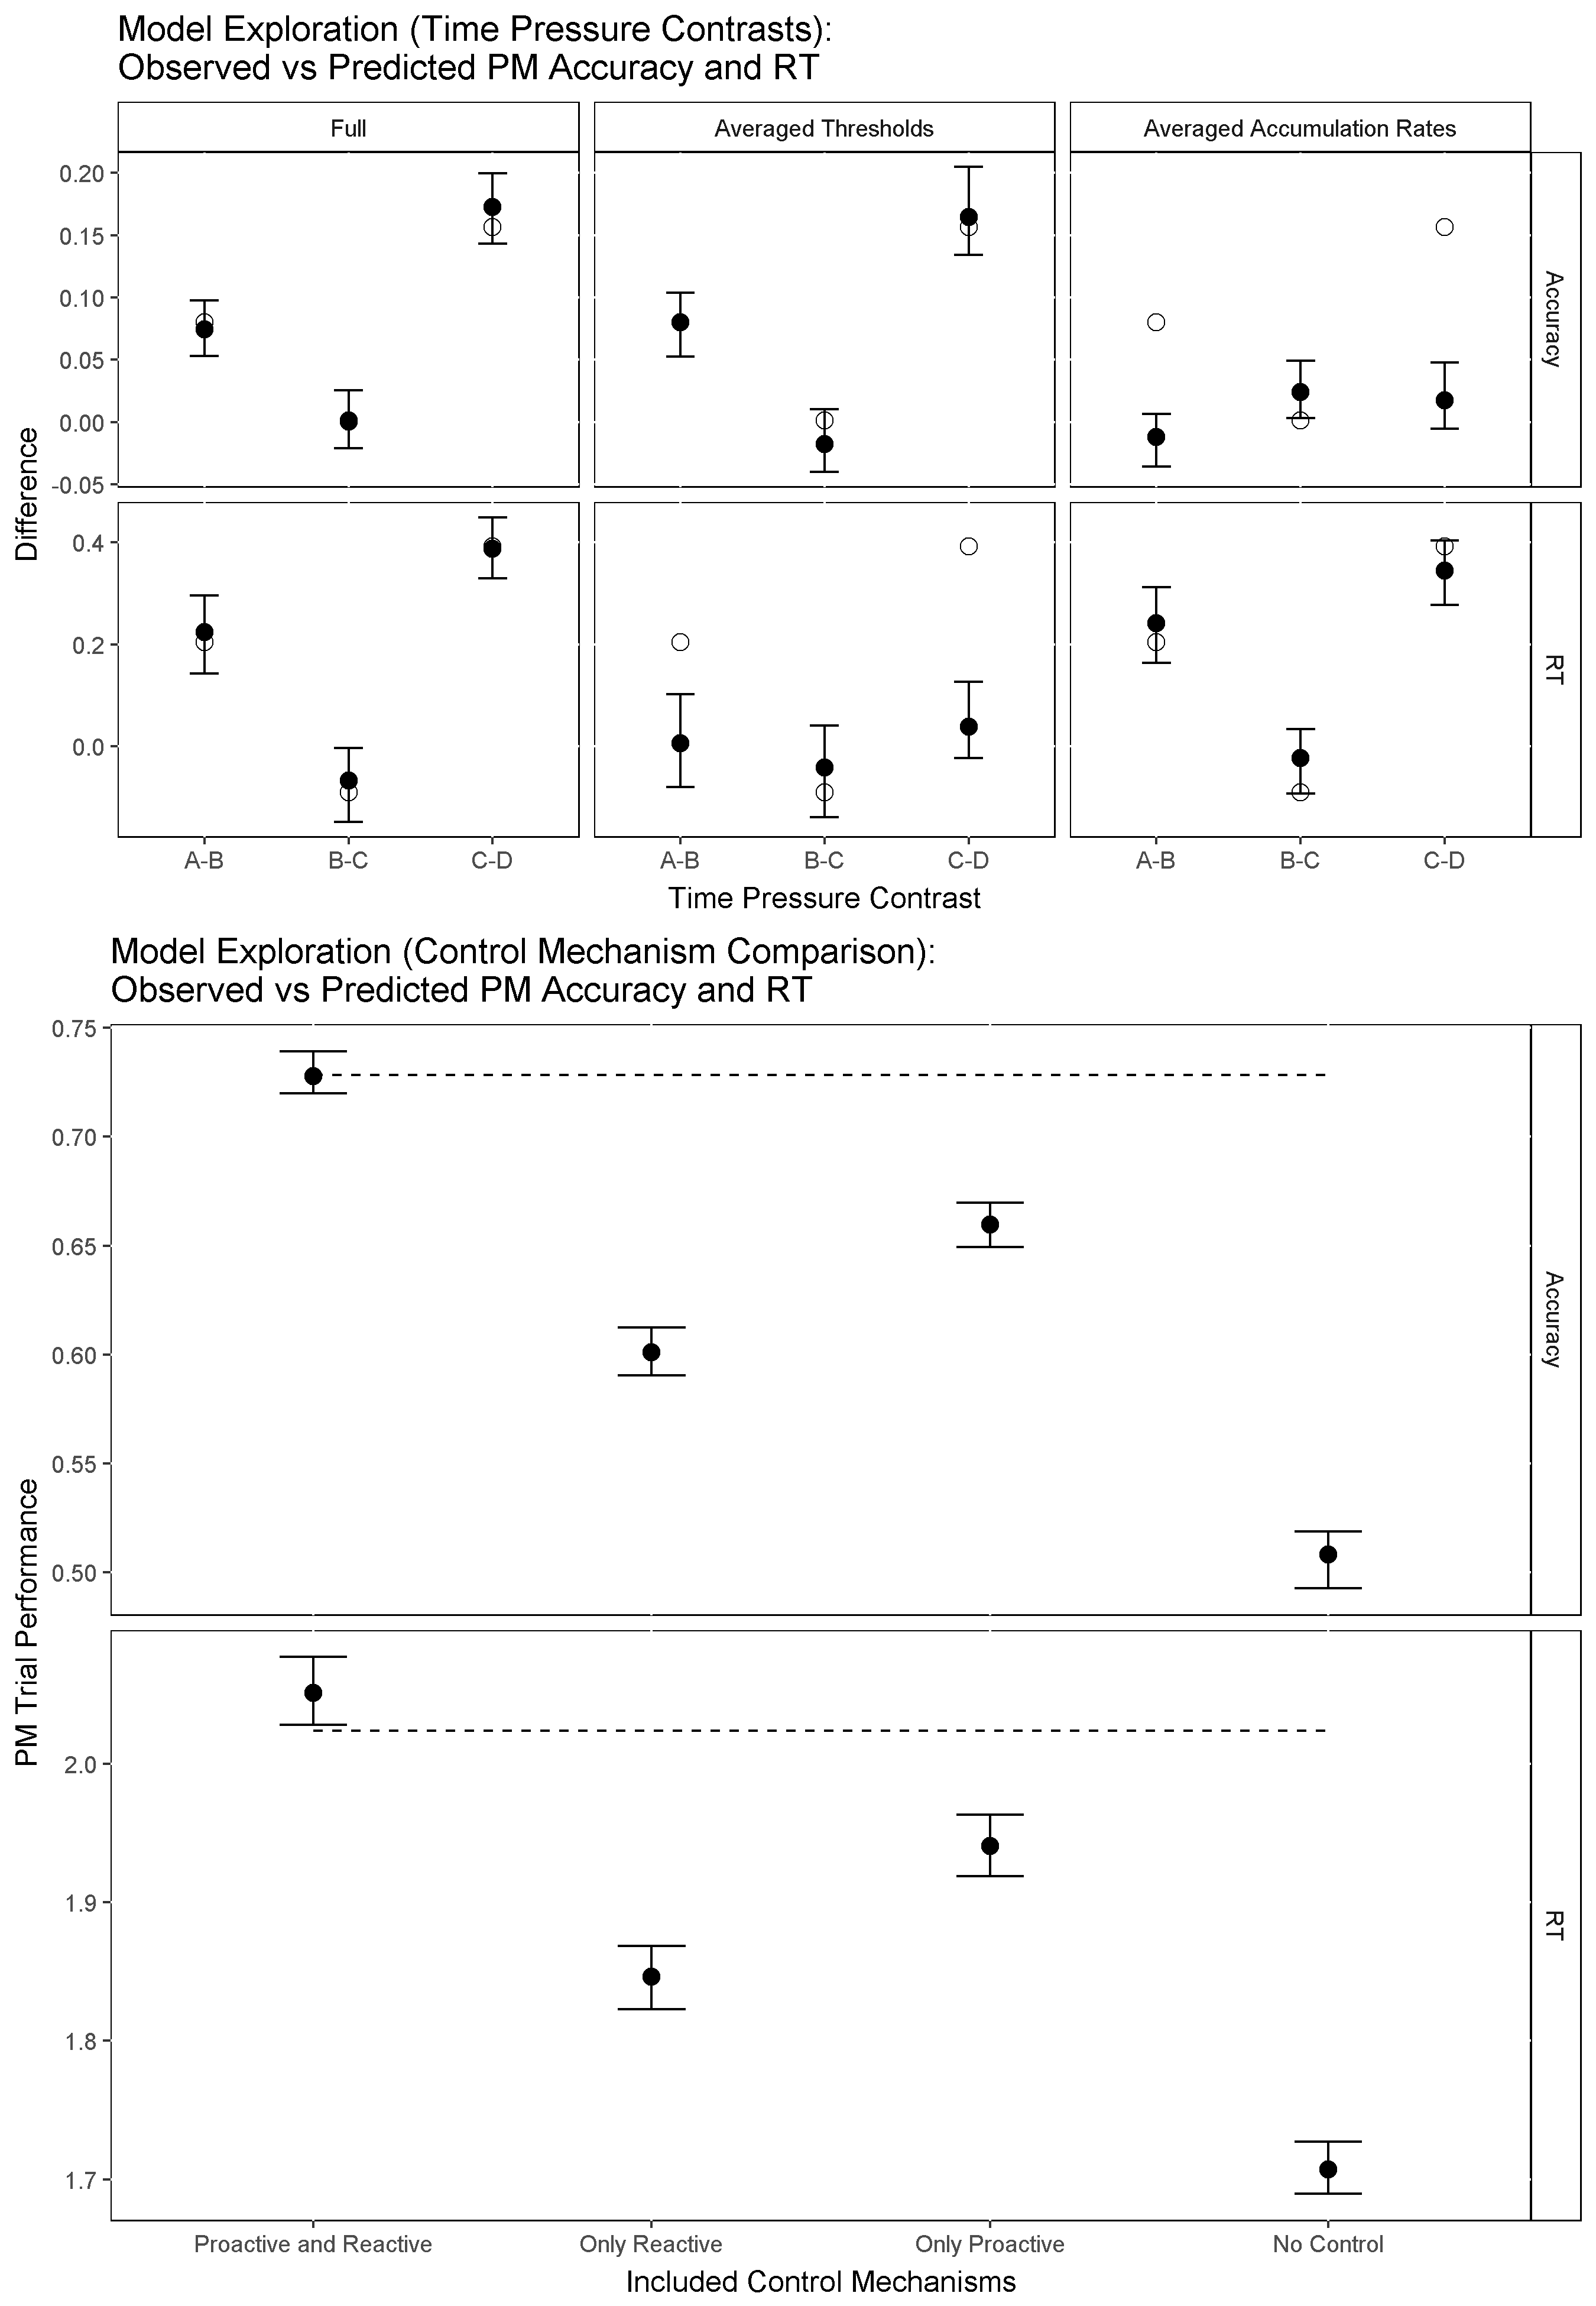
\includegraphics[width=0.5\linewidth]{figures/E1/E1.ModelExpTPContrastsPM_ControlMech}
\textbackslash{}caption\{\label{fig:ModelExpTPContrastsPM_ControlMech}Top
Panel: Model Exploration: Comparison of PM Accuracy and RT Fits for
Models with Thresholds or Rates Averaged over Time Pressure Conditions.
Bottom Panel: Model Exploration: Comparison of Accuracy and RT Fits for
Models with Cognitive Control Mechanisms Selectively Removed. Data
effects are represented by white dots. Model predictions are represented
by black dots with 95\% credible
intervals.\}\label{fig:Plot: Model Exploration TP Contrasts PM & Control Mechanisms}
\textbackslash{}end\{figure\}


\end{document}
